% !Mode:: "TeX:UTF-8"

\def\usewhat{xelatex} % 定义编译方式 pdflatex, dvipdfmx, or xelatex

\def \xuewei{Master} % 定义学位 Doctor or Master

\def\xueke{Engineering} % 定义学科 Engineering, Science, Management, Arts, Philosophy, Economics, Laws, Education, or History

\documentclass[cs4size,openany,twoside,UTF8,normalindentfirst,nofonts]{ctexbook}

% !Mode:: "TeX:UTF-8" 

\makeatletter
\@tempcnta=128
\loop \catcode\@tempcnta=13 \ifnum\@tempcnta<255 \advance \@tempcnta \@ne
\repeat
\makeatother

\newif\ifxueweidoctor %判断论文类型
\newif\ifxueweimaster
\def\temp{Doctor}
\ifx\temp\xuewei
  \xueweidoctortrue  \xueweimasterfalse
\fi
\def\temp{Master}
\ifx\temp\xuewei
  \xueweidoctorfalse  \xueweimastertrue
\fi

\ifxueweidoctor
  \newcommand{\cxuewei}{博士}
  \newcommand{\exuewei}{Doctor}
  \newcommand{\exueweier}{Doctoral}
  \newcommand{\xueweishort}{博}
\fi

\ifxueweimaster
  \newcommand{\cxuewei}{硕士}
  \newcommand{\exuewei}{Master}
  \newcommand{\exueweier}{Master's}
  \newcommand{\xueweishort}{硕}
\fi    % 硕博类型
% !Mode:: "TeX:UTF-8"
\usepackage{xeCJK}
\usepackage{tabularx}
\usepackage{graphicx}
\usepackage[a4paper,text={150true mm,224true mm},top=35.5true mm,left=30true mm,head=5true mm,headsep=2.5true mm,foot=8.5true mm]{geometry}
\usepackage{titlesec}               % 控制标题的宏包
\usepackage{titletoc}                   % 控制目录的宏包
\usepackage{fancyhdr}                   % fancyhdr宏包 页眉和页脚的相关定义
\usepackage{color}          % 支持彩色
\usepackage{amsmath}        % AMSLaTeX宏包 用来排出更加漂亮的公式
\usepackage{amssymb}
\usepackage[below]{placeins}%允许上一个section的浮动图形出现在下一个section的开始部分,还提供\FloatBarrier命令,使所有未处理的浮动图形立即被处理
\usepackage{flafter}       % 使得所有浮动体不能被放置在其浮动环境之前,以免浮动体在引述它的文本之前出现.
\usepackage{multirow}       %使用Multirow宏包,使得表格可以合并多个row格
\usepackage{booktabs}       % 表格,横的粗线;\specialrule{1pt}{0pt}{0pt}
\usepackage{longtable}      %支持跨页的表格。
\usepackage[hang]{subfigure}%支持子图 %centerlast 设置最后一行是否居中
\usepackage[subfigure]{ccaption} %支持双语标题
\usepackage[sort&compress,numbers]{natbib}% 支持引用缩写的宏包
\usepackage{enumitem}       %使用enumitem宏包,改变列表项的格式
\usepackage{calc}           %长度可以用+ - * / 进行计算
%\usepackage{txfonts}
\usepackage{fontspec}
\usepackage[amsmath,thmmarks,hyperref]{ntheorem}% 定理类环境宏包,其中 amsmath 选项用来兼容 AMS LaTeX 的宏包
\usepackage{etoolbox}
\AtBeginDocument{%
  \apptocmd\thebibliography{\interlinepenalty=1000 }{}{}% 设置参考文献的空白的阈值
}

\usepackage[xetex,
            bookmarksnumbered=true,
            bookmarksopen=true,
            colorlinks=false,
            pdfborder={0 0 1},
            citecolor=blue,
            linkcolor=red,
            anchorcolor=green,
            urlcolor=blue,
            breaklinks=true,
            naturalnames  %与algorithm2e宏包协调
            ]{hyperref}

\defaultfontfeatures{Mapping=tex-text}
\xeCJKsetemboldenfactor{1}%只对随后定义的CJK字体有效
\setCJKfamilyfont{hei}{SimHei}
\xeCJKsetemboldenfactor{4}
\setCJKfamilyfont{song}{SimSun}
\xeCJKsetemboldenfactor{1}
\setCJKfamilyfont{fs}{FangSong}
\setCJKfamilyfont{kai}{KaiTi}
\setCJKfamilyfont{li}{LiSu}
\setCJKfamilyfont{xw}{STXinwei}
\setCJKmainfont{SimSun}
\setCJKsansfont{SimHei}
\setmainfont{Times New Roman}
\setsansfont{Arial}
\newcommand{\hei}{\CJKfamily{hei}}% 黑体   (Windows自带simhei.ttf)
\newcommand{\song}{\CJKfamily{song}}    % 宋体   (Windows自带simsun.ttf)
\newcommand{\fs}{\CJKfamily{fs}}        % 仿宋体 (Windows自带simfs.ttf)
\newcommand{\kaishu}{\CJKfamily{kai}}      % 楷体   (Windows自带simkai.ttf)
\newcommand{\li}{\CJKfamily{li}}        % 隶书   (Windows自带simli.ttf)
\newcommand{\xw}{\CJKfamily{xw}}        % 隶书   (Windows自带simli.ttf)
\newfontfamily\arial{Arial}
\newfontfamily\timesnewroman{Times New Roman}

\usepackage[plainruled,linesnumbered,algochapter]{algorithm2e}  % 算法的宏包,注意宏包兼容性,先后顺序为float、hyperref、algorithm(2e),否则无法生成算法列表
\usepackage{xltxtra}
\usepackage{listings}
\lstset{
%basicstyle=\small\ttfamily,
columns=flexible,
breaklines=true
}
\newcommand{\emultiline}[2][c]{\renewcommand{\arraystretch}{1}\begin{tabular}[#1]{@{}l@{}}#2\end{tabular} \renewcommand{\arraystretch}{1.3} }
%\newcommand{\citeayu}[1]{\citeauthor{#1}~(\citeyear{#1})\citeup{#1}}

 % 引用的宏包

\graphicspath{{figures/}} %定义所有的eps文件在 figures 子目录下

\begin{document}

% !Mode:: "TeX:UTF-8" 

%\newcommand{\song}{\CJKfamily{song}}    % 宋体   (Windows自带simsun.ttf)
%\newcommand{\hei}{\CJKfamily{hei}}      % 黑体   (Windows自带simhei.ttf)
%\newcommand{\kaishu}{\CJKfamily{kai}}      % 黑体   (Windows自带simhei.ttf)

\newcommand{\yihao}{\fontsize{26pt}{26pt}\selectfont}       % 一号, 1.倍行距
\newcommand{\xiaoyi}{\fontsize{24pt}{24pt}\selectfont}      % 小一, 1.倍行距
\newcommand{\erhao}{\fontsize{22pt}{1.25\baselineskip}\selectfont}       % 二号, 1.倍行距
\newcommand{\xiaoer}{\fontsize{18pt}{18pt}\selectfont}      % 小二, 单倍行距
\newcommand{\sanhao}{\fontsize{16pt}{16pt}\selectfont}      % 三号, 1.倍行距
\newcommand{\xiaosan}{\fontsize{15pt}{15pt}\selectfont}     % 小三, 1.倍行距
\newcommand{\sihao}{\fontsize{14pt}{14pt}\selectfont}       % 四号, 1.0倍行距
\newcommand{\xiaosi}{\fontsize{12pt}{12pt}\selectfont}      % 小四, 1.倍行距
\newcommand{\wuhao}{\fontsize{10.5pt}{10.5pt}\selectfont}   % 五号, 单倍行距
\newcommand{\xiaowu}{\fontsize{9pt}{9pt}\selectfont}        % 小五, 单倍行距


%避免宏包 hyperref 和 arydshln 不兼容带来的目录链接失效的问题。
\def\temp{\relax}
\let\temp\addcontentsline
\gdef\addcontentsline{\phantomsection\temp}

\makeatletter
\gdef\hitempty{}

%重新定义BiChapter命令,可实现标题手动换行,但不影响目录
\def\BiChapter{\relax\@ifnextchar [{\@BiChapter}{\@@BiChapter}}
\def\@BiChapter[#1]#2#3{\chapter[#1]{#2}
    \addcontentsline{toe}{chapter}{\bfseries \xiaosi Chapter \thechapter\hspace{0.5em} #3}}
\def\@@BiChapter#1#2{\chapter{#1}
    \addcontentsline{toe}{chapter}{\bfseries \xiaosi Chapter \thechapter\hspace{0.5em}{\boldmath #2}}}

\newcommand{\BiSection}[2]
{   \section{#1}
    \addcontentsline{toe}{section}{\protect\numberline{\csname thesection\endcsname}#2}
}

\newcommand{\BiSubsection}[2]
{    \subsection{#1}
    \addcontentsline{toe}{subsection}{\protect\numberline{\csname thesubsection\endcsname}#2}
}

\newcommand{\BiSubsubsection}[2]
{    \subsubsection{#1}
    \addcontentsline{toe}{subsubsection}{\protect\numberline{\csname thesubsubsection\endcsname}#2}
}

\newcommand{\BiAppendixChapter}[2] % 该附录命令适用于发表文章,简历等
{\phantomsection
\markboth{#1}{#1}
\addcontentsline{toc}{chapter}{\xiaosi #1}
\addcontentsline{toe}{chapter}{\bfseries \xiaosi #2}  \chapter*{#1}
}

\newcommand{\BiAppChapter}[2]    % 该附录命令适用于有章节的完整附录
{\phantomsection 
 \chapter{#1}
 \addcontentsline{toe}{chapter}{\bfseries \xiaosi Appendix \thechapter~~#2}
}

\renewcommand{\thefigure}{\arabic{chapter}-\arabic{figure}}%使图编号为 7-1 的格式 %\protect{~}
\renewcommand{\thesubfigure}{\alph{subfigure})}%使子图编号为 a)的格式
\renewcommand{\p@subfigure}{\thefigure~} %使子图引用为 7-1 a) 的格式,母图编号和子图编号之间用~加一个空格
\renewcommand{\thetable}{\arabic{chapter}-\arabic{table}}%使表编号为 7-1 的格式
\renewcommand{\theequation}{\arabic{chapter}-\arabic{equation}}%使公式编号为 7-1 的格式

\newcommand{\algoenname}{Algo.} %算法英文标题
\newfloatlist[chapter]{algoen}{aen}{\listalgoenname}{\algoenname}
\newfixedcaption{\algoencaption}{algoen}
\renewcommand{\thealgoen}{\thechapter-\arabic{algocf}}
\renewcommand{\@cftmakeaentitle}{\chapter*{\listalgoenname\@mkboth{\bfseries\listalgoenname}{\bfseries\listalgoenname}}}

\renewcommand{\algorithmcfname}{算法}
\setlength\AlCapSkip{1.2ex}
\SetAlgoSkip{1pt}
\renewcommand{\algocf@captiontext}[2]{\wuhao#1\algocf@typo ~ \AlCapFnt{}#2} % text of caption
\expandafter\ifx\csname algocf@within\endcsname\relax% if \algocf@within doesn't exist
\renewcommand\thealgocf{\@arabic\c@algocf} % and the way it is printed
\else%                                    else
\renewcommand\thealgocf{\csname the\algocf@within\endcsname-\@arabic\c@algocf}
\fi
\renewcommand{\algocf@makecaption}[2]{%中英文双标题一定多于一行,因此去掉单行时的判断,并将\parbox中标题设置为居中
  \addtolength{\hsize}{\algomargin}%
  \sbox\@tempboxa{\algocf@captiontext{#1}{#2}}%
    \hskip .5\algomargin%
    \parbox[t]{\hsize}{\centering\algocf@captiontext{#1}{#2}}% 
  \addtolength{\hsize}{-\algomargin}%
}
\newcommand{\AlgoBiCaption}[2]{%直接取出自定义的中英文标题条目加入到真正的\caption 中  
   \caption[#1]{\protect\setlength{\baselineskip}{1.5em}#1 \protect \\ Algo. \thealgocf~~ #2} % \algoencaption{#2}   
   \addcontentsline{aen}{algoen}{\protect\numberline{\thealgoen}{#2}}
   }

\setlength{\algoheightruledefault}{1.5pt}
\newcommand{\foocaption}[1]{ \def\@algocf@pre@plainruled{\hrule height1.5pt depth0pt\kern\interspacetitleruled #1 \kern\interspacealgoruled\hrule height1pt depth0pt\kern\interspacetitleruled} }
\def\@algocf@post@ruled{\kern\interspacealgoruled\hrule height1.5pt\relax}%
\makeatother

%定义 学科 学位
\def \xuekeEngineering {Engineering}
\def \xuekeScience {Science}
\def \xuekeManagement {Management}
\def \xuekeArts {Arts}
\def \xuekePhilosophy {Philosophy}
\def \xuekeEconomics {Economics}
\def \xuekeLaws {Laws}
\def \xuekeEducation {Education}
\def \xuekeHistory {History}


\ifx \xueke \xuekeEngineering
\newcommand{\cxueke}{工学}
\newcommand{\exueke}{Engineering}
\fi

\ifx \xueke \xuekeScience
\newcommand{\cxueke}{理学}
\newcommand{\exueke}{Science}
\fi

\ifx \xueke \xuekeManagement
\newcommand{\cxueke}{管理学}
\newcommand{\exueke}{Management}
\fi

\ifx \xueke \xuekeArts
\newcommand{\cxueke}{文学}
\newcommand{\exueke}{Arts}
\fi 

\ifx \xueke \xuekePhilosophy
\newcommand{\cxueke}{哲学}
\newcommand{\exueke}{Philosophy}
\fi 

\ifx \xueke \xuekeEconomics
\newcommand{\cxueke}{经济学}
\newcommand{\exueke}{Economics}
\fi 

\ifx \xueke \xuekeLaws
\newcommand{\cxueke}{法学}
\newcommand{\exueke}{Laws}
\fi 

\ifx \xueke \xuekeEducation
\newcommand{\cxueke}{教育学}
\newcommand{\exueke}{Education}
\fi 

\ifx \xueke \xuekeHistory
\newcommand{\cxueke}{历史学}
\newcommand{\exueke}{History}
\fi 
 % 文本格式定义
% !Mode:: "TeX:UTF-8" 

\theoremstyle{plain}
\theorembodyfont{\song\rmfamily}
\theoremheaderfont{\hei\rmfamily}
\newtheorem{definition}{\hei 定义}[chapter]
\newtheorem{example}{\hei 例}[chapter]
\newtheorem{algo}{\hei 算法}[chapter]
\newtheorem{theorem}{\hei 定理}[chapter]
\newtheorem{axiom}{\hei 公理}[chapter]
\newtheorem{proposition}{\hei 命题}[chapter]
\newtheorem{lemma}{\hei 引理}[chapter]
\newtheorem{corollary}{\hei 推论}[chapter]
\newtheorem{remark}{\hei 注解}[chapter]
\newenvironment{proof}{\noindent{\hei 证明:}}{\hfill $ \square $ \vskip 4mm}
\theoremsymbol{$\square$}
\setlength{\theorempreskipamount}{0pt}
\setlength{\theorempostskipamount}{-2pt}

\allowdisplaybreaks[4]

%\CJKcaption {gb_452} 
%\CJKtilde
\setlength{\parindent}{2em}

\arraycolsep=1.6pt

\renewcommand\contentsname{\hei 目~~~~录}

\CTEXsetup[number={\arabic{chapter}}]{chapter}
\renewcommand\chaptername{第~\thechapter~章}

%\CTEXsetup[name={第,章}]{chapter}
\setcounter{secnumdepth}{4} \setcounter{tocdepth}{2}


\titleformat{\chapter}{\center\xiaoer\hei}{\chaptertitlename}{0.5em}{}
\titlespacing{\chapter}{0pt}{-5.5mm}{8mm}
\titleformat{\section}{\xiaosan\hei}{\thesection}{0.5em}{}
\titlespacing{\section}{0pt}{4.5mm}{4.5mm}
\titleformat{\subsection}{\sihao\hei}{\thesubsection}{0.5em}{}
\titlespacing{\subsection}{0pt}{4mm}{4mm}
\titleformat{\subsubsection}{\xiaosi\hei}{\thesubsubsection}{0.5em}{}
\titlespacing{\subsubsection}{0pt}{0pt}{0pt}

\titlecontents{chapter}[3.8em]{\hspace{-3.8em}\hei}{\thecontentslabel~~}{}{\titlerule*[4pt]{.}\contentspage}
\dottedcontents{section}[32pt]{}{21pt}{0.3pc}
\dottedcontents{subsection}[53pt]{}{30pt}{0.3pc}


% 按工大标准, 缩小目录中各级标题之间的缩进,使它们相隔一个字符距离,也就是12pt
\makeatletter
\renewcommand*\l@chapter{\@dottedtocline{0}{0em}{5em}}%控制英文目录: 细点\@dottedtocline  粗点\@dottedtoclinebold
\renewcommand*\l@section{\@dottedtocline{1}{1em}{1.8em}}
\renewcommand*\l@subsection{\@dottedtocline{2}{2em}{2.5em}}


% 定义页眉和页脚
\newcommand{\makeheadrule}{
\rule[7pt]{\textwidth}{0.75pt} \\[-23pt]
\rule{\textwidth}{2.25pt}}
\renewcommand{\headrule}{
    {\if@fancyplain\let\headrulewidth\plainheadrulewidth\fi
     \makeheadrule}}
\pagestyle{fancyplain}

%去掉章节标题中的数字
%%不要注销这一行,否则页眉会变成:“第1章1  绪论”样式
\renewcommand{\chaptermark}[1]{\markboth{\chaptertitlename~\ #1}{}}
\fancyhf{}

%在book文件类别下,\leftmark自动存录各章之章名,\rightmark记录节标题
%% 页眉字号 工大要求 小五
%根据单双面打印设置不同的页眉;

\ifxueweidoctor
  \fancyhead[CO]{\song \xiaowu\leftmark}
  \fancyhead[CE]{\song \xiaowu 哈尔滨工业大学\cxueke\cxuewei 学位论文}%
  \fancyfoot[C,C]{\xiaowu -~\thepage~-}
\else
  \fancyhead[CO]{\song \xiaowu 哈尔滨工业大学\cxueke\cxuewei 学位论文}
  \fancyhead[CE]{\song \xiaowu 哈尔滨工业大学\cxueke\cxuewei 学位论文}%
  \fancyfoot[C,C]{\xiaowu -~\thepage~-}
\fi

\renewcommand\frontmatter{\cleardoublepage
  \@mainmatterfalse
  \pagenumbering{Roman}}

% 调整罗列环境的布局
\setitemize{leftmargin=0em,itemsep=0em,partopsep=0em,parsep=0em,topsep=0em,itemindent=3em}
\setenumerate{leftmargin=0em,itemsep=0em,partopsep=0em,parsep=0em,topsep=0em,itemindent=3.5em}

\newcommand{\citeup}[1]{\textsuperscript{\cite{#1}}}

% 定制浮动图形和表格标题样式
\captionnamefont{\wuhao}
\captiontitlefont{\wuhao}
\captiondelim{~~}
%\captionstyle{\hang}
\hangcaption
\renewcommand{\subcapsize}{\wuhao}
\setlength{\abovecaptionskip}{0pt}
\setlength{\belowcaptionskip}{0pt}

% 自定义项目列表标签及格式 \begin{publist} 列表项 \end{publist}
\newcounter{pubctr} %自定义新计数器
\newenvironment{publist}{%%%%%定义新环境
\begin{list}{[\arabic{pubctr}]} %%标签格式
    {
     \usecounter{pubctr}
     \setlength{\leftmargin}{1.7em}     % 左边界 \leftmargin =\itemindent + \labelwidth + \labelsep
     \setlength{\itemindent}{0em}     % 标号缩进量
     \setlength{\labelsep}{0.5em}       % 标号和列表项之间的距离,默认0.5em
     \setlength{\rightmargin}{0em}    % 右边界
     \setlength{\topsep}{0ex}         % 列表到上下文的垂直距离
     \setlength{\parsep}{0ex}         % 段落间距
     \setlength{\itemsep}{0ex}        % 标签间距
     \setlength{\listparindent}{0pt} % 段落缩进量
    }}
{\end{list}}%%%%%

% 默认字体
\renewcommand\normalsize{
  \@setfontsize\normalsize{12pt}{12pt}
  \setlength\abovedisplayskip{4pt}
  \setlength\abovedisplayshortskip{4pt}
  \setlength\belowdisplayskip{\abovedisplayskip}
  \setlength\belowdisplayshortskip{\abovedisplayshortskip}
  \let\@listi\@listI}
  
% 设置行距和段落间垂直距离
\def\defaultfont{\renewcommand{\baselinestretch}{1.62}\normalsize\selectfont}
\renewcommand{\CJKglue}{\hskip 0.56pt plus 0.08\baselineskip} 
%加大字间距,使每行34个字,若要使得每行33个字,则将0.56pt替换为0.96pt。
\predisplaypenalty=0  %公式之前可以换页,公式出现在页面顶部

% 封面、摘要、版权、致谢格式定义
\def\ctitle#1{\def\@ctitle{#1}}\def\@ctitle{}
\def\cdegree#1{\def\@cdegree{#1}}\def\@cdegree{}
\def\caffil#1{\def\@caffil{#1}}\def\@caffil{}
\def\csubject#1{\def\@csubject{#1}}\def\@csubject{}
\def\cauthor#1{\def\@cauthor{#1}}\def\@cauthor{}
\def\csupervisor#1{\def\@csupervisor{#1}}\def\@csupervisor{}
\def\cassosupervisor#1{\def\@cassosupervisor{{\hei 副 \hfill 导 \hfill 师} & #1\\}}\def\@cassosupervisor{}
\def\ccosupervisor#1{\def\@ccosupervisor{{\hei 联 \hfill 合\hfill 导 \hfill 师} & #1\\}}\def\@ccosupervisor{}
\def\cdate#1{\def\@cdate{#1}}\def\@cdate{}
\long\def\cabstract#1{\long\def\@cabstract{#1}}\long\def\@cabstract{}
\def\ckeywords#1{\def\@ckeywords{#1}}\def\@ckeywords{}

\def\etitle#1{\def\@etitle{#1}}\def\@etitle{}
\def\edegree#1{\def\@edegree{#1}}\def\@edegree{}
\def\eaffil#1{\def\@eaffil{#1}}\def\@eaffil{}
\def\esubject#1{\def\@esubject{#1}}\def\@esubject{}
\def\eauthor#1{\def\@eauthor{#1}}\def\@eauthor{}
\def\esupervisor#1{\def\@esupervisor{#1}}\def\@esupervisor{}
\def\eassosupervisor#1{\def\@eassosupervisor{\textbf{Associate Supervisor:} & #1\\}}\def\@eassosupervisor{}
\def\ecosupervisor#1{\def\@ecosupervisor{\textbf{Co Supervisor:} & #1\\}}\def\@ecosupervisor{}
\def\edate#1{\def\@edate{#1}}\def\@edate{}
\long\def\eabstract#1{\long\def\@eabstract{#1}}\long\def\@eabstract{}
\long\def\NotationList#1{\long\def\@NotationList{#1}}\long\def\@NotationList{}
\def\ekeywords#1{\def\@ekeywords{#1}}\def\@ekeywords{}
\def\natclassifiedindex#1{\def\@natclassifiedindex{#1}}\def\@natclassifiedindex{}
\def\internatclassifiedindex#1{\def\@internatclassifiedindex{#1}}\def\@internatclassifiedindex{}
\def\statesecrets#1{\def\@statesecrets{#1}}\def\@statesecrets{}

% 定义封面
\def\makecover{
    \begin{titlepage}
    % 封面一
   \vspace*{0.8cm}
   \begin{center}
    \centerline{\xiaoyi\textbf\song{\cxuewei 学位论文}}

    \vspace{1cm}

    \parbox[t][2.8cm][t]{\textwidth}{
    \begin{center}\erhao\hei\@ctitle\end{center} }

    \parbox[t][5.1cm][t]{\textwidth}{ %英文标题太长时可以采用\xiaoer
    \begin{center}\erhao\textbf{\@etitle}\end{center} }

    \parbox[t][7.4cm][t]{\textwidth}{
    \begin{center}\xiaoer\textbf\song{\@cauthor}\end{center}}

    \parbox[t][1.4cm][t]{\textwidth}{
    \begin{center}\kaishu\xiaoer\textbf{哈尔滨工业大学}\end{center} }
    
    {\textbf\song\xiaoer{\@cdate}}

    \end{center}

    % 封二 空白页
    \ifxueweidoctor
      \newpage
      ~~~\vspace{1em}
      \thispagestyle{empty}
    \fi

    %内封
    \newpage
    \thispagestyle{empty}
    \pdfbookmark[0]{\@ctitle}{ctitlepage}

\begin{center}

			{\song \xiaosi
			\begin{tabular}{@{}r@{:}l@{}}
			国内图书分类号 & \@natclassifiedindex\\
 			国际图书分类号 & \@internatclassifiedindex
			\end{tabular}}\hfill
			{\song \xiaosi
			\begin{tabular}{@{}r@{:}l@{}}
			学校代码 & 10213\\
 			密级 &  公开
			\end{tabular}}
    \parbox[t][3.2cm][t]{\textwidth}{\begin{center} \end{center} }

    \parbox[t][2.4cm][t]{\textwidth}{\xiaoer
    \begin{center} {\textbf\song\@cdegree 学位论文 }\end{center} }

    \parbox[t][5cm][t]{\textwidth}{\erhao
    \begin{center} {\hei  \@ctitle}\end{center} }
	\parbox[t][9.8cm][b]{\textwidth}
     {\sihao
    \begin{center} \renewcommand{\arraystretch}{1.62} \song
    \begin{tabular}{l@{:}l}
    {\hei \xueweishort \hfill 士\hfill 研\hfill 究\hfill 生}           & \@cauthor\\
    {\hei 导\hfill 师}                       & \@csupervisor\\
	\@cassosupervisor
	\@ccosupervisor
    {\hei 申\hfill 请\hfill 学\hfill 位} & \@cdegree\\
    {\hei 学\hfill 科}           & \@csubject\\
    {\hei 所\hfill 在\hfill 单\hfill 位} & \@caffil\\
    {\hei 答\hfill 辩\hfill 日\hfill 期} & \@cdate\\
    {\hei 授予学位单位}                     & 哈尔滨工业大学
    \end{tabular} \renewcommand{\arraystretch}{1}
    \end{center} }
\end{center}

%%%%%%增加一空白页
  \ifxueweidoctor
    \newpage
    ~~~\vspace{1em}
    \thispagestyle{empty}
  \fi

    % 英文封面
    \newpage
    \thispagestyle{empty}
    \pdfbookmark[0]{\uppercase{\@etitle}}{etitlepage}

    {
    \xiaosi\noindent Classified Index: \@natclassifiedindex \\
                  U.D.C:  \@internatclassifiedindex }
    \begin{center}
    \parbox[t][1.6cm][t]{\textwidth}{\begin{center} \end{center} }
    \parbox[t][3.5cm][t]{\textwidth}{\xiaoer
    \begin{center} {  Dissertation for the {\exueweier} Degree in \exueke}\end{center} } %与中文保持一致,删除in {\exueke}

    \parbox[t][7cm][t]{\textwidth}{\erhao
    \begin{center} { \bfseries \@etitle}\end{center} }

%★★★★若信息内容不太长,不会引起信息内容分行时,使用tabular环境,否则使用下面的tabularx环境。
    {\sihao\renewcommand{\arraystretch}{1.3}
    \begin{tabular}{@{}l@{~}l@{}}
    \textbf{Candidate:}                     &  \@eauthor\\
    \textbf{Supervisor:}                    &  \@esupervisor\\
	  \@eassosupervisor
	  \@ecosupervisor
    \textbf{Academic Degree Applied for:}   &  \@edegree\\
    \textbf{Specialty:}                     &  \@esubject\\
    \textbf{Affiliation:}                   &  \@eaffil\\
    \textbf{Date of Defence:}               &  \@edate\\
    \textbf{Degree-Conferring-Institution:} &  Harbin Institute of Technology
    \end{tabular}\renewcommand{\arraystretch}{1}}

    %{\sihao\renewcommand{\arraystretch}{1.3}
    %\begin{tabularx}{\textwidth}{@{}l@{~}X@{}}
    %\textbf{Candidate:}                     &  \@eauthor\\
    %\textbf{Supervisor:}                    &  \@esupervisor\\
		%\@eassosupervisor
	  %\@ecosupervisor
    %\textbf{Academic Degree Applied for:}   &  \@edegree\\
    %\textbf{Specialty:}                     &  \@esubject\\
    %\textbf{Affiliation:}                   &  \@eaffil\\
    %\textbf{Date of Defence:}               &  \@edate\\
    %\textbf{Degree-Conferring-Institution:} &  Harbin Institute of Technology
    %\end{tabularx}\renewcommand{\arraystretch}{1}}

    \end{center}
    \end{titlepage}

%%%%%%增加一空白页
  \ifxueweidoctor
    \newpage
    ~~~\vspace{1em}
    \thispagestyle{empty}
  \fi
%%%%%%%%%%%%%%%%%%%   Abstract and keywords  %%%%%%%%%%%%%%%%%%%%%%%
\clearpage

\BiAppendixChapter{摘\quad 要}{Abstract (In Chinese)}

\setcounter{page}{1}
\song\defaultfont
\@cabstract
\vspace{\baselineskip}

\hangafter=1\hangindent=51pt\noindent
{\hei 关键词}:\@ckeywords

%%%%%%%%%%%%%%%%%%%   English Abstract  %%%%%%%%%%%%%%%%%%%%%%%%%%%%%%
\clearpage

\phantomsection
\markboth{Abstract}{Abstract}
\addcontentsline{toc}{chapter}{\xiaosi ABSTRACT}
\addcontentsline{toe}{chapter}{\bfseries \xiaosi Abstract (In English)}  
\addtocontents{toc}{\vspace{\baselineskip}}
\addtocontents{toe}{\vspace{\baselineskip}}
\chapter*{\bf Abstract}
\@eabstract
\vspace{\baselineskip}

\hangafter=1\hangindent=60pt\noindent
{\textbf{Keywords:}}  \@ekeywords
}

%%%%%%%%%%%%%%%%%%%%%%%%%%%%%%%%%%%%%%%%%%%%%%%%%%%%%%%%%%%%%%%
% 英文目录格式
\def\@dotsep{0.75}           % 定义英文目录的点间距
\setlength\leftmargini {0pt}
\setlength\leftmarginii {0pt}
\setlength\leftmarginiii {0pt}
\setlength\leftmarginiv {0pt}
\setlength\leftmarginv {0pt}
\setlength\leftmarginvi {0pt}

\def\engcontentsname{\bfseries Contents}
\newcommand\tableofengcontents{
   \pdfbookmark[0]{Contents}{econtent}
     \@restonecolfalse
   \chapter*{\engcontentsname  %chapter*上移一行,避免在toc中出现。
       \@mkboth{%
          \engcontentsname}{\engcontentsname}}
   \@starttoc{toe}%
   \if@restonecol\twocolumn\fi
   }

\urlstyle{same}  %论文中引用的网址的字体默认与正文中字体不一致,这里修正为一致的。

\renewcommand\endtable{\vspace{-4mm}\end@float}

\makeatother


\frontmatter
% !Mode:: "TeX:UTF-8" 

\newcommand{\chinesethesistitle}{局部多孔质气体静压轴承关键技术的研究} %授权书用,无需断行
\newcommand{\englishthesistitle}{\uppercase{RESEARCH ON KEY TECHNOLOGIES OF PARTIAL POROUS EXTERNALLY PRESSURIZED GAS BEARING}} %\uppercase作用:将英文标题字母全部大写;
\newcommand{\chinesethesistime}{2010 年~12 月}  %封面底部的日期中文形式
\newcommand{\englishthesistime}{December, 2010}    %封面底部的日期英文形式

\ctitle{局部多孔质气体静压轴承关键技术的研究}  %封面用论文标题,自己可手动断行
\cdegree{\cxueke\cxuewei}
\csubject{机械制造及其自动化}                 %(~按二级学科填写~)
\caffil{机电工程学院} %(在校生填所在系名称,同等学力人员填工作单位)
\cauthor{颜瑶}
\csupervisor{夏晓玲教授} %导师名字
\cassosupervisor{副导名}%若没有,请屏蔽掉此句。
\ccosupervisor{联导名}%若没有,请屏蔽掉此句。


\cdate{\chinesethesistime}

\etitle{\englishthesistitle}
\edegree{\exuewei \ of \exueke}
\esubject{\emultiline[t]{Mechanical\\ and Automation}}  %英文二级学科名
\eaffil{School of Mechatronics Engineering}
\eauthor{Yu Dongmei}                   %作者姓名 (英文)
\esupervisor{Prof. XXX}       % 导师姓名 (英文)
\eassosupervisor{Prof. Assosuper}%若没有,请屏蔽掉此句。
\ecosupervisor{Prof. Cosuper}%若没有,请屏蔽掉此句。
\edate{\englishthesistime}

\natclassifiedindex{TM301.2}  %国内图书分类号
\internatclassifiedindex{62-5}  %国际图书分类号
\statesecrets{公开} %秘密

\iffalse
\BiAppendixChapter{摘~~~~要}{}
\fi
\cabstract{
摘要是论文内容的高度概括,应具有独立性和自含性,即不阅读论文的全文,就能获得必要的信息。
摘要应包括本论文的目的、主要研究内容、研究方法、创造性成果及其理论与实际意义。
摘要中不宜使用公式、化学结构式、图表和非公知公用的符号和术语,不标注引用文献编号。避免将摘要写成目录式的内容介绍。
}

\ckeywords{关键词~1;关键词~2;关键词~3;……;关键词~6(关键词总共~3~—~6~个,最后一个关键词后面没有标点符号)}

\eabstract{
Externally pressurized gas bearing has been widely used in the field of aviation, semiconductor, weave, and measurement apparatus because of its advantage of high accuracy, little friction, low heat distortion, long life-span, and no pollution. In this thesis, based on the domestic and overseas researching……

}

\ekeywords{keyword 1, keyword 2, keyword 3, ……, keyword 6 (no punctuation at the end) 英文摘要与中文摘要的内容应一致,在语法、用词上应准确无误。}

\makecover
\clearpage 
 % 封面

% 中英目录
\pdfbookmark[0]{目~录}{mulu}
\tableofcontents    % 中文目录
\clearpage{\pagestyle{empty}\cleardoublepage}

\ifxueweidoctor
\tableofengcontents % 英文目录
\clearpage{\pagestyle{empty}\cleardoublepage}     % 清除目录后面空页的页眉和页脚
\fi


\mainmatter\defaultfont\sloppy\raggedbottom

% !Mode:: "TeX:UTF-8" 

\BiChapter{绪论}{Introduction}

\BiSection{XeLaTeX编译方法的配置}{Introduction to the \XeLaTeX way of compiling}

模版无法用\XeLaTeX 编译的原因主要是~\href{http://bay.uchicago.edu/tex-archive/macros/xetex/latex/xecjk/xeCJK.pdf}{xeCJK}包不兼容CJK包。
例如:xeCJK原来重写了CJK包大部分命令,如\textbackslash xeCJKcaption 。
v3.2.11之后,这个命令也废弃了。

ctexbook 中含有默认的字体设置,texlive2014-full (ubuntu 14.04) 中字体设置在下面这个文件中:
\begin{lstlisting}
/usr/share/texlive/texmf-dist/tex/latex/ctex/fontset/ctex-xecjk-winfonts.def
\end{lstlisting}

该文件中有些字体默认的设置会导致字体出错,例如无法找到[SimKai]之类。解决方法也很简单,要么在这个文件里面设置好字体;
要么在setup/package.tex中自定义好字体。
例如:ctex-xecjk-winfonts.def 文件设置为:

\begin{lstlisting}
% ctex-xecjk-winfonts.def: Windows 的 xeCJK 字体设置,默认为六种中易字体
% vim:ft=tex

\setCJKmainfont{SimSun}
\setCJKsansfont{SimHei}

\setCJKfamilyfont{zhsong}{SimSun}
\setCJKfamilyfont{zhhei}{SimHei}

\newcommand*{\songti}{\CJKfamily{zhsong}} % 宋体
\newcommand*{\heiti}{\CJKfamily{zhhei}}   % 黑体

\endinput
\end{lstlisting}

package.tex 中字体定义为:
\begin{lstlisting}
57 \def\atempxetex{xelatex}\ifx\atempxetex\usewhat %\def\atempxetex{xelatex} main.tex中已定义;
58 \usepackage[xetex,
59             bookmarksnumbered=true,
60             bookmarksopen=true,
61             colorlinks=false,
62             pdfborder={0 0 1},
63             citecolor=blue,
64             linkcolor=red,
65             anchorcolor=green,
66             urlcolor=blue,
67             breaklinks=true,
68             naturalnames  %与algorithm2e宏包协调
69             ]{hyperref}
70 %\usepackage[BoldFont,normalindentfirst,BoldFont,SlantFont]{xeCJK}
71 \defaultfontfeatures{Mapping=tex-text}
72 \xeCJKsetemboldenfactor{1}%只对随后定义的CJK字体有效
73 \setCJKfamilyfont{hei}{SimHei}
74 \xeCJKsetemboldenfactor{4}
75 \setCJKfamilyfont{song}{SimSun}
76 \xeCJKsetemboldenfactor{1}
77 \setCJKfamilyfont{fs}{FangSong}
78 \setCJKfamilyfont{kai}{KaiTi}
79 \setCJKfamilyfont{li}{LiSu}
80 \setCJKfamilyfont{xw}{STXinwei}
81 \setCJKmainfont{SimSun}
82 \setmainfont{Times New Roman}
83 \setsansfont{Arial}
84 \newcommand{\hei}{\CJKfamily{hei}}% 黑体   (Windows自带simhei.ttf)
85 \newcommand{\song}{\CJKfamily{song}}    % 宋体   (Windows自带simsun.ttf)
86 \newcommand{\fs}{\CJKfamily{fs}}        % 仿宋体 (Windows自带simfs.ttf)
87 \newcommand{\kaishu}{\CJKfamily{kai}}      % 楷体   (Windows自带simkai.ttf)
88 \newcommand{\li}{\CJKfamily{li}}        % 隶书   (Windows自带simli.ttf)
89 \newcommand{\xw}{\CJKfamily{xw}}        % 隶书   (Windows自带simli.ttf)
90 \newfontfamily\arial{Arial}                                                                                                                                               
91 \newfontfamily\timesnewroman{Times New Roman}
92 \fi
\end{lstlisting}


\BiSection{模板的使用方法介绍}{Introduction to the application method of the template}
如果您是~\LaTeX~新手,请您在使用此模板之前,先观看一下模板的使用说明~PPT 演示文档《哈工大学位论文~\LaTeX~模板使用方法介绍》,先大致了解一下此模板的使用方法,之后再准备使用此模板撰写学位论文;如果您有一定的~\LaTeX~技术基础,可以跳过此步骤。

\BiSection{哈尔滨工业大学~\LaTeX~技术交流~QQ 群介绍}{Introduction to the QQ groups for \LaTeX~technical exchange in HIT}
《哈工大硕博学位论文~\LaTeX~模板》项目现已加入哈工大研究生“学术桥”活动中,其两个官方~QQ 群分别为

\centerline{学术桥-\LaTeX~交流群~1:38872389}
\centerline{学术桥-\LaTeX~交流群~2:88984107}
\noindent 欢迎大家加入。加入~QQ 群之后,请大家将自己的名字前面加上当前月份标识,如果您没有标识,在~QQ 群人数已满但仍有人要加入此~QQ 群时,我们会将您优先请出~QQ 群,谢谢合作!您可以在~QQ 群中和其他人讨论关于此模板或其它~\LaTeX~技术相关的任何问题,在提问之前,可以先去~\href{http://bbs.ctex.org/}{CTEX 论坛}或其它网站搜索您所要得到的解决方案,然后确定是否要继续提问,从而节省您的宝贵时间。群共享中包含有大量的~\LaTeX~技术资料,方便大家下载阅读,同时还包含了最新的《哈工大硕博学位论文~\LaTeX~模板》。

原则上,模板在~Google Code 的~\href{http://code.google.com/p/plutothesis/}{PlutoThesis 项目}的\href{http://code.google.com/p/plutothesis/downloads/list}{下载列表}中也进行了同步更新,但是模板维护人员不再解答用户在此网站提出的问题,如有问题请加入上述的两个~QQ 群中再询问,敬请谅解。

% !Mode:: "TeX:UTF-8" 

\BiChapter{文本立场分析相关技术概述}{Methods of inserting figures}

\BiSection{引言}{2.1}
本章概要介绍立场分析及其相关技术。首先从目前研究相对成熟的文本情感分析入手,分别从传统的基于规则、机器学习、深度学习分别讨论文本情感分析技术。由于本文主要以深度学习的方法解决社交媒体中立场分析,所以详细分析深度学习在文本情感分析的研究。作为本文的重点研究对象详细介绍了分别基于机器学习和深度学习模型的文本立场分析技术相关研究 本章总结了各项研究工作的特点,在分析优缺点的基础上引出本文的后续研究



\BiSection{文本情感分析相关技术概述}{2.2}
文本情感分析,指用自然语言处理、文本挖掘以及计算机语言学等方法来识别和提取原素材中的主观信息。通常来说,情感分析的目的是为了找出说话者或作者在某些话题上或者针对一个文本两极的观点的态度。这个态度或许是他或她的个人判断或是评估,也许是他当时的情感状态,或是作者有意向的情感交流。文本的情感分析是自然语音处理的重要研究内容之一,且其具有重要的科研价值与商业实用价值,吸引了大量的研究人员的关注。研究人员从不同的角度和不同方法对文本情感分析展开了研究。本节将从基于情感词典、机器学习和深度学习的三个方向分别概述近年来情感分析的研究进展。


\BiSubsection{基于情感词典的文本情感分析相关技术}{2.2.1}
基于情感词典的文本情感分析是早期研究人员的成果,其相应的模型建立在情感词典和语言学的规则基础上。由于模型的解释性好,需要计算资源较少,成为早期研究文本情感分析的主流。情感词典作为文本情感分析的重要组成部分能给文本情感分析提供重要的特征信息。情感词典的构造通常由语言学领域的专家完成。例如现有相对成熟的情感词典有WordNet、HowNet、大连理工大学中文情感词汇文本库等。基于情感词典的文本情感分析的技术步骤通常先匹配原文本中与情感词典相对应的情感表达特征词,然后根据各特征词的表达方式综合计算其每一个特征词的情感得分,最后结合整个文本的情感得分总结文本的情感倾向。

Taboada\cite{taboada2011lexicon}在原来情感词典的基础上进一步考虑了词语的词性,结合情感词和词性综合给出情感的倾向得分。该情感分析模型包含一个语义指向计算器(Semantic orientation calculator,so-cal),这个计算器首先抽取出文本中的形容词、动词、名词以及副词等情感方位词,然后结合各种情感方位词计算原来文本的情感指向,模型结合的情感指向和强调、弱化、否定等转移的价位得到文本最终的情感倾向。作者通过一系列的实验证明了基于情感词典和此种转移规则的模型具有很强的鲁棒性,在跨领域的的文本情感分析上也有良好的表现。孙建旺\cite{孙建旺2014基于词典与机器学习的中文微博情感分析研究}等提出结合情感词典和机器学习两者的优势来解决微博情感分析的问题利用微博多层次结构对微博文本进行特征降维。此外,由于微博包含多种颜文字,表情符等特点,设计了对颜文字和表情符的情感计算方法,其实验证明了加入表情符等特征,对微博的情感分析效果得到了提高。

基于不同的上下文可能决定某些情感词的特点,具有一定的领域相关性。例如“高”在“质量高”的上下文中表达的是正面的情感倾向,但是如果在“消费高”的上下文则表达负面的情感倾向。Bollegala\cite{bollegala2013cross}等人结合了不同领域对情感词的表达特点构造了领域相关的情感词典。实验证明结合领域知识的情感词典能在相对于的领域取得更好的效果。Li\cite{li2012cross}提出一种相关领域自适应情感词的框架,能同步从标注训练语料中提取出的主题词和情感词,并进一步通过分析标注语料中主题词和情感词的关系来推导出未标注语料中与主题相关的情感词。

总体来看,基于情感词典/规则和知识库的情感分类准确率较高,但由于情感词典和常识库规模的限制,覆盖率较低。同时此类方法对分词、词性标注、规则匹配等的准确性要求较高,系统内部错误传递影响较大。

\BiSubsection{基于机器学习的文本情感分析相关技术}{2.2.2}

随着机器学习成功应用于其他领域的快速发展,对于文本情感分析的问题,大量的研究人员开始开展基于机器学习的文本情感分析的研究。基于机器学习的文本情感分析方法,首先通过特征工程抽取文本情感分析特征,然后通过抽取出来的特征词用机器学习能理解的数值表达文本。通过人工标注建立起特征表示数据和情感类标对的训练数据,通过各种已有的机器学习模型(支持向量机、朴素贝叶斯、逻辑回归、最大熵模型等)提取出训练集中特征和类标之间的映射关系的模型。Wang\cite{wang2012baselines}等利用N元词组(N-gram)对文本情感进行建模,模型结合了朴素贝叶斯与支持向量机的两个模型。首先利用朴素贝叶斯的思想,计算每一个词组的对数计数概率r,公式如下:
$$r=\log(\cfrac{\cfrac{p}{\|p_1\|}}{\cfrac{q}{\|q_1\|}})$$
$$p=\alpha + \sum_{i:y^{(i)}=1}f^{(i)}$$
$$p=\alpha + \sum_{i:y^{(i)}=-1}f^{(i)}$$
其中$y^{(i)}$为训练实例$i$的类标,$y^{(i)}\in\lbrace-1,1\rbrace$。其中$f^{(i)}$为训练实例$i$的特征向量,$f_{(i)}\in R^{\|V\|}$, $V$为特征集合 $\alpha$为平滑因子。

于上述r的计算公式可知,从训练语料中可以计算出每一个词语对于不同情感的倾向大小,所以利用我们已经计算的每一个词的r值,可以得到文本的特征表示,特征表示后的文本可以作为支持向量机的输入,通过支持向量机可以抽取出训练集中有关文本情感分析的模式。

Pang\cite{pang2004sentimental}等研究者创新性的把文本主题分析的技术迁移应用到文本情感分析中,文本的话题分类主要根据与话题相关的主题词决定,但是表达情感的方式更加的多样化,需要考虑的因素更多。Pang把文本的情感分析看成一类特殊的主题分析,使用了在有监督学习上泛化能力较好的支持向量机、朴素贝叶斯、最大熵模型三种基础的分类模型。选用的分类特征为一元词组(Unigram)、二元词组(Bigram)、词性分析(POS)、形容词位置信息等。此研究通过组合特征和模型的交叉验证表明,三个分类器组合任意一个特征的性能都比基线模型要好,在有关电影影评的数据集上,一元词组(Unigram)结合支持向量机的模型取得了良好的效果。但是此研究实验也论证了文本的情感分析的性能还是和文本主题分析存在较大的差距,同时也佐证了文本情感分析对模型和特征也有更高的要求。

为了减少文本中无关的客观信息对文本情绪分析的干扰作用,Pang和lee对上述基于机器学习的文本情感分析模型进行了有针对性的改进,规避了文本客观消息的干扰,使模型更加专注于文本的主观信息。作者他们把原来的文本情感分析问题转换成以各字句连接图中最小割问题,应用了挖掘图中的最小割的分类器来寻找对情感分析有用的主观表达的句子,从而屏蔽掉客观消息的干扰。此研究的实验也论证了剔除客观信息的文本情感分析模型的性能得到显著的加强。

\BiSubsection{基于深度学习的文本情感分析相关技术}{2.2.3}

深度学习由于其更复杂的模型和更多的参数,比起以往的的机器学习方法在海量数据集上更有优势。且深度学习具有能够以端到端的形式构建模型的优势,不再需要人工筛选和总结大量特征,所以得到了情感分析研究者的关注。Socher\cite{socher2010learning}等研究者为满足深度模型构建的需要,首先组织标注了斯坦福情感树库(Stanford Sentiment Treebank,SSTB)。斯坦福情感树库由11,855个电影评论句子组成,共包含215,154个不同短语,其中任意短语构成的节点和其他叶子节点均被标注为五类情感(强正面、正面、中性、负面、强负面)中的一个。Socher提出使用语法树和词汇向量表示任意长度的短语输入的递归神经张量网络,且其使用相同的张量组合函数来计算根节点向量,可得到句子中任意短语的情感向量表示。该模型可以利用树形结构捕捉情感变化和否定作用范围,对于转折结构中情感表达识别同样具有很好的效果。实验证明,RNTN模型在五分类的情感分析及二分类(“正”、“负”)的情感分析中都取得了历史最好成绩。

循环神经网络(Recurrent Neural Networks-RNN)已经在众多自然语言处理任务上取得了巨大成功。不同于传统过得前向反馈神经网络的同层节点无连接层于层之间节点有连接,循环神经网络引入了定向循环,可以处理序列数据。RNN中最大的缺陷是后面时间的节点对于前面节点的感知力下降,当网络深时训练效果下降。LSTM可以解决这一问题,目前LSTM是RNN中使用最广泛最成功的模型。

卷积神经网络不仅在图像处理上表现优异,在文本分类上同样表现不俗。kim\cite{kim2014convolutional}提出的多卷积核文本分类CNN模型。模型第一层为预先训练好的词向量或者是随机初始化参数的词向量Embedding层,然后接一个宽度和词向量维数相同,长度通常为3、4、5的多个卷积核的卷积层,卷积层后是是较少参数的池化层,最大值池化层在分类的效果较好。池化层后的输出为文本提取出来的特征向量,最后连接一个全连接作为分类层。实验证明CNN在情感分析上能较好的性能。

\BiSection{文本立场分析相关技术}{2.3}
文本立场分析与文本情感分析有着本质的区别,文本立场分析更加关注文本反应出作者对于某一特定目标主题所持的立场和倾向。立场分析需要结合目标主题和情感信息,这比单独考虑文本的消息更加具有有挑战,对模型的建模能力也有更高的要求。作为一项特殊的情感分析任务,立场分析问题主要是在给定了目标的前提下,判断这个文本的立场是“支持”或“反对”。作者在文本中评价的目标不一定是立场分析给定的目标,也可能立场分析给定的目标并没有直接出现在文本中。即使作者在文本中对目标/实体的态度是积极的,但推断出来的结果可能是作者对给定目标持反对的立场。

具有强大学习能力的基于特征的机器学习算法能够充分学习到文本的语法、语义等特征,因此受到了研究者的广泛关注。本节将介绍有监督的立场分析方法和若监督的立场分析方法。考虑到深度学习模型的立场分析研究逐渐增多且有成为主流的趋势,将在2.4小节单独介绍基于深度学习模型的立场分析研究状况。


\BiSubsection{基于有监督机器学习的文本立场分析技术}{2.3.1}

Anand\cite{anand2011cats}等作为立场分析问题较早的研究者之一,抽取了网络论坛上4837篇分属14个不同话题的讨论,并针对此语料,构造了10种不同的特征。这10种特征包括一元/二元单词、文本长度、重复标点、线索词、句法依赖、语义依赖、广义依赖、上下文特征和LIWC(Liunguistics Inquiry Word Count)等。分别利用RIPPER和朴素贝叶斯两种算法验证了立场分析在不同特征集合下的效果。实验证明,应用了上下文特征可以有效提升实验效果,在不同子话题中同一分类模型表现有较大差异。对于Anand的研究,Hasan等研究者认为他们忽略了文本间意识形态和用户交互这两种对实验性能具有很大影响的约束。Hasan\cite{hasan2013stance}在研究中的文本序列模型是以相邻文本间的用户交互约束建立的,并利用了CRFs来解决序列标注问题。该研究为每位文本作者的意识形态以ILP建立基于话题领域、作者的意识形态约束模型。并且在实验中得到了比Anand正确率上2.9\%到10\%不等的提升。

社交文本以推特为例,具有长度较短且语言非正式等特点,Zhang\cite{zhang2016ecnu}针对这些特点提出了两部的学习系统。将社交媒体文本的三个立场“支持”、“反对”和“其他”转化为两次两分类的任务。第一步进行文本相关性检测,可以将无关文本作为“其他”类型检测出来;第二步使用立场倾向检测模型,对文本进行“支持”“反对”二分类。该研究在传统语言特征外还应用了LDA(Latent Dirichlet Allocation)生成的话题相关性、主题只是、情感词汇、词嵌入和表情符等多种不同的特征组合,为每一组子话题数据分别使用线性回归模型(Linear Regression,LR)建立立场分析模型。并且考虑到不同话题数据分布具有差异,对这各个子模型验证了不同超参数和特征集的组合方式。最后用实验证明了对不同子任务和子话题使用不同的特征组合的方式是有效的。

除了不同特征组合可以起到提升立场分类效果的作用,构建有差异的分类器组合也同样可以提升模型的立场分类效果和泛化能力。Xu等\cite{xu2016ensemble}提出了选用该段落向量、浅层语义分析、LDA和其他语言学特征等,在线性SVMs、RBF核SVMs、Adaboost随机森林和随机森林等分类器中测试分类性能。并且该模型采用了对基分类器线性组合的方式提升模型表现,具体如公式~\ref{a23333}~所示。
\begin{equation}\label{a23333}
p(C|x)=\sum_{i=1}^m w_i \cdot p_i(C|x)
\end{equation}

式中$p_i(C|x)$为文本$x$在第$i$个分类器中被预测成立场类别$C$的概率;

$w_i$为线性模型中及分类器第$i$个基分类器的权重

$p(C|x)$为文本$x$在立场类别$C$中的概率

实验证明,该模型可以提高立场分类效果,并且可以直接被扩展到相似任务中。

\BiSubsection{基于弱监督机器学习的文本立场分析技术}{2.3.2}

弱监督学习是一种基于噪声训练数据的半监督学习方式。不同于以往基于可靠训练数据的有监督学习方式,弱监督学习基于的是不严密的假设生成训练数据。在训练数据中更可能含有错误和大量噪声。但该方法可以避免人工标注的高昂成本,且能在新语料、新话题中具有较好适用性。

Johnson\cite{johnson2016all}研究者提出了基于若干弱监督局部分类器的联合模型。每个局部分类器使用的训练语料为少量有立场和框架维度标注的种子集合,随后使用概率软逻辑框架组合各弱监督局部分类器。弱逻辑框架使用的训练数据是弱监督局部分类器的信息,之后利用合页-马尔科夫随机域 (hinge-loss Markov random fields,HL- MRFs)的图模型关系表示建立用于立场预测的规则。实验证明该模型能较准确的预测推特政治任务立场。

Ebrahimi\cite{ebrahimi2016weakly}提出了使用关系自扩展来实现弱监督学习的立场分类法扩展种子训练集。定义了三种立场相关约束:相似文本表达的立场相似、具有朋友关系的作者立场相似和文本作者对话题的立场相似。Ebrabimi为了匹配含噪音的少量标注集合,首先使用若干短语模式,然后利用基于统计关系学习的合页马尔科夫随机域模型标注文本立场,最后使用结合词典、多元词组和情感类型特征的线性和SVMs训练有监督的立场检测模型,并在SemEval数据集上表现良好。

Dias\cite{dias2016heuristics}提出了使用启发式规则的方法自动标注Twitter文本,可以解决弱监督学习中语料标注的问题。该方法可以达到两重目的,既可以使用监督学习算法自动创建训练语料库开发预测模型,又可以补充预测立场检测模型。Dias构建了7条启发式规则构建训练语料,分析了六个不同的立场分析任务,取得了可观的成果,加权F值从52\%提升到了67\%。


\BiSection{基于深度学习的立场分析技术}{2.4}

近年来深度学习不仅在计算机视觉、语音识别等领域取得了卓越的成果,在自然语言处理中也有越来越多的研究者开始采用深度学习模型。不同于传统机器学习方法的手动特征工程,深度学习模型采用端到端的分类模式,能够自动抽取在参数学习中最优的特征表示。本节介绍深度学习模型在自然语言处理中的进展和立场分析方法上的应用。

Mikolov\cite{mikolov2010recurrent}提出了一种基于循环神经网络的语言模型(Recurrent Neural Network Language Model, RNN-LM)。该网络具有三层结构,除了输入输出层还有上下文表示层,上下文表示层的信息拼接了上一时间和当前时间的两个信息,因此可以将全部历史信息保存在低纬度的向量空间中,大大增强了语言建模能力。实验表明,与已有的退避模型(Backoff Language Model)相比,使用多个 RNN-LM可以减少约50\%的困惑度(perplexity)。在“华尔街日报”任务上降低了18\%的错误率。Sundermeyer\cite{sundermeyer2012lstm}在为解决RNN-LM模型在反向误差传播函数时梯度消失/爆炸带来的巨大影响,采用了结合长短时记忆单元的循环神经网络(LSTM)该单元包含三个门:输入门、输出门和遗忘门,这样的结构可以解决梯度缩放问题且计算代价小。该模型在标准语料库上的困惑度指标比RNN-LM模型低8\%。

Zarrella等\cite{zarrella2016mitre}研究者同样使用了LSTM-RNN。并且用word2vec skip-gram方法训练了单词和短语的词向量。采集了218,179,858条Twitter文本,训练过程迭代100次,为文中出现的537,366个词汇和短语训得到256维的词向量。然后通过主题标签预测辅助任务来学习句子向量,然后被微调用于标记样本的立场检测。实验结果显示,该方法在5个话题文本立场检测任务中F值为0.678。

Yu\cite{yu2016stance}提出了基于双向LSTM-RNN的模型,该模型包括词嵌入输入层、卷积层、长短时记忆单元层、双曲正切输入层和全连接分类层。卷积层的作用是提取多元词组的特征,长短时记忆单元的作用是学习潜在全局语义,池化层的额作用是减少参数并归纳句子表示。组合上述的知识表示用最后的双曲正切函数。实验证明此模型在中文立场分析任务中表现不错。

Wei\cite{wei2016pkudblab}为了解决在弱监督立场分析中标注数据缺失的问题,使用了两步框架。构建粗糙的二分类器,使用他们定义的softmax层在二分类训练数据中执行三分类任务。第一步利用有清晰倾向性的词汇和表情标注支持和反对两种立场,第二步将“支持”立场和“反对”立场概率差绝对值小于阈值的文本标注为第三类“中立”。以弱监督标注文本为基础,使用与有监督学习相似的深度学习模型得到的预测结果的方法被实验证明有效改善了训练数据在弱监督立场分析中缺失的问题。

近年来很多研究者开始关注在计算机视觉研究中较火的“注意力机制”并将其用于自然语言处理任务中。Bahdanau等\cite{bahdanau2014neural}第一次在机器翻译领域尝试“注意力机制”。该研究的编码器是双向RNN模型,解码器是gate-RNN模型。注意力机制被使用在解码器中用以发现编码器对当前翻译输出最有用的隐藏状态。注意力权重矩阵决定当前的翻译内容。除机器翻译之外,在语言模型和智能问答、图片描述文字生成、和句法树生成等领域也得到了广泛的应用。


\BiSection{本章小节}{2.5}


本章首先介绍了情感分析的常用技术和研究现状,然后从基于手工特征工程的机器学习方法和端到端的深度学习模型来年各个角度详细描述了立场分析检测的现有研究。基于特征筛选和分类器集成学习仍然是机器学习领域的主流,基于RNN/LSTM和CNNs等模型的工作是在深度学习领域上的主要方案。如何有效利用外部信息学习出更好的文本表示在现有的研究中仍然是一个重要的课题;其次,特有的预置话题包在分析任务任务中对最后的预测也起到了十分关键的作用,立场分析就有工作的重要方向就是如何将预置话题短语信息更好地利用上。
% !Mode:: "TeX:UTF-8" 

\BiChapter{基于条件编码长短期记忆社交媒体文本立场分析}{Methods of inserting figures}

\BiSection{引言}{Figures inserting standard from graduate school}
当前社交媒体文本立场分析的研究中,研究人员的研究方向主要集中在如何提取社交媒体文本有效的分类特征。忽略了文本立场分析一种重要的出发点是文本基于某个特定的目标,若原文本脱离了特定目标,文本立场分析与情感分析将无差别。基于这个出发点,本章提出了基于条件编码长短期记忆神经网络的模型,通过以条件编码的形式引入文本的目标消息,使立场分析的效果得到显著的提升。本章研究基于条件编码长短期记忆的社交媒体文本立场分析方法,通过以不同形式给模型接入文本立场的目标消息,表明了接入目标信息对文本立场分析有明显提升效果。通过在SemEval2016英文立场分析数据集和NLPCC2016中文立场分析数据集的实验,论证上述结论。

本章的各节结构如下:3.2节介绍条件编码长短期记忆神经网络模型;3.3节介绍基条件编码长短期记忆在文本立场分析;3.4 节为本章实验和结果分析;最后一节为本章小结。

\BiSection{条件编码长短期记忆神经网络模型}{Captions and descriptions of figures}
循环神经网络(Recurrent Neural Networks-RNN)已经在众多自然语言处理任务上取得了巨大成功。不同于传统过得前向反馈神经网络的同层节点无连接层于层之间节点有连接,循环神经网络引入了定向循环,可以处理序列数据。RNN中最大的缺陷是后面时间的节点对于前面节点的感知力下降,当网络深时训练效果下降。LSTM可以解决这一问题,目前LSTM是RNN中使用最广泛最成功的模型。Rocktaschel[???]在2016年在句子之间的文本蕴含识别(Recognizing textual entailment RTE)的研究中提出了条件编码的思想,其论证了在文本含义识别任务上,条件编码比单独编码更能抽取两个句子之间的信息。结合文本立场分析的也有文本和目标需要同时考虑特点,把借鉴条件编码的思想来解决文本立场分析的任务。
\BiSubsection{基于GloVe的词嵌入模型}{}
词的表示是自然语音处理中一个基础且十分重要的任务,大量的研究人员投入到词表示的研究中。早期的有词的表示方式为one hot encoding。每个词独占一个维度,每个词向量有一个维度是1,其他维度为0,词向量的维度是所以单词的的长度。One hot编码的特点是假设所有的单词互相独立,这是一个很强的假设,显然在有些任务中并不合适,如词语相似度方面,dog和cat的相似度应当比dog和not高,但是在one hot编码中他们相似性一样。one-hot编码词表示有一些缺点,如容易受位数灾难的困扰,且不能很好地刻画词与词之间的相似性。词嵌入表示模型能很好的改善one-hot编码的缺点,词的嵌入模型用稠密且固定长度的向量表示每一个词,而且相似的词具有相似的词向量表示。基于这点Mikolov[??]2013提出了Word2Vec模型,解决了词向量训练速度慢,效率低的缺点。其利用了CBOW(Continuous Bag-of-words Model)和Skip-Gram的两种语言模型。其中CBOW的思想是利用词语的上下文词的信息来预测该单词。而Skip-Gram则采取一种和CBOW相反的策略,用中间的词的消息来预测上下文的词。GloVe(Global Vectors for Word Representation)是斯坦福大学发表的一种词嵌入模型,GloVe尝试借鉴NNLM和word2vec的优势来弥补旧方法的劣势,取得了不错的效果。该文发表于word2vec之后,其方法内核比较朴实和简单,官方实验中,GloVe是略胜word2v一筹。

\begin{figure}[htbp]
	\centering
	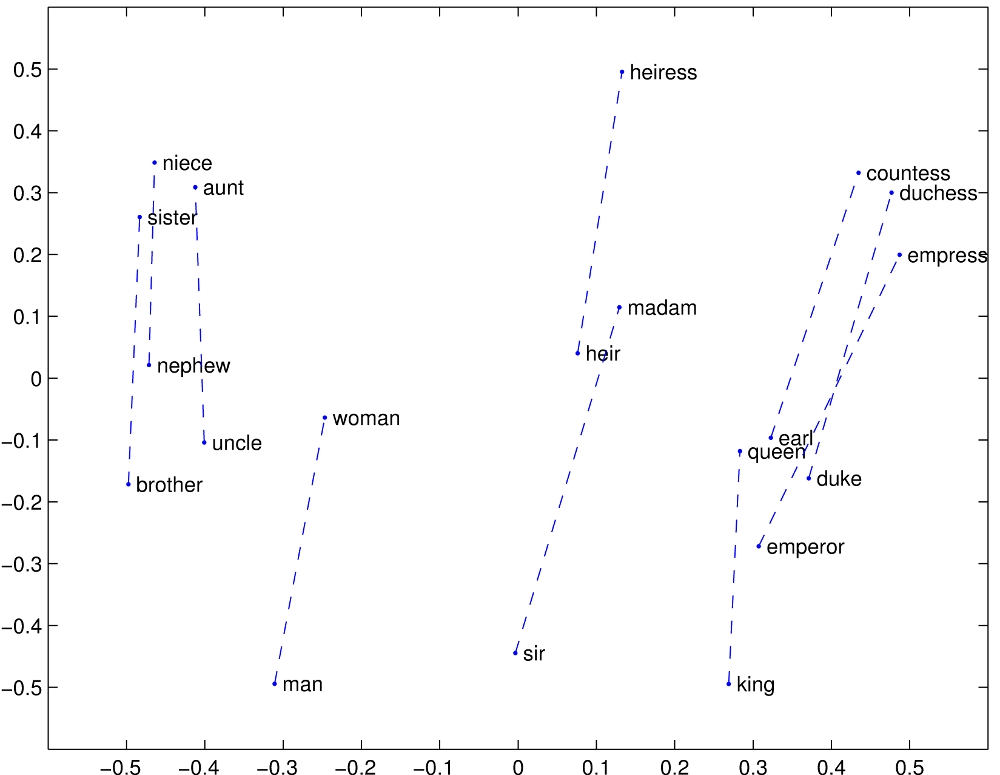
\includegraphics[width = 0.6\textwidth]{glove.jpg}
	\caption[rnn_vanish]{GloVe可视化词向量}
\end{figure}

GloVe结合了基于矩阵分解的词嵌入表示和基于语言模型(例如Word2Vec)的词嵌入表示。基于矩阵分解具有训练快,容易实习的优点,但是生成词向量语义消息十分有限。基于语言模型的词嵌入表示则具有更多语言学层次的支持,在更多自然语言处理任务上表现更好,但是模型关注的上下文特征较少,忽略了全局的信息。GloVe发明的初衷,就是想结合两者的长处,建立一个充分利用统计量的更好训练的适用程度更广的词嵌入模型。具体模型建立公式如下

$$ F(w_i,w_j,w^c_k) = \cfrac{P_{ij}}{P_{jk}} $$
其中,取$word_i$的出现次数为$X_i$, 定义$P_{ij}=P(j|i)=\cfrac{X_{ij}}{X_{i}}$表示在$X_i$的上下文下$word_i$的出现几率, $F$则是某一种能够实现我们需求的变换。$w_i,w_j$是实数空间下的$word_i,,word_j$的词向量,$w^c_k$也是实数空间下的$word_k$的上下文词向量,其作用类似word2vec中的上下文向量。为了精简计算引入词向量的线性加减和点乘计算
$$ F((w_i-w_j)^Tw^c_k) = \cfrac{F(w^T_iw^c_k)}{{F(w^T_jw^c_k)}} $$
GloVe每个词涉及到两个词向量,一个词语本身的向量$w_i$,一个词的context向量$w^c_i$。最初这样设计,将词向量和上下文的向量分开,不用一套,是为了在更新参数的时候能够简单地套用SGD。实验证明两个向量加起来最后起到的效果最好。后面英文的词向量用的是GloVe模型在大量的Twitter文本上训练的100维度的词向量,中文微博词向量是200维度的词向量。

\BiSubsection{长短期记忆神经网络模型}{Layouts of illustrations}
由于文本序列的通常具有较长的长度,导致神经网络的层数较多,而传统的递归神经网络解决序列问题经常会出现梯度消失的问题(vanishing gradient problem)与梯度爆炸问题(gradient exploding problem)。梯度消失问题和梯度爆炸问题一般随着网络层数的增加会变得越来越明显。出现的原因在于对神经网络参数进行链式求导的过程中,输出对于前面递归神经参数的倒数随着累乘激活函数的导数而接近于0,以下图的反向传播为例(假设每一层只有一个神经元且对于每一层$y_i=\sigma(z_i)=\sigma(w_ix_i+b_i)$,其中$\sigma$为sigmoid函数)

\begin{figure}[htbp]
	\centering
	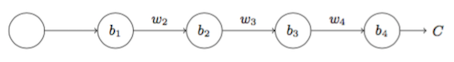
\includegraphics[width = 0.7\textwidth]{rnn_gradient_vanish.png}
	\caption[rnn_vanish]{RNN梯度消失}
\end{figure}

可以推导出

\begin{equation}\label{nodelimiter}
\frac{\partial C}{\partial b_1} = \frac{\partial C}{\partial y_4}\frac{\partial y_4}{\partial z_4}\frac{\partial z_4}{\partial x_4}\frac{\partial x_4}{\partial z_3}\frac{\partial z_3}{\partial x_3}\frac{\partial x_3}{\partial z_2}\frac{\partial z_2}{\partial x_2}\frac{\partial x_2}{\partial z_1}\frac{\partial z_1}{\partial b_1}
\end{equation}
\begin{equation}\label{delimiter}
=\frac{\partial C}{\partial y_4}\ \sigma ^\prime(z_4)w_4\sigma ^\prime(z_3)w_3\sigma ^\prime(z_2)w_2\sigma ^\prime(z_1)
\end{equation}

一般的非线性激活函数的导数都小于1(例如sigmoid的导数最大值为$\frac{1}{4}$),因此对于上面的链式求导,层数越多,求导结果$\frac{\partial C}{\partial b_1}$越小,因而导致梯度消失的情况出现。
长短期记忆(Long Short-Term Memory, LSTM)是一种缓解上述问题的间递归神经网络的变种,Hochreiter在1997年首次提出了LSTM结构,2000年Gers等人改进LSTM模型。

\begin{figure}[htbp]
	\centering
	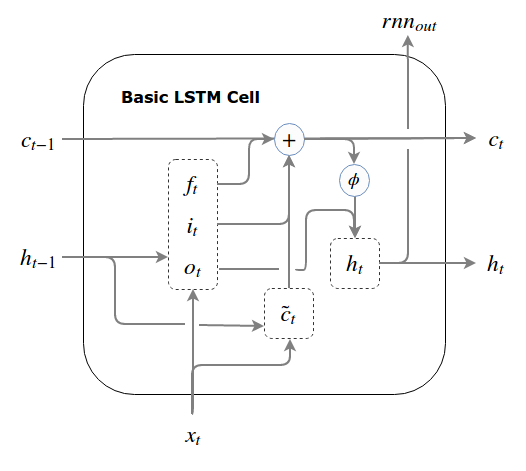
\includegraphics[width = 0.6\textwidth]{lstm_unit.png}
	\caption[rnn_vanish]{LSTM单元结构}
\end{figure}

LSTM模型提出了记忆存储格(memory cell)的结构,内部包含了遗忘门(forget gate)、输入门(input gate) 和输出门(output gata) 。各种门的作用在于调节记忆体在外部输入的情况下应该采取怎么的存储测量,具体门状态和记忆体内部参数的更新公式如下。

\begin{equation}\label{lstm_f}i_t=\sigma_g(W^ix_t+U_ih_{t-1}+b^i)\end{equation}
\begin{equation}\label{lstm_f}f_t=\sigma_g(W^fx_t+U_fh_{t-1}+b^f)\end{equation}
\begin{equation}\label{lstm_f}o_t=\sigma_g(W^ox_t+U_oh_{t-1}+b^o)\end{equation}
\begin{equation}\label{lstm_f}c_t=f_t \odot c_{t-1}+i_t\odot \sigma_c(W_cx_t+U_ch_{t-1}+b_c)\end{equation}
\begin{equation}\label{lstm_f}h_t=o_t \odot \sigma_h(c_t)\end{equation}

其中$\sigma_g$为sigmoid的激活函数,$\sigma_c, \sigma_h$为thah的激活函数,$x_t$为输入向量,$h_t$为输出向量, $c_t$为记忆向量,$W,U,b$是矩阵参数和向量参数。各个门的值是保持在0-1之间的向量。其中遗忘门向量$f_t$表示上一时刻的记忆体信息需要遗忘多少, 输入门向量$i_t$表示有多少当前时刻输入信息需要加入到记忆体中,输出门向量$o_t$表示记忆体输出多少信息。

前已经证明,LSTM是解决长序依赖问题的有效技术,并且这种技术的普适性非常高,导致带来的可能性变化非常多。各研究者根据LSTM纷纷提出了自己的变量版本,这就让LSTM可以处理千变万化的垂直问题

\BiSubsection{条件编码长短期记忆神经网络模型}{}
Rocktaschel[]等在句子之间的文本蕴含识别的研究中提出了条件编码长短期记忆神经网络模型,文本蕴含定义为一对文本之间的有向推理关系,其中蕴含前件记作T(Text),蕴含后件记作H(Hypothesis)。如果人们依据自己的常识认为H的语义能够由T的语义推理得出的话,那么称T蕴含H,记作T → H, 作者提出的模型的结构是首先有一个LSTM模型编码Text消息,另一个不同参数的LSTM模型编码Hypothesis。作者不是简单把两个特征向量拼接在一起,而是做了如下转换。把第一个编码Text信息的LSTM模型的记忆状态(Cell)保留下来,作为第二个编码Hypothesis的LSTM模型记忆状态(Cell)的初始值,此模型建立的了Text消息作为条件下的对Hypothesis的编码表示。

\begin{figure}[htbp]
	\centering
	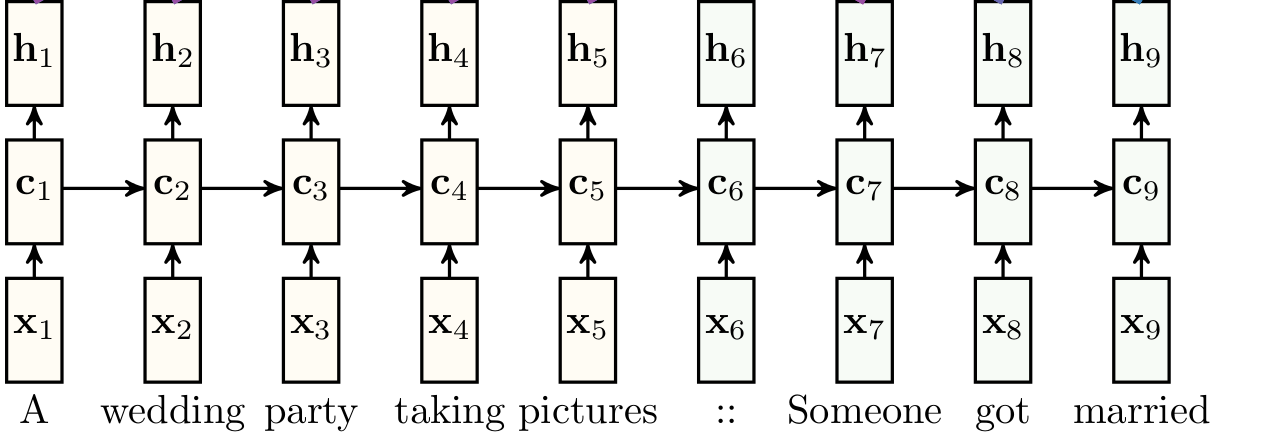
\includegraphics[width = 0.8\textwidth]{conditional_encoding.png}
	\caption[rnn_vanish]{条件编码长短期记忆}
\end{figure}

如上图图表示所示“A wedding party taking pictures”作为我们的Text文本,“Someone got married”作为我们的Hypothesis,其中$c_5$作为前一个LSTM的记忆体状态被当做编码Hypothesis的初始记忆状态。两个LSTM具体的状态转移公式如下:
\begin{equation}\label{lstm_f}[h_1~c_1] = LSTM^{Text}(x_1,h_0,c_0)\end{equation}
$$...$$
\begin{equation}\label{lstm_f}[h_T~c_T] = LSTM^{Text}(x_1,h_{T-1},c_{T-1})\end{equation}
\begin{equation}\label{lstm_f}[h_{T+1}~c_{T+1}] = LSTM^{Hypothesis}(x_1,h_0,c_T)\end{equation}
$$...$$
\begin{equation}\label{lstm_f}[h_{N}~c_{N}] = LSTM^{Hypothesis}(x_1,h_{N-1},c_{N-1})\end{equation}
\begin{equation}\label{lstm_f}c=tanh(Wh_N)\end{equation}
其中$(x_1...x_T)$为Text的序列消息,$(x_{T+1}...x_N)$为Hypothesis的序列信息。$h_0,c_0$为LSTM的初始化向量。

实验证明在文本蕴含任务上,条件LSTM模型比单独编码高3.3\%(从77.6\%提升到80.9\%)的性能。这种条件编码能使Text的信息更好的流向对Hypothesis编码的LSTM模型,有了第一个LSTM模型传来的记忆状态,第二个LSTM模型能更好的编码Hypothesis的消息。

\BiSection{基于条件编码长短期记忆的文本立场分析}{}

通过Rocktaschel在文本蕴含的任务的实验可知,在处理两个文本序列的编码任务上,条件编码长短期记忆神经网络比单独独立编码两个文本序列有更好的建模能力。在文本立场分析的任务上,有文本的信息和目标主题两个文本序列信息,我们可以借鉴条件编码长短期记忆神经网络在文本蕴含建模的方式,把文本信息和目标主题信息更好结合起来。在实验部分设计了多种文本序列信息的结合方式,通过实验证明了以目标主题文本作为条件编码文本信息的模型对文本立场分析有更好的效果。

本文后期实验将在NLPCC2016中文微博立场分析数据集和SemEval2016英文Twitter立场分析数据集,为较清晰阐述条件编码长短期记忆模型,以下简短的介绍下两个数据集的样例,具体的有关数据集的信息将会在下面实验部分做详细介绍。

例1:目标主题文本:"深圳禁摩限电" 微博文本:"支持深圳交警。电单车继续治理" 立场分析类标:“Favor”(持支持立场)

目标的文本主题有关“深圳禁摩限电”的主题的,而从微博文本“支持深圳交警。电单车继续治理”中,我们可以知道微博的作者首先是赞同了深圳交警的行为,然后叙述了电单车需要得到继续的整治,从两个方法肯定了"深圳禁摩限电"这个主题目标的,因此给出的类标是“Favor”也就是持支持目标主题的立场。

例1:目标主题文本:"Hillary Clinton" Twitter文本:"Hopefully Hillary Clinton gets cancer and dies before she gets the opportunity to embarrass our country any further“,立场分析类标“Against”(持反对立场)

译文:"真希望希拉里克林顿得癌症然后死去,这样她就不再会有机会再让我们国家蒙羞了。"

目标的文本主题有关“希拉里克林顿”的主题的,这个Twitter文本是有关2016年美国大选,显然Twitter作者一直咒骂希拉里克林顿,希望她得癌症,不让她侮辱国家,可以看出作者有强烈反对主题目标“希拉里克林顿”,因此给出的类标是“Against”,也就是持反对目标主题的立场。

从上述的两个简单的样例可知,立本立场是有两个输入的,一个是立场主题例如“深圳禁摩限电”和“Hillary Clinton”。另外一个是立场下的文本“支持深圳交警。电单车继续治理”和”Hopefully Hillary Clinton gets cancer and dies before she gets the opportunity to embarrass our country any further“。在这通过中文微博阐述条件编码长短期记忆模型的建立。首先经过一些数据预处理和分词把主题目标”深圳禁摩限电“和”支持深圳交警。电单车继续治理”转变成”深圳 禁摩 限电“和”支持 深圳 交警 电单车 继续 治理“。

在文本立场分析的任务, 一般目标主题包含的信息较少,而文本包含了大部分的信息。例如上面两个例子所举例的,目标主题文本分别为”Hillary Clinton“和”深圳禁摩限电“,而Twitter和微博文本包含的消息较多,结合立场分析文本的特点,改善了原有的条件编码长短期记忆的网络结构,后续实验论证在多种条件编码长短期记忆的改进方案中,下面所示的网络结构具有更好的实验效果,后续在实验分析其可能的原因。

\begin{figure}[htbp]
	\centering
	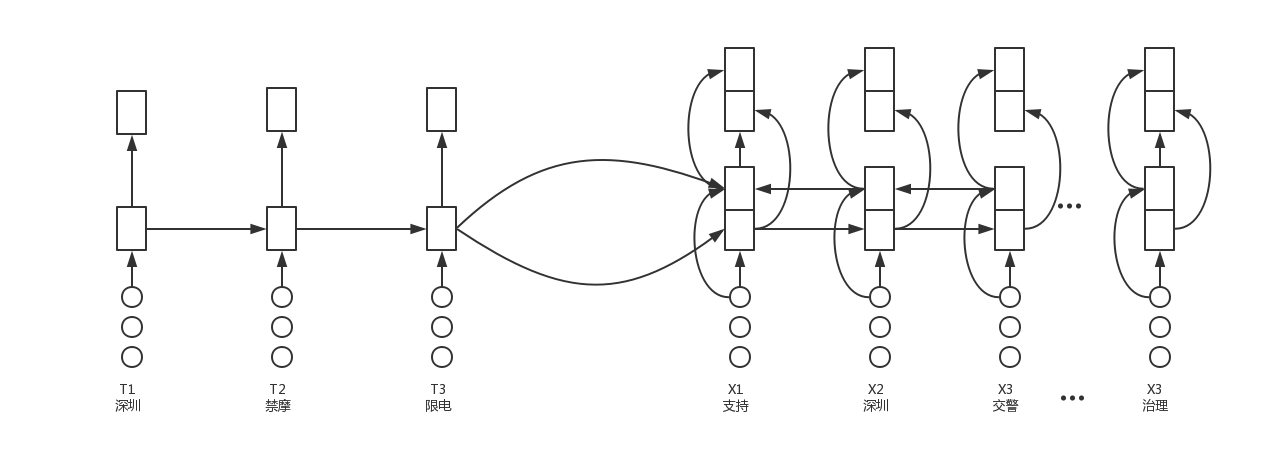
\includegraphics[width = 1.0\textwidth]{conditional_encode_lstm.png}
	\caption[rnn_vanish]{条件编码长短期记忆}
\end{figure}

模型的具体公式如下

\begin{equation}\label{lstm_f}[h_1~c_1] = LSTM^{target}(t_1,h_0,c_0)\end{equation}
$$...$$
\begin{equation}\label{lstm_f}[h_M~c_M] = LSTM^{target}(t_1,h_{M-1},c_{M-1})\end{equation}

\begin{equation}\label{lstm_f}[h^{forward}_{1}~c^{forward}_{1}] = LSTM^{forward}(x_1,h_0,c_T)\end{equation}
$$...$$
\begin{equation}\label{lstm_f}[h^{forward}_{N}~c^{forward}_{N}] = LSTM^{forward}(x_n,h^{forward}_{N-1},c^{forward}_{N-1})\end{equation}

\begin{equation}\label{lstm_f}[h^{backward}_{N}~c^{backward}_{N}] = LSTM^{backward}(x_n,h_0,c_T)\end{equation}
$$...$$
\begin{equation}\label{lstm_f}[h^{backward}_{1}~c^{backward}_{1}] = LSTM^{backward}(x_1,h^{backward}_{2},c^{backward}_{2})\end{equation}

\begin{equation}\label{lstm_f}c_i=Softmax(W[h^{forward}_n~h^{backward}_1])\end{equation}

其中$M$为主题目标的文本长度,$N$为微博()Twiiter的文本长度。$LSTM$单向编码主题目标,$LSTM^{forward}$为前向编码文本信息,$LSTM^{backward}$为后向编码文本信息,$h_0$为LSTM的初始化向量,$C_T$为$LSTM$主题目标编码的最后一个Cell状态,$h^{backward}_{1},h^{forward}_{N}$分别为前向和后向编码的最后一个隐藏状态。

本节以“深圳禁摩限电”为话题目标,微博文本“支持深圳交警。电单车继续治理”为例,按本节模型的5个层次,描述基于条件编码长短期记忆的立场分析的过程。

(1)输入层

先将话题目标和微博文本经过预处理操作,然后通过分词工具把话题目标和微博文本进行划分,对于同一个话题目标,微博文本分词后句子长度有可能不一致,为了方便后续神经网络框架中的批量的并行计算,通过统计选择30为固定长度,长度超过固定长度进行截断操作,不够的进行补齐词表中规定<PAD>关键词。如例微博文本最后转换成”支持 深圳 交警。电单车 继续 治理 <PAD> ... <PAD>“

(2)词向量嵌入层

词向量的嵌入层,此层的功能是对输入的每一次词检索其词向量(lookup操作),后续实验词向量的预训练由GloVe模型在大量无监督语料上训练可得,预训练的词向量维度为100,且把词向量设置为可训练,随神经网络模型的训练动态调整权重。

(3)主题目标编码层

通过一个单向的长短期记忆(LSTM)模型模型编码主题目标,把分词后的主题目标“深圳 禁摩 限电”通过lookup操作取出相应的词向量,经过一个隐藏层为64的单向LSTM模型,且保留最后的记忆体的状态,如上图所示,保留XXX的单元的信息,给下一层文本编码做输入。

(4)文本编码层

由于文本包含大部分信息,所以采用了双向的LSTM模型而不是Rocktaschel提出的单向的LSTM模型编码文本信息。如上图所示,文本编码的双向LSTM模型的初始Cell状态是由上一层的目标主题编码的最后的Cell状态填充,表示主题目标的消息流入到当前的双向LSTM模型中参与对文本的编码操作。每一个方向LSTM的最后的隐状态h作为对整个文本的最终编码表示。

(5)全连接层


全连接层接受来自文本编码层每个方向最后的隐状态,拼接两个隐状态信息作为最后的特征向量。全连接层的输出个数为3,表示每个立场的预测概率。通过softmax激活函数归一化三个立场的概率,在预测阶段我们选取概率最大的立场当做预测的类标。

\BiSection{实验结果及分析}{hello}

本节主要介绍条件编码长短期记忆神经网络模在2016NLPCC微博中文语料库和2016SemEval英文Twitter数据集中的实验结果及分析。并从实验的角度论证条件编码长短期记忆在立场分析问题上的有效性。本节包含两部分: 3.4.1 小节介绍中英文两个数据集中训练和测试文本的分布 、实验评价方式以及对比方法;3.4.2 小结介绍模型训练阶段的性能调优,以及本章实验与其他方法的比较。

\BiSubsection{实验数据与评价指标}{}

(1)数据集简介

为验证条件编码长短期记忆神经网络在立场分析任务上算法的性能表现,本节采用2016 NLPCC中文微博语料和2016 SemEval英文的Twitter语料两个数据集验证算法的效果。以下分别介绍两数据集的分布。

中文数据集来自NLPCC2016 立场分析测评任务[55] ,数据集的5个话题目标分别为 iPhone SE、春节放鞭炮、俄罗斯在叙利亚的反恐行动、开放二胎政策和深圳禁摩限电。所有语料都来自于新浪微博,每个微博文本的立场属于“支持”、“反对”和“其他”三者之一。NLPCC 2016中文微博数据集的训练集、测试集按照75\%与25\%的比例划分,如表~\ref{chinesedata}~所示详细介绍每个话题目标下数据的分布。
\begin{table}[htbp]
	\caption[table123]{训练集、测试集话题数量及立场分布比例(中文数据集)}
	\label{chinesedata}
	\vspace{0.5em}\centering\wuhao
	\begin{tabular}{cccccccccc}
		\toprule[1.5pt]
		\multirow{2}{*}{预置话题分类}& \multicolumn{4}{c}{训练集数量和立场比例(\%)} 
		& \multicolumn{4}{c}{测试集数量和立场比例(\%)}  &\multirow{2}{*}{文本数量}\\
		\cline{2-9}
		\quad&数量& 支持&反对&其他&数量& 支持&反对&其他 \\
		\midrule[1pt]
		iPhone SE&600&40.8&34.8&24.3&200&37.5&52.0&10.5&800\\
		春节放鞭炮&600&41.7&41.7&16.7&200&44.0&47.0&9.0&800\\
		俄在叙反恐行动&600&41.7&41.7&16.7&200&47.0&43.0&10.0&800\\
		开放二胎政策&600&43.3&33.3&23.3&200&49.5&47.5&3.0&800\\
		深圳禁摩限电&600&26.7&50.0&23.3&200&31.5&55.0&13.5&800\\
		总计&3000&38.8&40.3&20.9&1000&41.9&48.9&9.2&4000\\
		\bottomrule[1.5pt]
	\end{tabular}
\end{table}

英文数据集来自SemEval2016 Task6 stance detection[55] ,数据集的5个话题目标分别为 Atheism(无神论)、Climate Change is a Real Concern(气候变化真实性)、Feminist Movement(女权运动)、 Hillary Clinton (希拉里克林顿)和
Legalization of Abortion(堕胎合法化)。所有语料都来自于英文Twitter文本,每个Twitter文本的立场属于“支持”、“反对”和“其他”三者之一。不同于上述中文语料的分布,每个话题目标英文Twitter语料的数量参差不齐,但总体上训练集和测试集按70\%与30\%的比例划分,如表~\ref{englishdata}~所示详细介绍每个话题目标下数据的分布。


\begin{table}[htbp]
	\caption[table123]{训练集、测试集话题数量及立场分布比例(英文数据集)}
	\label{englishdata}
	\vspace{0.5em}\centering\wuhao
	\begin{tabular}{cccccccccc}
		\toprule[1.5pt]
		\multirow{2}{*}{预置话题分类}& \multicolumn{4}{c}{训练集数量和立场比例(\%)} 
		& \multicolumn{4}{c}{测试集数量和立场比例(\%)}  &\multirow{2}{*}{文本数量}\\
		\cline{2-9}
		\quad&数量& 支持&反对&其他&数量& 支持&反对&其他 \\
		\midrule[1pt]
		Atheism&513&17.9&59.3&22.8&220&14.5&72.7&12.7&733\\
		Climate Change&395&53.7&3.8&42.5&169&72.8&6.5&20.7&564\\
		Feminist Movement&664&31.6&49.4&19.0&285&20.4&64.2&15.4&949\\
		Hillary Cliton&689&17.1&57.0&25.8&295&15.3&58.3&26.4&984\\
		Legal of Abortion&653&18.5&54.4&27.1&280&16.4&67.5&16.1&933\\
		总计&2914&25.8&47.9&26.3&1249&24.3&57.3&18.4&4163\\
		\bottomrule[1.5pt]
	\end{tabular}
\end{table}

为了和已有方法进行性能比较,本文在两数据集上都按照分别测评的比例划分出训练集和测试集。其中训练集负责模型的训练和调优, 测试集则进行最后模型的性能的评估。中英文数据集均包含5个不同的话题目标, 每个话题目标包含若干的话题文本,由于每个主题目标关注的内容不同且具有各自独特的语言特点。为了使模型更好的拟合每一种话题的特性,本文首先按照中英文不同语料集合划分成两个大任务,然后根据每个语料库在细分成5个不同子任务,分别建立不同的条件编码长短期记忆模型。各子模型预测结束后, 统计各个子任务上的性能并汇总预测结果进行最后统一指标的计算。

(2)评价指标

中英文数据集上的社交媒体文本的立场结果有“支持”,“反对”,“其他”,可以把任务当成一个三分类任务,但是由于三个类在不同的数据集下的不同主题目标的分布有可能很不平均,如果只单独用正确率(Accuracy)作为评测指标则缺失了评价指标的客观性。本文c采取了两个评测任务都使用的”支持“和”反对“的F1指标的微平均(micro-average)作为最后模型的评测指标,但是为了更清晰的评价每个主题目标的性能,每个目标主题也会单独计算微平均评测指标。为了清晰地解释指标的含义,列举以下公式说明

首先定义准确率(Precision, P)、召回率(Recall, R),如公式~\ref{precision}~和公式~\ref{recall}~所示。
\begin{equation}\label{precision}P=\frac{TP}{TP+FP}\end{equation}
\begin{equation}\label{recall}F=\frac{TP}{TP+FN}\end{equation}

TP:正样例预测为正样例的个数

FP:负样例预测为正样例的个数

FN:正样例预测为负样例的个数。

精确率计算的是所有"正确被检索的样例(TP)"占所有"实际被检索到的(TP+FP)样例的比例。召回率计算的是所有"正确被检索的运力(TP)"占所有"应该检索到的样例(TP+FN)"的比例。如果要同时考虑精确率和召回率,则需要采样两者的调和平均值,也称为F1值,其定义如公式~\ref{f1score}~所示
\begin{equation}\label{f1score}F1=\frac{2PR}{P+R}=\frac{2TP}{2TP+FP+FN}\end{equation}

有关”支持“立场F1值的计算,“支持”类标作为正样本,“反对”后“其他”作为负样本。因此其计算公式如下所示

\begin{equation}\label{f1favor}F1_{favor}=\frac{2P_{favor}R_{favor}}{P_{favor}+R_{favor}}\end{equation}

同样的”反对“立场F1值的计算,“反对”类标作为正样本,“支持”后“其他”作为负样本。因此其计算公式如下所示

\begin{equation}\label{f1against}F1_{against}=\frac{2P_{against}R_{against}}{P_{against}+R_{against}}\end{equation}

立场分析总的平均指标F1的微平均(Micro-average)的计算公式如下
\begin{equation}\label{f1average}F1_{average}=\frac{F1_{favor}+F1_{against}}{2}\end{equation}

为论证在立场分析中,合理利用主题目标的信息能提高立场分析的性能,设计了以下模型。

用LSTM直接编码文本Text信息,不引入主题目标信息,以下简称\textbf{Text-Only}。

用两个不同LSTM模型分别编码主题目标Target和文本Text信息,两个LSTM独立编码各自的信息,最后拼接两者的编码向量作为最后参与分类的特征向量,以下简称\textbf{Text-Target}。

用两个不同LSTM模型分别编码主题目标Target和文本Text信息,对主题目标Target最后LSTM模型的记忆单元(Cell)状态做为对文本编码LSTM模型的初始状态,构成以主题目标Target为条件的Text文本编码,取Text编码LSTM的最后一个隐状态作为最后的特征向量,以下简称\textbf{Text-on-Target}。

针对立场分析数据的特点,主题目标所包含的信息相对有限,而文本包含绝大部分信息的特点。改进了条件编码的模型,与(3)相同用单向的LSTM编码主题目标信息,为了充分提取文本的信息,采用双向LSTM模型来提取文本的信息,类似于(3)的做法,编码文本的双向LSTM模型的记忆单元来自于对主题目标编码的LSTM的最后记忆单元状态,以下简称\textbf{BiText-on-Target}。

首先为了初步验证主题目标的信息对立场分析是否具有提升作用,通过对比Text-Only和Text-Target模型的性能可以初步得出主题目标的信息对立场分析是否有促进作用,然后为了进一步说明条件编码LSTM模型是否能跟好的利用主题目标的消息参与对文本的编码,设计了Text-Target模型和Text-on-Target模型的对比实验。最后为了对比我们改进过了的条件编码BiText-on-Target模型是否能更好编码文本信息,设计了Text-on-Target模型和BiText-on-Target模型的对比实验。

\BiSubsection{实验数据预处理与模型参数设计}{}

本文实验的社交媒体立场分析数据都来自于新浪微博或者Twitter,此类网络语言文本具有文本形式极度不规范,口语化严重。Twitter与微博是由网络用户即兴创作的短文本,用户在用词、语法等方面随意性较大,文本形式与新闻、维基百科等语料具有很大的差异。由于Twitter和微博一般有对单条文本长度做出文本长度的限制,因此这些网络文本中常含有缩写、俗语、流行词汇等元素,同样也存在语法成分缺失的问题。除此之外,文本中大量存在的网页链接、“@某用户”和“\#某话题”等功能标记。

由于社交媒体文本根据上述特点,分别对中英文语句进行预处理操作。删除语料中其中的大量URL信息,由于“\#某话题”等话题标签对立场分析有很重要的影响,因此把话题标签消息保留了下来,对于英文所有词语全转换成小写拼写,分词工具采用了CMU专门为Twitter开发的Twitter NLP tool里面的分词模型[XXX], 中文的分词工具采用较为稳定的结巴分词工具。对于网络社交文本分词后可转换成一些词语的序列信息,对于在训练集中出现次数小于2词的词语归为低频词,为了减少模型的参数,加大模型的泛化能力,把所以的低频词转换成一个统一的词汇用“UNKNOW”标识。同时为了兼容现在主流的基于批量更新的深度学习框架,对文本的长度进行固定操作。英文的文本固定为30个词的长度,中文微博文本固定为50的词长度。

英文语料的词向量训练通过GloVe算法在20亿Twitter文本语料训练而成,其中包含了120万个词,词向量维度为200。中文微博语料是通过Word2Vec算法在大量微博语料中训练所得,其中包含了17万个词,词向量的维度也为200。

本文建立了针对5个不同话题目标的子模型, 使用相同的条件编码长短期记忆模型参数。取出训练集合的10\%作为验证集参与模型的选择。通过实验发现,当对主题目标和文本编码LSTM模型的隐藏层单元设置为64,embedding层的dropout的概率设置为0.2,当对主题目标和文本编码LSTM模型内部记忆的dropout概率设置为0.3,每次以32个样本作为mini-batch参加参数更新,选取0.001的学习率的Adam优化方法。

\begin{table}[htbp]
	\caption[param]{基于条件双向编码长短期记忆的立场分析实验超参数集}
	\label{param}
	\vspace{0.5em}\centering\wuhao
	\begin{tabular}{ccc}
		\toprule[1.5pt]
		序号& 超参数名称 &数值\\
		\midrule[1pt]
		1 &LSTM隐藏层单元& 64\\
		2 &Embedding层dropout& 0.2\\
		3 &LSTM内部drought& 0.3\\
		4 &批处理大小& 32\\
		5 &L2 正则化参数 &1e-6\\
		6 &全量迭代次数& 50\\
		7 &梯度优化方法& Adam\\
		8 &学习率& 0.001\\
		\bottomrule[1.5pt]
	\end{tabular}
\end{table}

\BiSubsection{模型对比实验结果及分析}{}
通过在
\begin{table}[htbp]
	\caption[table123]{基于子话题分别训练的条件双向编码长短期记忆模型试验性能(SemEval数据集)}
	\label{chinesedata}
	\vspace{0.5em}\centering\wuhao
	\begin{tabular}{cccccccc}
		\toprule[1.5pt]
		预置话题分类& $P_{favor}$&$R_{favor}$&$F_{favor}$&$P_{against}$&$R_{against}$&$F_{against}$&$F_{average}$ \\
		\midrule[1pt]
		iPhone SE&600&40.8&34.8&24.3&200&37.5&52.0\\
		春节放鞭炮&600&41.7&41.7&16.7&200&44.0&47.0\\
		俄在叙反恐行动&600&41.7&41.7&16.7&200&47.0&43.0\\
		开放二胎政策&600&43.3&33.3&23.3&200&49.5&47.5\\
		深圳禁摩限电&600&26.7&50.0&23.3&200&31.5&55.0\\
		总计&3000&38.8&40.3&20.9&1000&41.9&48.9\\
		\bottomrule[1.5pt]
	\end{tabular}
\end{table}

\begin{table}[htbp]
	\caption[table123]{基于子话题分别训练的条件双向编码长短期记忆模型试验性能(NLPCC数据集)}
	\label{chinesedata}
	\vspace{0.5em}\centering\wuhao
	\begin{tabular}{cccccccc}
		\toprule[1.5pt]
		预置话题分类& $P_{favor}$&$R_{favor}$&$F_{favor}$&$P_{against}$&$R_{against}$&$F_{against}$&$F_{average}$ \\
		\midrule[1pt]
		iPhone SE&600&40.8&34.8&24.3&200&37.5&52.0\\
		春节放鞭炮&600&41.7&41.7&16.7&200&44.0&47.0\\
		俄在叙反恐行动&600&41.7&41.7&16.7&200&47.0&43.0\\
		开放二胎政策&600&43.3&33.3&23.3&200&49.5&47.5\\
		深圳禁摩限电&600&26.7&50.0&23.3&200&31.5&55.0\\
		总计&3000&38.8&40.3&20.9&1000&41.9&48.9\\
		\bottomrule[1.5pt]
	\end{tabular}
\end{table}


% !Mode:: "TeX:UTF-8" 

\BiChapter{图片的插入方法}{Methods of inserting figures}

\BiSection{研究生院的插图规范}{Figures inserting standard from graduate school}
图应有自明性。插图应与文字紧密配合,文图相符,内容正确。选图要力求精练,插图、照片应完整清晰。图中文字和数字等字号用宋体~5~号字。

机械工程图:采用第一角投影法,严格按照~GB4457---GB131-83《机械制图》标准规定。

数据流程图、程序流程图、系统流程图等按~GB1526-89~标准规定。

电气图:图形符号、文字符号等应符合附录~3~所列有关标准的规定。

流程图:必须采用结构化程序并正确运用流程框图。

对无规定符号的图形应采用该行业的常用画法。

坐标图的坐标线均用细实线,粗细不得超过图中曲线,有数字标注的坐标图,必须注明坐标单位。

照片图要求主题和主要显示部分的轮廓鲜明,便于制版。如用放大或缩小的复制品,必须清晰,反差适中。照片上应有表示目的物尺寸的标度。

引用文献图表必须标注出处。


\BiSubsection{图题及图中说明}{Captions and descriptions of figures}
每个图均应有图题(由图序和图名组成),图名在图序之后空一格排写。图序按章编排,如第~1~章第一个插图的图号为“图~1-1”等。
图题置于图下,硕士论文可只用中文书写,博士论文用中、英文两种文字居中书写,中文在上,要求中文用宋体~5~号字,英文用~Times New Roman 5~号字。有图注或其它说明时应置于图题之上。引用图应注明出处,在图题右上角加引用文献号。
图中若有分图时,分图题置于分图之下或图题之下,分图号用~a)、b)等表示。

图中各部分说明应采用中文(引用的外文图除外)或数字项号,各项文字说明置于图题之上(有分图题者,置于分图题之上)。

\BiSubsection{插图编排}{Layouts of illustrations}
插图之前,文中必须有关于本插图的提示,如“见图~1-1”、“如图~1-1~所示”等。插图与其图题为一个整体,不得拆开排写于两页。
插图处的该页空白不够排写该图整体时,则可将其后文字部分提前排写,将图移到次页。

\BiSection{\LaTeX~中推荐使用的图片格式}{Recommended figure format applied in \LaTeX}
在~\LaTeX~中应用最多的图片格式是~EPS(Encapsulated PostScript)格式,它是一种专用的打印机描述语言,常用于印刷或打印输出。
EPS~格式图片可通过多种方式生成,这里介绍一款功能强大的免费图片处理软件———\href{http://www.imagemagick.org/}{ImageMagick},
360~软件管家也提供此软件的下载。此软件可将其它格式图片转换为~EPS~格式图片,同时还可以锐化图片,使图片的局部清晰一些。

此软件对图片的格式转换操作都是在命令提示符(cmd.exe)中实现的,可以通过“开始$\to$运行$\to$输入~cmd$\to$回车”或
“开始$\to$程序$\to$附件$\to$命令提示符”找到它。在命令提示符下,首先采用“盘符命令”或“cd~命令”将当前目录改为待处理图片所在的目录,
在此目录下就可通过~convert~命令将图片转换为~EPS~格式,其命令的语法格式为

\noindent\verb|convert [可选参数] 原文件名.原扩展名 新文件名.eps|

\noindent 若~convert~命令中无可选参数,则将原来的图片格式直接转换为~EPS~格式,对图片不进行任何处理,这也是最常用的方法。
也可以选用可选参数,可选参数有很多选择,但最常用的有如下两个:

\verb|-sharpen radius{xsigma}|———此参数用来锐化图片,一般用在图片像素不高,需要提高图片清晰度的情况下。其中~radius~只能为整数,
它用来确定转换命令采取哪一种锐化算法,我们可以只取~radius~为~0;sigma~为所采取算法的锐化度,它的取值为~0.1--3~之间的任意一个浮点数,
数值越大,锐化程度也越大,通常取为~0.5--1~之间;x在参数中为分隔符。

\verb|-resize geometry|———此参数用来改变图片的大小,若图片的存储空间过大,可通过此命令缩小图片尺寸,但同时也将导致图片像素降低,
其具体用法请参见\href{http://www.imagemagick.org/script/command-line-options.php#resize}{-resize geometry的官方说明}。

除此之外,一些文字处理软件和科学计算软件也支持生成~EPS~格式的文件,请使用“另存为”功能查看某款软件是否能够将图片以~EPS~格式的形式保存。

\BiSection{单张图片的插入方法}{The method of inserting one single figure}
单张图片独自占一行的插入形式如图~\ref{golfer1}~所示。
\begin{figure}[htbp]
\centering
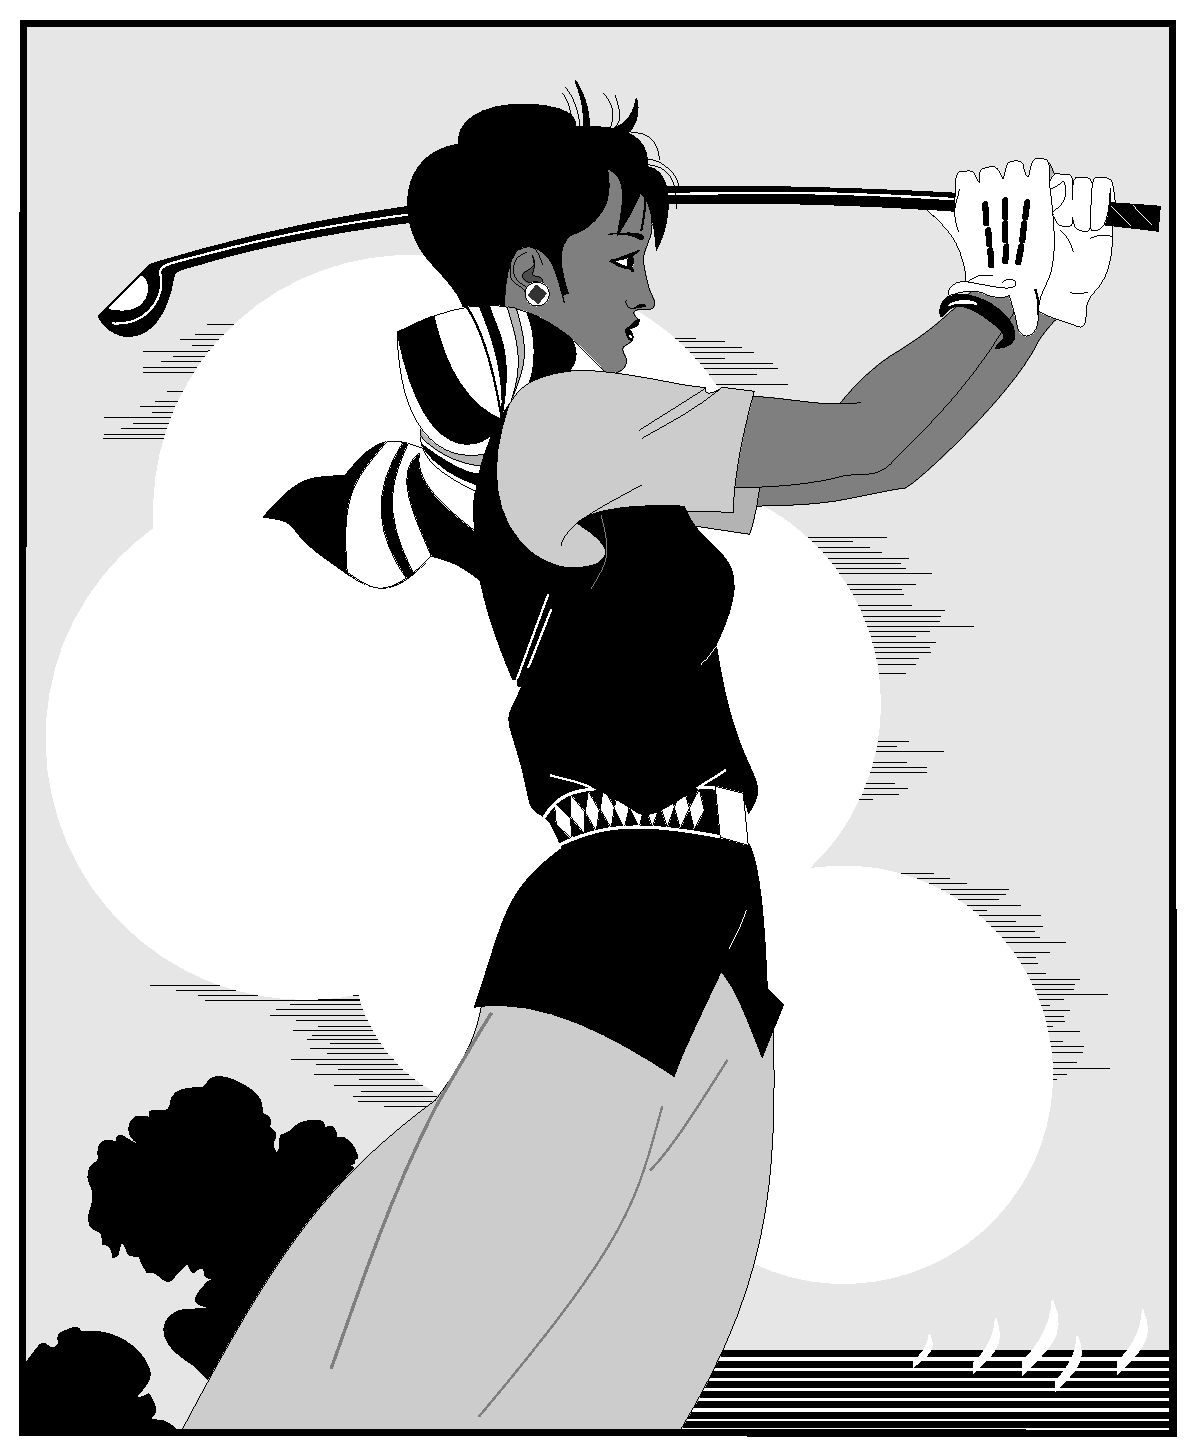
\includegraphics[width = 0.4\textwidth]{golfer}
\bicaption[golfer1]{}{打高尔夫球的人}{Fig.$\!$}{The person playing golf}\vspace{-1em}
\end{figure}

其插入图片的代码及其说明如下。
\vspace{1em}\noindent\hrule
\begin{lstlisting}
\begin{figure}[htbp]
\centering
\includegraphics[width=0.4\textwidth]{文件名(.eps)}
\bicaption[标签名(英文)]{}{中文标题}{Fig.$\!$}
          {English caption (首字母大写)}\vspace{-1em}
\end{figure}
\end{lstlisting}
\noindent\hrule
\begin{lstlisting}
figure环境的可选参数[htbp]表示浮动图形所放置的位置,h (here)表示当前位置,t (top)表示页芯顶部,b (bottom)表示页芯底部,p (page)表示单独一页。在word等软件中,图片通常插入到当前位置,如果当前页的剩余空间不够,图片将被移动到下一页,当前页就会出现很大的空白,其人工调整工作非常不便。由LaTeX提供的浮动图片功能,总是会按h->t->b->p的次序处理选项中的字母,自动调整图片的位置,大大减轻了工作量。
\centering命令将后续内容转换成每行皆居中的格式。
“\includegraphics”的可选参数用来设置图片插入文中的水平宽度,一般表示为正文宽度(\textwidth)的倍数。
\bicaption命令的使用需要调用ccaption宏包,它可以为图片或表格插入双语标题(博士学位论文要求),可选参数“标签名”为英文形式,一般不以图片或表格的数字顺序作为标签,而应包含一定的图片或表格信息,以便于文中引用(若图片、表格、公式、章节和参考文献等在文中出现的先后顺序发生了变化,其标注序号及其文中引用序号也会跟着发生变化,这一点是word等软件所不能做到的)。第4个参数中的“$\!$”表示-1/6个空铅宽度,这样可以缩小Fig.和Table与后面数字序号之间的水平距离。另外,图题或表题并不会因为分页而与图片或表格体分置于两页,章节等各级标题也不会置于某页的最底部,LaTeX系统会自动调整它们在正文中的位置,这也是word等软件所无法匹敌的。
注:硕士学位论文的图表只需要插入中文标题,因此需将\bicaption一句命令替换为如下两条命令(下同):
\caption{中文标题}
\label{标签名(英文)}
\vspace将产生一定高度的竖直空白,必选参数为负值表示将后续文字位置向上提升,参数值可自行调整。em为长度单位,相当于大写字母M的宽度。
引用方法:“见图~\ref{标签名(英文)}”、“如图~\ref{标签名(英文)}~所示”等。
\end{lstlisting}
\noindent\hrule\vspace{1em}
若需要将~2~张及以上的图片并排插入到一行中,则需要采用\verb|minipage|环境,如图~\ref{golfer2}~和图~\ref{golfer3}~所示。
\begin{figure}[htbp]
\centering
\begin{minipage}{0.4\textwidth}
\centering
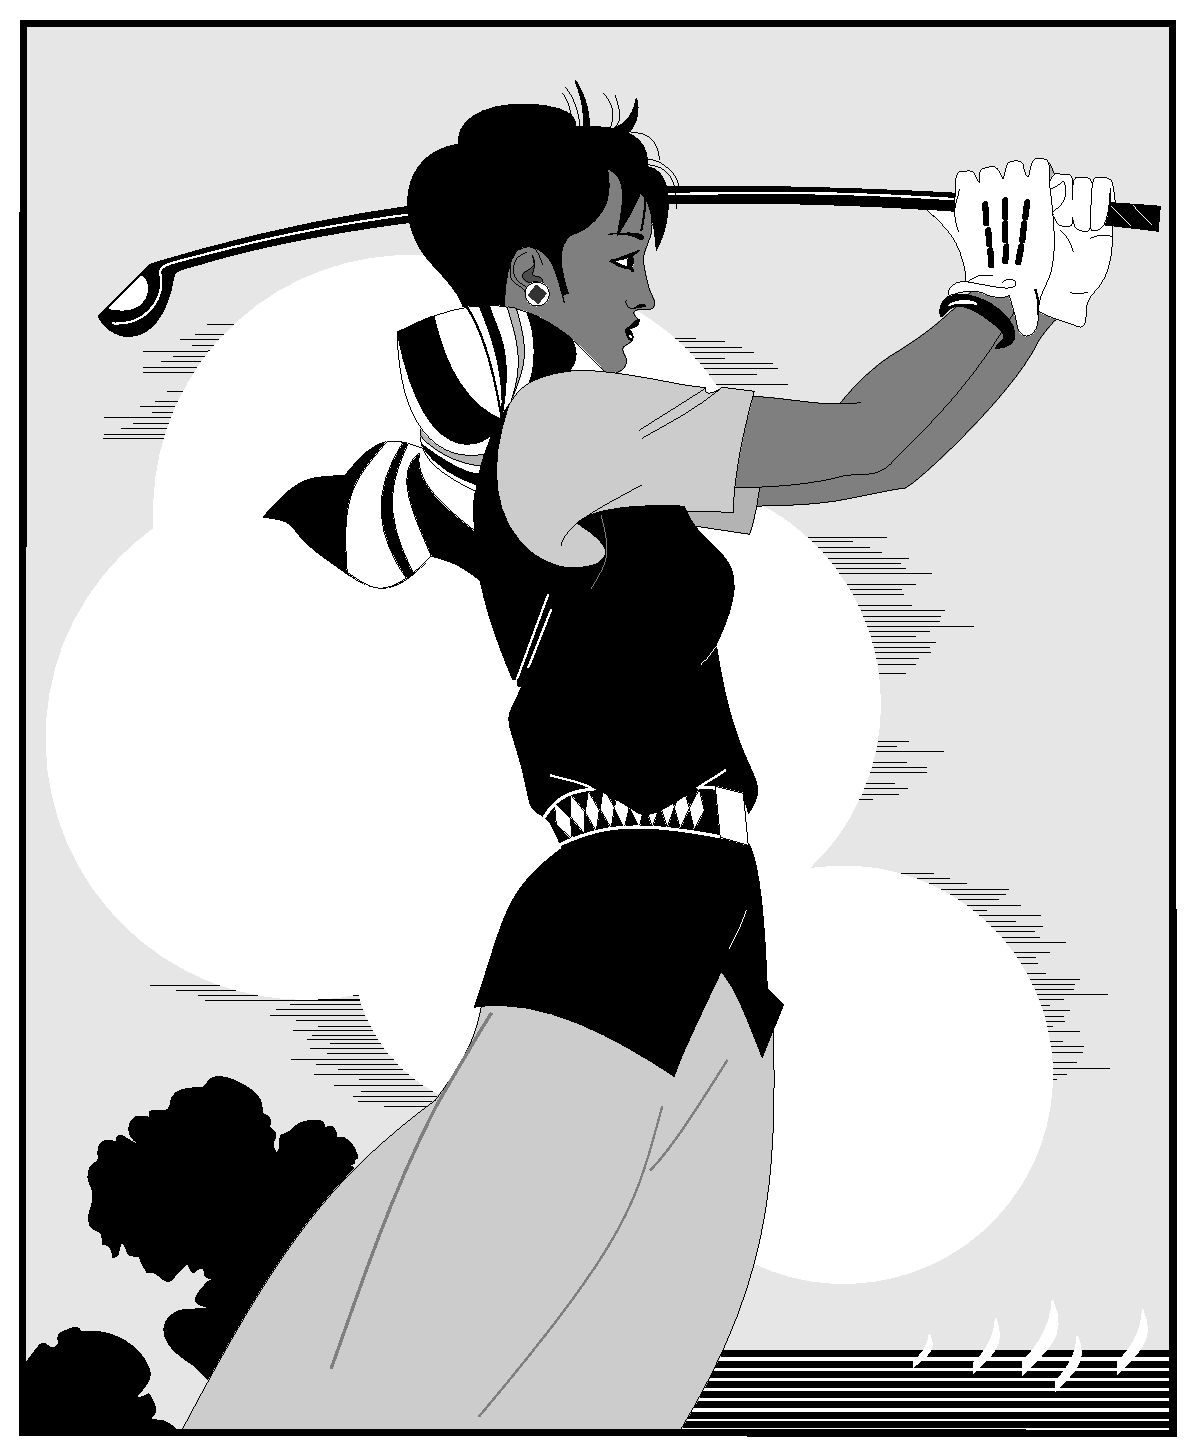
\includegraphics[width=\textwidth]{golfer}
\bicaption[golfer2]{}{打高尔夫球的人}{Fig.$\!$}{The person playing golf}
\end{minipage}
\begin{minipage}{0.4\textwidth}
\centering
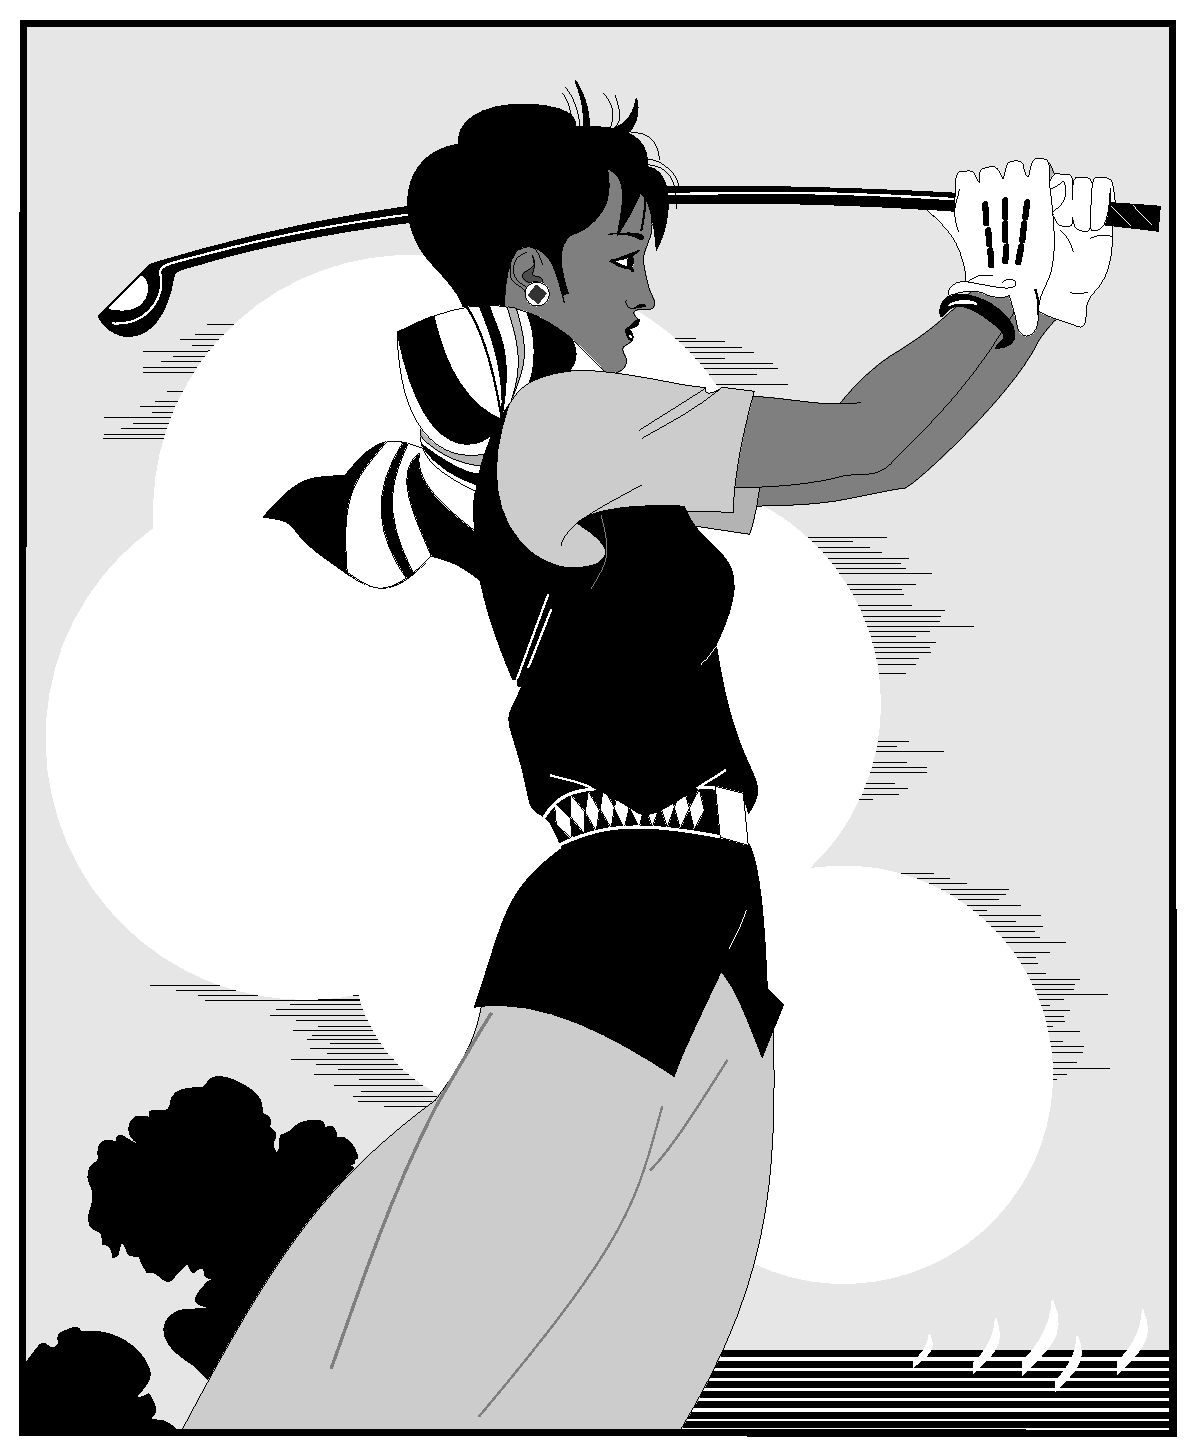
\includegraphics[width=\textwidth]{golfer}
\bicaption[golfer3]{}{打高尔夫球的人}{Fig.$\!$}{The person playing golf}
\end{minipage}\vspace{-1em}
\end{figure}

其代码如下所示。
\vspace{1em}\noindent\hrule
\begin{lstlisting}
\begin{figure}[htbp]
\centering
\begin{minipage}{0.4\textwidth}
\centering
\includegraphics[width=\textwidth]{文件名}
\bicaption[标签名]{}{中文标题}{Fig.$\!$}
          {English caption}
\end{minipage}
\begin{minipage}{0.4\textwidth}
\centering
\includegraphics[width=\textwidth]{文件名}
\bicaption[标签名]{}{中文标题}{Fig.$\!$}
          {English caption}
\end{minipage}\vspace{-1em}
\end{figure}
\end{lstlisting}
\noindent\hrule
\begin{lstlisting}
minipage环境的必选参数用来设置小页的宽度,若需要在一行中插入n个等宽图片,则每个小页的宽度应略小于(1/n)\textwidth。
\end{lstlisting}
\noindent\hrule

\BiSection{具有子图的图片插入方法}{The method of inserting figures with subfigures}

图中若含有子图时,需要调用~subfigure~宏包。博士学位论文规范要求不止总图的标题为中英文形式,其各个子图也应具有中英文形式的标题。
然而~ccaption~宏包却无法实现子图的中英文标题功能,这里采用对\verb|\subfigure|命令进行嵌套的方法来实现子图的中英文标题功能,如图~\ref{golfer4}~所示。

\begin{figure}[htbp]
\centering
\subfigure{\label{golfer41}}\addtocounter{subfigure}{-2}
\subfigure[The person playing golf]{\subfigure[打高尔夫球的人~1]{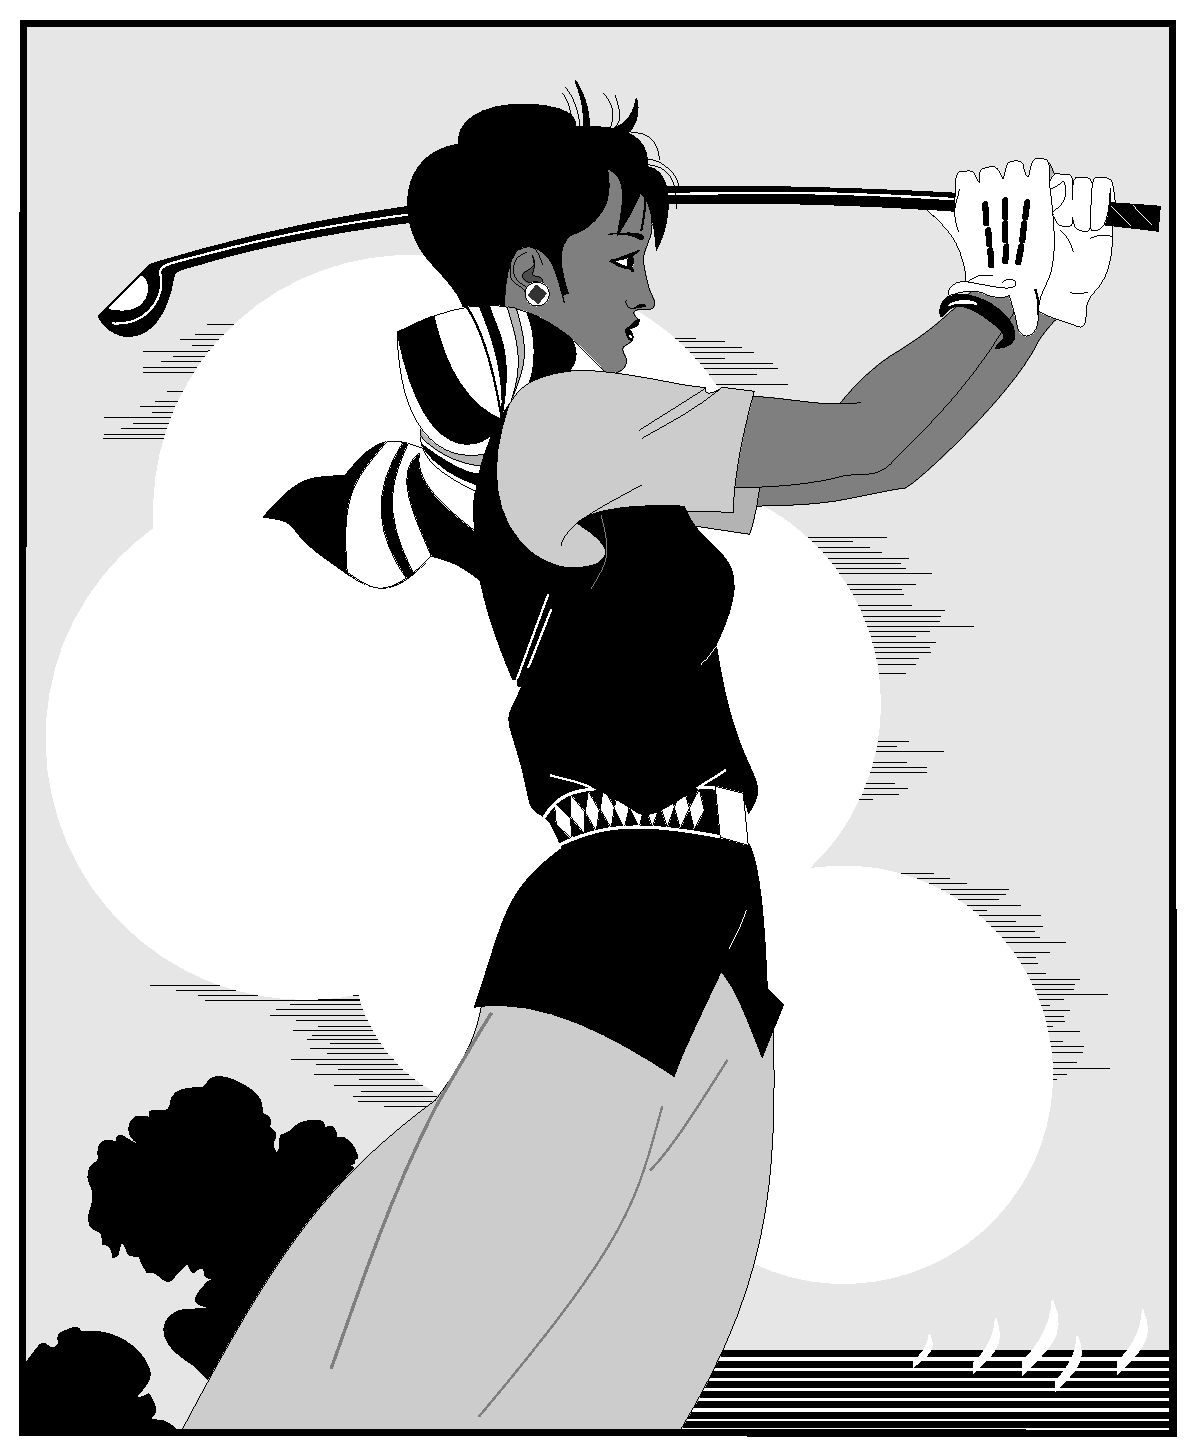
\includegraphics[width=0.4\textwidth]{golfer}}}
\subfigure{\label{golfer42}}\addtocounter{subfigure}{-2}
\subfigure[The person playing golf]{\subfigure[打高尔夫球的人~2]{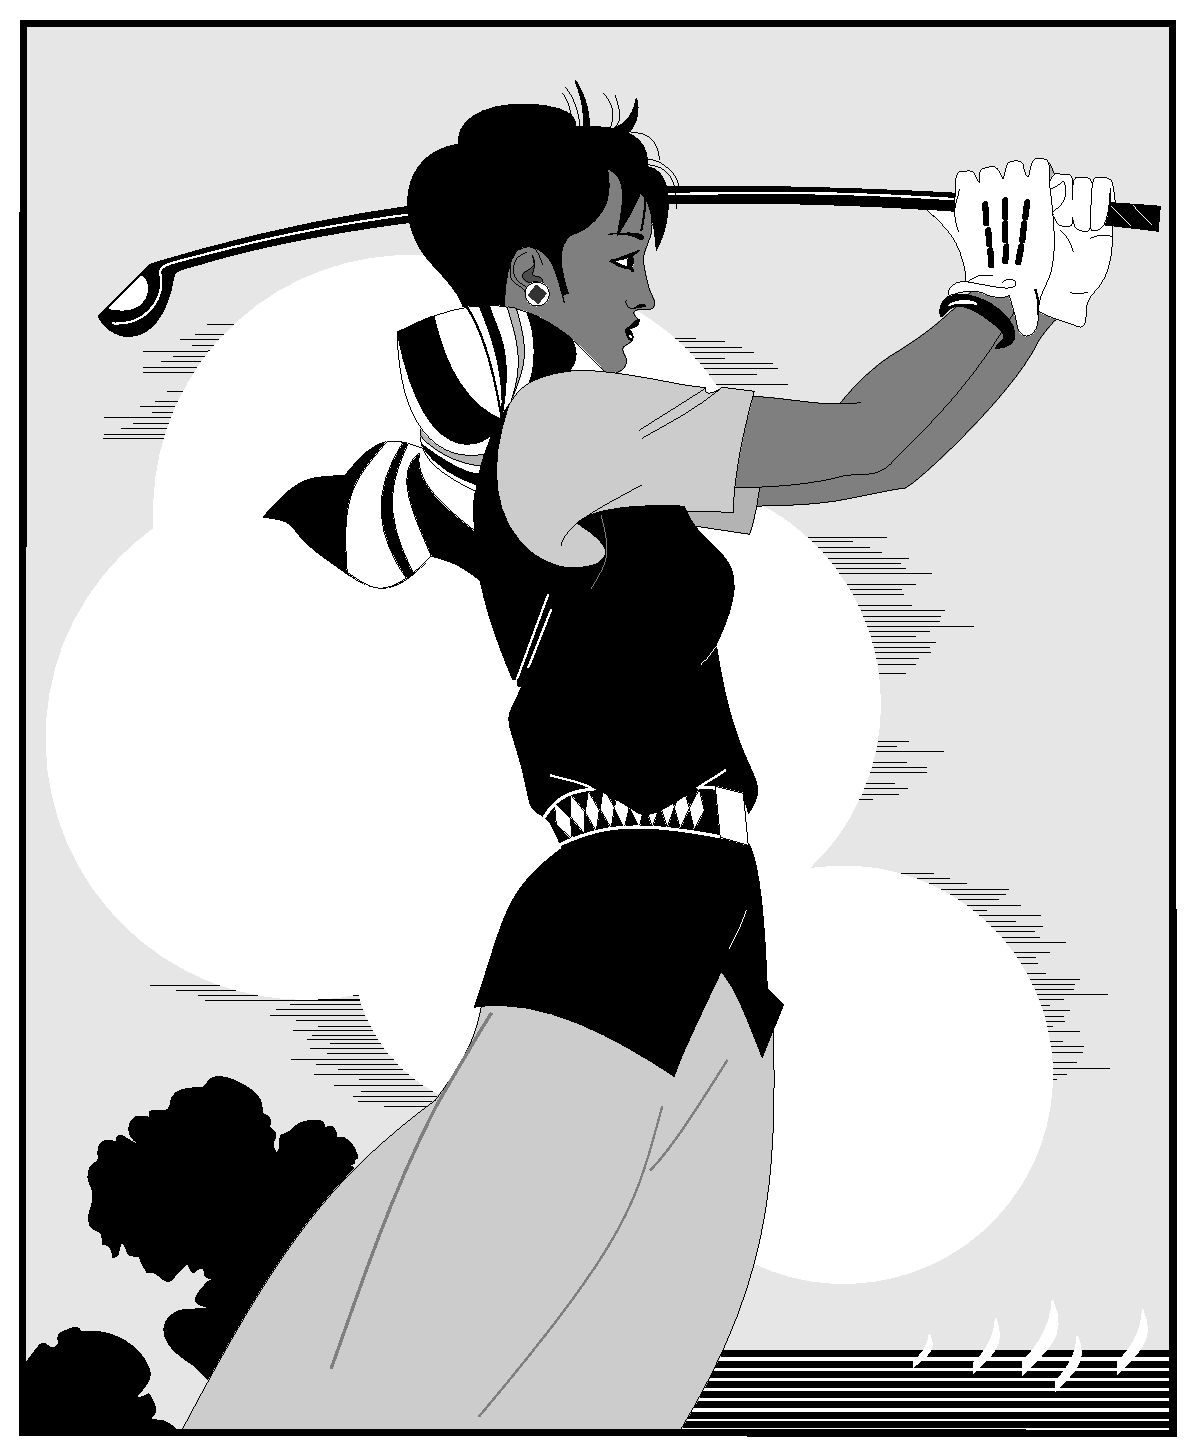
\includegraphics[width=0.4\textwidth]{golfer}}}
\bicaption[golfer4]{}{打高尔夫球的人}{Fig.$\!$}{The person playing golf}\vspace{-1em}
\end{figure}

其代码及其说明如下。
\vspace{1em}\noindent\hrule
\begin{lstlisting}
\begin{figure}[htbp]
\centering
\subfigure{\label{第1个子图标签名}}\addtocounter{subfigure}{-2}
\subfigure[The 1st subfigure caption]{\subfigure[第1个子图标题]
          {\includegraphics[width=0.4\textwidth]{文件名}}}
\subfigure{\label{第2个子图标签名}}\addtocounter{subfigure}{-2}
\subfigure[The 2nd subfigure caption]{\subfigure[第2个子图标题]
          {\includegraphics[width=0.4\textwidth]{文件名}}}
\bicaption[总标签名]{}{中文总标题}{Fig.$\!$}{The total caption}
\vspace{-1em}
\end{figure}
\end{lstlisting}
\noindent\hrule
\begin{lstlisting}
\addtocounter把指定的值加到计数器上,这里是对subfigure计数器进行减2操作。这是因为每插入1个子图,就调用3次\subfigure命令,第1次调用\subfigure命令用来生成紧随其后所插入子图的标签,而之后的双层嵌套调用\subfigure命令用来插入子图并生成该子图的中英文标题。因此,每插入1张子图,subfigure计数器的值就自动加3,为了使得子图的序号能每次加1,则需在每插入1张子图前手动把subfigure计数器的值减2。
\subfigure命令的双层嵌套使用可用来生成中英文标题,其内层\subfigure命令用来插入子图并生成中文标题,外层\subfigure命令将插入的子图和中文标题作为一个整体,生成这个整体的英文标题,因此英文标题会置于中文标题的下面。
硕士学位论文只需要中文标题,其代码如下:
\begin{figure}[htbp]
\centering
\subfigure[第1个子图标题\label{第1个子图标签名}]
          {\includegraphics[width=0.4\textwidth]{文件名}}
\subfigure[第2个子图标题\label{第2个子图标签名}]
          {\includegraphics[width=0.4\textwidth]{文件名}}
\caption{中文总标题}\label{总标签名}
\vspace{-1em}
\end{figure}
引用方法:总图的引用方法同本章第1节,子图的引用方法用\ref{第n个子图标签名}来代替。
\end{lstlisting}
\noindent\hrule\vspace{1em}

子图的引用示例:如图~\ref{golfer41}~和图~\ref{golfer42}~所示。

若想获得插图方法的更多信息,请参见网络上的~\href{ftp://ftp.tex.ac.uk/tex-archive/info/epslatex.pdf}{Using Imported Graphics in \LaTeX and pdf\LaTeX}~文档。 

% !Mode:: "TeX:UTF-8" 

\BiChapter{表格的绘制方法}{Methods of drawing tables}
\BiSection{研究生院的绘表规范}{Tables drawing standard from graduate school}

表应有自明性。表格不加左、右边线。表的编排建议采用国际通行的三线表。表中文字用宋体~5~号字。

每个表格均应有表题(由表序和表名组成)。表序一般按章编排,如第~1~章第一个插表的序号为“表~1-1”等。表序与表名之间空一格,
表名中不允许使用标点符号,表名后不加标点。表题置于表上,硕士学位论文只用中文,博士学位论文用中、英文两种文字居中排写,
中文在上,要求中文用宋体~5~号字,英文用新罗马字体~5~号字。

表头设计应简单明了,尽量不用斜线。表头中可采用化学符号或物理量符号。

全表如用同一单位,则将单位符号移至表头右上角,加圆括号。
表中数据应准确无误,书写清楚。数字空缺的格内加横线“-”(占~2~个数字宽度)。表内文字或数字上、下或左、右相同时,
采用通栏处理方式,不允许用“〃”、“同上”之类的写法。

表内文字说明,起行空一格、转行顶格、句末不加标点。

如某个表需要转页接排,在随后的各页上应重复表的编号。编号后加“(续表)”,表题可省略。续表应重复表头。

\BiSection{普通表格的绘制方法}{Methods of drawing normal tables}

表格应具有三线表格式,因此需要调用~booktabs~宏包,其标准格式如表~\ref{table1}~所示。
\begin{table}[htbp]
\bicaption[table1]{}{符合研究生院绘图规范的表格}{Table$\!$}{Table in agreement of the standard from graduate school}
\vspace{0.5em}\centering\wuhao
\begin{tabular}{ccccc}
\toprule[1.5pt]
$D$(in) & $P_u$(lbs) & $u_u$(in) & $\beta$ & $G_f$(psi.in)\\
\midrule[1pt]
 5 & 269.8 & 0.000674 & 1.79 & 0.04089\\
10 & 421.0 & 0.001035 & 3.59 & 0.04089\\
20 & 640.2 & 0.001565 & 7.18 & 0.04089\\
\bottomrule[1.5pt]
\end{tabular}
\end{table}

其绘制表格的代码及其说明如下。
\vspace{1em}\noindent\hrule
\begin{lstlisting}
\begin{table}[htbp]
\bicaption[标签名]{}{中文标题}{Table$\!$}{English caption}
\vspace{0.5em}\centering\wuhao
\begin{tabular}{cc...c}
\toprule[1.5pt]
表头第1个格   & 表头第2个格   & ... & 表头第n个格  \\
\midrule[1pt]
表中数据(1,1) & 表中数据(1,2) & ... & 表中数据(1,n)\\
表中数据(2,1) & 表中数据(2,2) & ... & 表中数据(2,n)\\
...................................................\\
表中数据(m,1) & 表中数据(m,2) & ... & 表中数据(m,n)\\
\bottomrule[1.5pt]
\end{tabular}
\end{table}
\end{lstlisting}
\noindent\hrule
\begin{lstlisting}
table环境是一个将表格嵌入文本的浮动环境。
\wuhao命令将表格的字号设置为五号字(10.5pt),在绘制表格结束退出时,不需要将字号再改回为\xiaosi,正文字号默认为小四号字(12pt)。
tabular环境的必选参数由每列对应一个格式字符所组成:c表示居中,l表示左对齐,r表示右对齐,其总个数应与表的列数相同。此外,@{文本}可以出现在任意两个上述的列格式之间,其中的文本将被插入每一行的同一位置。表格的各行以\\分隔,同一行的各列则以&分隔。
\toprule、\midrule和\bottomrule三个命令是由booktabs宏包提供的,其中\toprule和\bottomrule分别用来绘制表格的第一条(表格最顶部)和第三条(表格最底部)水平线,\midrule用来绘制第二条(表头之下)水平线,且第一条和第三条水平线的线宽为1.5pt,第二条水平线的线宽为1pt。
引用方法:“如表~\ref{标签名}~所示”。
\end{lstlisting}
\noindent\hrule

\BiSection{长表格的绘制方法}{Methods of drawing long tables}

长表格是当表格在当前页排不下而需要转页接排的情况下所采用的一种表格环境。若长表格仍按照普通表格的绘制方法来获得,
其所使用的\verb|table|浮动环境无法实现表格的换页接排功能,表格下方过长部分会排在表格第1页的页脚以下。为了能够实现长表格的转页接排功能,
需要调用~longtable~宏包,由于长表格是跨页的文本内容,因此只需要单独的\verb|longtable|环境,所绘制的长表格的格式如表~\ref{table2}~所示。

此长表格~\ref{table2}~第~2~页的标题“编号(续表)”和表头是通过代码自动添加上去的,无需人工添加,若表格在页面中的竖直位置发生了变化,长表格在第~2~页
及之后各页的标题和表头位置能够始终处于各页的最顶部,也无需人工调整,\LaTeX~系统的这一优点是~word~等软件所无法比拟的。

\wuhao\begin{longtable}{ccc}
\longbionenumcaption{}{中国省级行政单位一览\label{table2}}{Table$\!$}{}{Overview of the provincial administrative unit of China} \vspace{0.5em}\\
\toprule[1.5pt] 名称 & 简称 & 省会或首府  \\ \midrule[1pt]
\endfirsthead
\multicolumn{3}{r}{表~\thetable(续表)}\vspace{0.5em}\\
\toprule[1.5pt] 名称 & 简称 & 省会或首府  \\ \midrule[1pt]
\endhead
\bottomrule[1.5pt]
\endfoot
北京市 & 京 & 北京\\
天津市 & 津 & 天津\\
河北省 & 冀 & 石家庄市\\
山西省 & 晋 & 太原市\\
内蒙古自治区 & 蒙 & 呼和浩特市\\
辽宁省 & 辽 & 沈阳市\\
吉林省 & 吉 & 长春市\\
黑龙江省 & 黑 & 哈尔滨市\\
上海市 & 沪/申 & 上海\\
江苏省 & 苏 & 南京市\\
浙江省 & 浙 & 杭州市\\
安徽省 & 皖 & 合肥市\\
福建省 & 闽 & 福州市\\
江西省 & 赣 & 南昌市\\
山东省 & 鲁 & 济南市\\
河南省 & 豫 & 郑州市\\
湖北省 & 鄂 & 武汉市\\
湖南省 & 湘 & 长沙市\\
广东省 & 粤 & 广州市\\
广西壮族自治区 & 桂 & 南宁市\\
海南省 & 琼 & 海口市\\
重庆市 & 渝 & 重庆\\
四川省 & 川/蜀 & 成都市\\
贵州省 & 黔/贵 & 贵阳市\\
云南省 & 云/滇 & 昆明市\\
西藏自治区 & 藏 & 拉萨市\\
陕西省 & 陕/秦 & 西安市\\
甘肃省 & 甘/陇 & 兰州市\\
青海省 & 青 & 西宁市\\
宁夏回族自治区 & 宁 & 银川市\\
新疆维吾尔自治区 & 新 & 乌鲁木齐市\\
香港特别行政区 & 港 & 香港\\
澳门特别行政区 & 澳 & 澳门\\
台湾省 & 台 & 台北市\\
\end{longtable}\xiaosi

绘制长表格的代码及其说明如下。
\vspace{1em}\noindent\hrule
\begin{lstlisting}

\wuhao\begin{longtable}{cc...c}
\longbionenumcaption{}{中文标题\label{标签名}}{Table$\!$}
                    {}{English caption}\vspace{0.5em}\\
\toprule[1.5pt] 表头第1个格 & 表头第2个格 & ... & 表头第n个格\\ \midrule[1pt]
\endfirsthead
\multicolumn{n}{r}{表~\thetable(续表)}\vspace{0.5em}\\
\toprule[1.5pt] 表头第1个格 & 表头第2个格 & ... & 表头第n个格\\ \midrule[1pt]
\endhead
\bottomrule[1.5pt]
\endfoot
表中数据(1,1) & 表中数据(1,2) & ... & 表中数据(1,n)\\
表中数据(2,1) & 表中数据(2,2) & ... & 表中数据(2,n)\\
...................................................\\
表中数据(m,1) & 表中数据(m,2) & ... & 表中数据(m,n)\\
\end{longtable}\xiaosi
\end{lstlisting}
\noindent\hrule
\begin{lstlisting}
在绘制长表格的前面留出一个空白行,并在第2行的一开始全局定义长表格的字号为五号字,这样能够保证长表格之前段落的行距保持不变。在绘制长表格结束后,需要\xiaosi命令重新将字号改为小四号字。
长表格的中英文标题是通过ccaption宏包的\longbionenumcaption命令得到的。
\endhead之前的文字描述的是第2页及其之后各页的标题或表头;\endfirsthead之前的文字描述的是第1页的标题和表头,若无此命令,则第1页的表头和标题由\endhead命令确定;同理,\endfoot之前的文字描述的是除最后一页之外每页的表格底部内容;\endlastfoot之前的文字描述的是最后一页的表格底部内容,若无此命令,则最后一页的表格底部内容由\endfoot命令确定;由于规范中长表格每页底部内容均相同(水平粗线),因此模板中没有用到\endlastfoot命令。
注:硕士学位论文的长表格只需要插入中文标题,因此需将\longbionenumcaption一句命令替换为如下两条命令 :
\caption{中文标题}
\label{标签名}
\end{lstlisting}
\noindent\hrule

\BiSection{列宽可调表格的绘制方法}{Methods of drawing tables with adjustable-width columns}
论文中能用到列宽可调表格的情况共有两种,一种是当插入的表格某一单元格内容过长以至于一行放不下的情况,
另一种是当对公式中首次出现的物理量符号进行注释的情况,这两种情况都需要调用~tabularx~宏包。下面将分别对这两种情况下可调表格的绘制方法进行阐述。
\BiSubsection{表格内某单元格内容过长的情况}{The condition when the contents in some cells of tables are too long}
首先给出这种情况下的一个例子如表~\ref{table3}~所示。
\begin{table}[htbp]
  \centering
\bicaption[table3]{}{最小的三个正整数的英文表示法}{Table$\!$}{The English construction of the smallest three positive integral numbers}\vspace{0.5em}\wuhao
\begin{tabularx}{0.7\textwidth}{llX}
\toprule[1.5pt]
Value & Name & Alternate names, and names for sets of the given size\\\midrule[1pt]
1 & One & ace, single, singleton, unary, unit, unity\\
2 & Two & binary, brace, couple, couplet, distich, deuce, double, doubleton, duad, duality, duet, duo, dyad, pair, snake eyes, span, twain, twosome, yoke\\
3 & Three & deuce-ace, leash, set, tercet, ternary, ternion, terzetto, threesome, tierce, trey, triad, trine, trinity, trio, triplet, troika, hat-trick\\\bottomrule[1.5pt]
\end{tabularx}
\end{table}

绘制这种表格的代码及其说明如下。
\vspace{1em}\noindent\hrule
\begin{lstlisting}
\begin{table}[htbp]
\bicaption[标签名]{}{中文标题}{Table$\!$}{English caption}
\vspace{0.5em}\wuhao
\begin{tabularx}{\textwidth}{l...X...l}
\toprule[1.5pt]
表头第1个格   & ... & 表头第X个格   & ... & 表头第n个格  \\
\midrule[1pt]
表中数据(1,1) & ... & 表中数据(1,X) & ... & 表中数据(1,n)\\
表中数据(2,1) & ... & 表中数据(2,X) & ... & 表中数据(2,n)\\
.........................................................\\
表中数据(m,1) & ... & 表中数据(m,X) & ... & 表中数据(m,n)\\
\bottomrule[1.5pt]
\end{tabularx}
\end{table}
\end{lstlisting}
\noindent\hrule

\begin{lstlisting}

tabularx环境共有两个必选参数:第1个参数用来确定表格的总宽度,这里取为排版表格能达到的最大宽度——正文宽度\textwidth;第2个参数用来确定每列格式,其中标为X的项表示该列的宽度可调,其宽度值由表格总宽度确定。
标为X的列一般选为单元格内容过长而无法置于一行的列,这样使得该列内容能够根据表格总宽度自动分行。若列格式中存在不止一个X项,则这些标为X的列的列宽相同,因此,一般不将内容较短的列设为X。
标为X的列均为左对齐,因此其余列一般选为l(左对齐),这样可使得表格美观,但也可以选为c或r。

\end{lstlisting}

\noindent\hrule

\BiSubsection{对物理量符号进行注释的情况}{The condition when physical symbols need to be annotated}

为使得对公式中物理量符号注释的转行与破折号“———”后第一个字对齐,此处最好采用表格环境。此表格无任何线条,左对齐,
且在破折号处对齐,一共有“式中”二字、物理量符号和注释三列,表格的总宽度可选为文本宽度,因此应该采用\verb|tabularx|环境。
由\verb|tabularx|环境生成的对公式中物理量符号进行注释的公式如式(\ref{eq:1})所示。

\begin{equation}\label{eq:1}
\ddot{\boldsymbol{\rho}}-\frac{\mu}{R_{t}^{3}}\left(3\mathbf{R_{t}}\frac{\mathbf{R_{t}\rho}}{R_{t}^{2}}-\boldsymbol{\rho}\right)=\mathbf{a}
\end{equation}
\begin{tabularx}{\textwidth}{@{}l@{\quad}r@{———}X@{}}
式中& $\boldsymbol{\rho}$ &追踪飞行器与目标飞行器之间的相对位置矢量;\\
&  $\boldsymbol{\ddot{\rho}}$&追踪飞行器与目标飞行器之间的相对加速度;\\
&  $\mathbf{a}$   &推力所产生的加速度;\\
&  $\mathbf{R_t}$ & 目标飞行器在惯性坐标系中的位置矢量;\\
&  $\omega_{t}$ & 目标飞行器的轨道角速度;\\
&  $\mathbf{g}$ & 重力加速度,$=\frac{\mu}{R_{t}^{3}}\left(
3\mathbf{R_{t}}\frac{\mathbf{R_{t}\rho}}{R_{t}^{2}}-\boldsymbol{\rho}\right)=\omega_{t}^{2}\frac{R_{t}}{p}\left(
3\mathbf{R_{t}}\frac{\mathbf{R_{t}\rho}}{R_{t}^{2}}-\boldsymbol{\rho}\right)$,这里~$p$~是目标飞行器的轨道半通径。
\end{tabularx}\vspace{\wordsep}

其中生成注释部分的代码及其说明如下。
\vspace{1em}\noindent\hrule
\begin{lstlisting}
\begin{tabularx}{\textwidth}{@{}l@{\quad}r@{— — —}X@{}}
式中 & symbol-1 & symbol-1的注释内容;\\
     & symbol-2 & symbol-2的注释内容;\\
     .............................;\\
     & symbol-m & symbol-m的注释内容。
\end{tabularx}\vspace{\wordsep}
\end{lstlisting}
\noindent\hrule
\begin{lstlisting}
tabularx环境的第1个参数选为正文宽度,第2个参数里面各个符号的意义为:
    第1个@{}表示在“式中”二字左侧不插入任何文本,“式中”二字能够在正文中左对齐,若无此项,则“式中”二字左侧会留出一定的空白;
    @{\quad}表示在“式中”和物理量符号间插入一个空铅宽度的空白;
    @{— — —}实现插入破折号的功能,它由三个1/2的中文破折号构成;
    第2个@{}表示在注释内容靠近正文右边界的地方能够实现右对齐。
\end{lstlisting}
\noindent\hrule\vspace{1em}
由此方法生成的注释内容应紧邻待注释公式并置于其下方,因此不能将代码放入\verb|table|浮动环境中。但此方法不能实现自动转页接排,
可能会在当前页剩余空间不够时,全部移动到下一页而导致当前页出现很大空白。因此在需要转页处理时,还请您手动将需要转页的代码放入一个
新的\verb|tabularx|环境中,将原来的一个\verb|tabularx|环境拆分为两个\verb|tabularx|环境。

若想获得绘制表格的更多信息,请参见网络上的~\href{http://www.tug.org/pracjourn/2007-1/mori/}{Tables in \LaTeXe: Packages and Methods}~文档。 

% !Mode:: "TeX:UTF-8" 

\BiChapter{数学公式的输入方法}{Input methods of equations}
\BiSection{研究生院的公式规范}{Equations typesetting standard from graduate school}
论文中的公式应另起行,原则上应居中书写,与周围文字留有足够的空间区分开。
若公式前有文字(如“解”、“假定”等),文字空两格写,公式仍居中写。公式末不加标点。

公式应标注序号,并将序号置于括号内。 公式序号按章编排,如第~1~章第一个公式序号为“(1-1)”。公式的序号右端对齐。

公式较长时最好在等号“=”处转行,如难实现,则可在~$+$、$-$、$\times$、$\div$~运算符号处转行,转行时运算符号仅书写于转行式前,不重复书写。

文中引用公式时,一般用“见式~(1-1)”或“由公式~(1-1)”。

公式中用斜线表示“除”的关系时应采用括号,以免含糊不清,如~$a/(b\cos x)$。通常“乘”的关系在前,如~$a\cos x/b$而不写成~$(a/b)\cos x$。

不能用文字形式表示等式,如:$\textnormal{刚度}=\frac{{\textnormal{受力}}}{{\textnormal{受力方向的位移}}}$。

\textbf{对于数学公式的输入方法,网络上有一个比较全面权威的文档~\href{http://tug.ctan.org/cgi-bin/ctanPackageInformation.py?id=voss-mathmode}{Math mode}~请大家事先大概浏览一下。下面将对学位论文中主要用到的数学公式排版形式进行阐述。}

\BiSection{生成~\LaTeX~数学公式的两种方法}{Two methods of generating \LaTeX equations}
对于先前没有接触过~\LaTeX~的人来说,编写~\LaTeX~数学公式是一件很繁琐的事,尤其是对复杂的数学公式来说,更可以说是一件难以完成的任务。
实际上,生成~\LaTeX~数学公式有两种较为简便的方法,一种是基于~MathType~数学公式编辑器的方法,另一种是基于~MATLAB~商业数学软件的方法,
下面将分别对这两种数学公式的生成方法作一下简单介绍。
\BiSubsection{基于~MathType~软件的数学公式生成方法}{Generating method of equations based on MathType}
MathType~是一款功能强大的数学公式编辑器软件,能够用来在文本环境中插入~Windows OLE~图形格式的复杂数学公式,所以应用比较普遍。但此软件只有~30~天的试用期,之后若再继续使用则需要付费购买才行。网络上有很多破解版的~MathType~软件可供下载免费使用,
笔者推荐下载安装版本号在~6.5~之上的中文破解版。

在安装好~MathType~之后,若在输入窗口中编写数学公式,复制到剪贴板上的仍然是图形格式的对象。
若希望得到可插入到~\LaTeX~编辑器中的文本格式对象,则需要对~MathType~软件做一下简单的设置:在~MathType~最上排的按钮中依次选择“参数选项
$\to$转换”,在弹出的对话窗中选中“转换到其它语言(文字):”,在转换下拉框中选择“Tex~--~--~LaTeX 2.09 and later”,并将对话框最下方的两个复选框全部勾掉,点击确定,这样,再从输入窗口中复制出来的对象就是文本格式的了,就可以直接将其粘贴到~\LaTeX~
编辑器中了。按照这种方法生成的数学公式两端分别有标记\verb|\[|和标记\verb|\]|,在这两个标记之间才是真正的数学公式代码。

若希望从~MathType~输入窗口中复制出来的对象为图形格式,则只需再选中“公示对象(Windows OLE~图形)”即可。

\BiSubsection{基于~MATLAB~软件的数学公式生成方法}{Generating method of equations based on Matlab}
MATLAB~是矩阵实验室(Matrix Laboratory)的简称,是美国~MathWorks~公司出品的商业数学软件。它是当今科研领域最常用的应用软件之一,
具有强大的矩阵计算、符号运算和数据可视化功能,是一种简单易用、可扩展的系统开发环境和平台。

MATLAB~中提供了一个~latex~函数,它可将符号表达式转化为~\LaTeX~数学公式的形式。其语法形式为~latex(s),其中,~s~为符号表达式,
之后再将~latex~函数的运算结果直接粘贴到~\LaTeX~编辑器中。从~\LaTeX~数学公式中可以发现,其中可能包含如下符号组合:
\begin{lstlisting}
\qquad=两个空铅(quad)宽度
\quad=一个空铅宽度
\;=5/18空铅宽度
\:=4/18空铅宽度
\,=3/18空铅宽度
\!=-3/18空铅宽度
\ =一个空格
\end{lstlisting}
所以最好将上述符号组合从数学公式中删除,从而使数学公式显得匀称美观。

对于~word~等软件的使用者来说,在我们通过~MATLAB~运算得到符号表达式形式的运算结果时,在~word~中插入运算结果需要借助于~MathType~软件,
通过在~MathType~中输入和~MATLAB~运算结果相对应的数学表达形式,之后再将~MathType~数学表达式转换为图形格式粘贴到~word~中。实际上,
也可以将~MATLAB~中采用~latex~函数运行的结果直接粘贴到~MathType~中,再继续上述步骤,这样可以大大节省输入公式所需要的时间。
此方法在~MathType~6.5c~上验证通过,若您粘入到~MathType~中的仍然为从~MATLAB~中导入的代码,请您更新~MathType~软件。

\BiSection{数学字体}{Math fonts}
在数学模式下,常用的数学字体命令有如下几种:
\begin{lstlisting}
\mathnormal或无命令 用数学字体打印文本;
\mathit             用斜体(\itshape)打印文本;
\mathbf             用粗体(\bfseries)打印文本;
\mathrm             用罗马体(\rmfamily)打印文本;
\mathsf             用无衬线字体(\sffamily)打印文本;
\mathtt             用打印机字体(\ttfamily)打印文本;
\mathcal            用书写体打印文本。
\end{lstlisting}
在学位论文撰写中,只需要用到上面提到的~\verb|\mathit|、\verb|\mathbf|~和~\verb|\mathrm|~命令。若要得到~Times New Roman~的数学字体,则需要调用~txfonts~宏包(此宏包实际上采用的是~Nimbus Roman No9 L~字体,
它是开源系统中使用的免费字体,其字符字体与~Times New Roman~字体几乎完全相同)。表~\ref{table:fonts}~中分别列出了得到阿拉伯数字、拉丁字母和希腊字母
各种数学字体的命令。
\begin{table}[htbp]
\bicaption[table:fonts]{}{常用数学字体命令一览}{Table$\!$}{Summary of common commands for setting math fonts}
\vspace{0.5em}\centering\wuhao

\begin{tabular}{llll}
\toprule
 & 阿拉伯数字\&大写希腊字母 & 大小写拉丁字母 & 小写希腊字母  \\
\midrule
斜体 & \verb|\mathit{}| & \verb|无命令| & \verb|无命令|\\
粗斜体 & \verb|\boldsymbol{\mathit{}}| & \verb|\boldsymbol{}| & \verb|\boldsymbol{}|\\
直立体 & \verb|无命令| & \verb|\mathrm{}| & \verb|字母后加up|\\
粗体 & \verb|\mathbf{}或\boldsymbol{}| & \verb|\mathbf{}| & \verb|\boldsymbol{字母后加up}|\\
\bottomrule
\end{tabular}
\end{table}

\noindent 下面列出了一些应采用直立数学字体的数学常数和数学符号。

\vspace{-0.5em}\begin{center}\begin{tabularx}{0.7\textwidth}{XX}
$\mathrm{d}$、 $\mathrm{D}$、 $\mathrm{p}$~———微分算子 & $\mathrm{e}$~———自然对数之底数\\
$\mathrm{i}$、 $\mathrm{j}$~———虚数单位 & $\pi$———圆周率\\
\end{tabularx}\end{center}

\BiSection{行内公式}{Inline mode equations}
出现在正文一行之内的公式称为行内公式,例如~$f(x)=\int_{a}^{b}\frac{\sin{x}}{x}\mathrm{d}x$。对于非矩阵和非多行形式的行内公式,一般不会使得行距发生变化,而~word~等软件却会根据行内公式的竖直距离而自动调节行距,如图~\ref{hangju}~所示。
\begin{figure}[htbp]
\centering
\subfigure{\label{latex}}\addtocounter{subfigure}{-2}
\subfigure[Inline mode equation derived from \LaTeX system]{\subfigure[由~\LaTeX~系统生成的行内公式]
          {\fbox{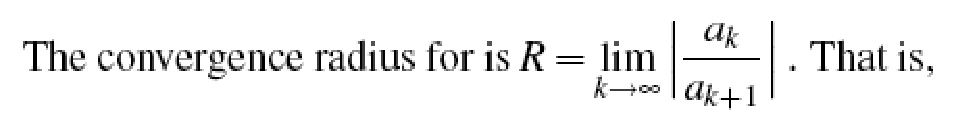
\includegraphics[width=0.55\textwidth]{latex}}}}
\subfigure{\label{word}}\addtocounter{subfigure}{-2}
\subfigure[Inline mode equation displayed as .doc format file derived from word software]{\subfigure[由~word软件生成的~.doc~格式行内公式]
          {\fbox{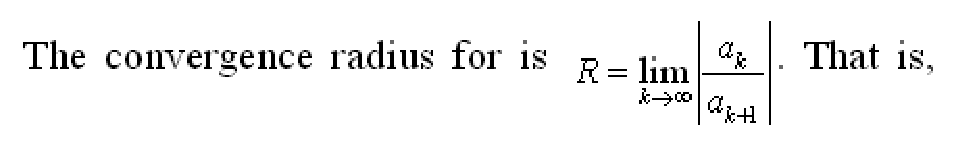
\includegraphics[width=0.55\textwidth]{word}}}}
\subfigure{\label{pdf}}\addtocounter{subfigure}{-2}
\subfigure[Inline mode equation displayed as .pdf format file derived from word software]{\subfigure[由~word软件生成的~.pdf~格式行内公式]
          {\fbox{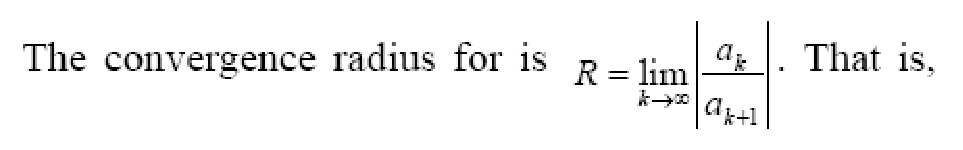
\includegraphics[width=0.55\textwidth]{pdf}}}}
\bicaption[hangju]{}{由~\LaTeX~和~word~生成的~3~种行内公式屏显效果}{Fig.$\!$}{Three kinds of inline mode equation displayed effects derived from \LaTeX and word}
\vspace{-1em}
\end{figure}
这三幅图分别为~\LaTeX~和~word~生成的行内公式屏显效果,从图中可看出,在~\LaTeX~文本含有公式的行内,在正文与公式之间对接工整,行距不变;而在~word~文本含有公式的行内,在正文与公式之间对接不齐,行距变大。因此从这一点来说,
\LaTeX~系统在数学公式的排版上具有很大优势。

\LaTeX~提供的行内公式最简单、最有效的方法是采用~\TeX~本来的标记———开始和结束标记都写作~\$,例如本节开始的例子可由下面的输入得到。
\verb|$f(x)=\int_{a}^{b}\frac{\sin{x}}{x}\mathrm{d}x$|

\BiSection{行间公式}{Displaymath mode equations}
位于两行之间的公式称为行间公式,每个公式都是一个单独的段落,例如
\[\int_a^b{f\left(x\right)\mathrm{d}x}=\lim_{\left\|\Delta{x_i}\right\|\to 0}\sum_i{f\left(\xi_i\right)\Delta{x_i}}\]
除人工编号外,\LaTeX~各种类型行间公式的标记见表~\ref{eqtag}。
\begin{table}[htbp]
\bicaption[eqtag]{}{各种类型行间公式的标记}{Table$\!$}{Tags for several kinds of displaymath mode equations}
\vspace{0.5em}\centering\wuhao
\begin{tabularx}{0.9\textwidth}{cXX}
\toprule
& 无编号 & 自动编号\\\midrule
单行公式 & \textbackslash begin\{displaymath\}...... \textbackslash end\{displaymath\}~或~\textbackslash [...\textbackslash ] & \textbackslash begin\{equation\} ...... \textbackslash end\{equation\}\\
多行公式 & \textbackslash begin\{eqnarray*\} ...... \textbackslash end\{eqnarray*\} & \textbackslash begin\{eqnarray\} ...... \textbackslash end\{eqnarray\}\\
\bottomrule
\end{tabularx}
\end{table}
另外,在自动编号的某行公式行尾添加标签~\verb|\nonumber|,可将该行转换为无编号形式。

行间多行公式需采用~\verb|eqnarray|~或~\verb|eqnarray*|~环境,它默认是一个列格式为~\verb|rcl|~的~3~列矩阵,并且中间列的字号要小一些,因此通常只将需要对齐的运算符号(通常为等号“=”)置于中间列。

\BiSection{可自动调整大小的定界符}{Delimiters with automatic adjustable sizes}
若在左右两个定界符之前分别添加命令~\verb|\left|~和~\verb|\right|,则定界符可根据所包围公式大小自动调整其尺寸,这可从式(\ref{nodelimiter})和式(\ref{delimiter})中看出。
\begin{equation}\label{nodelimiter}
(\sum_{k=\frac12}^{N^2})
\end{equation}
\begin{equation}\label{delimiter}
\left(\sum_{k=\frac12}^{N^2}\right)
\end{equation}
式(\ref{nodelimiter})和式(\ref{delimiter})是在~\LaTeX~中分别输入如下代码得到的。
\begin{lstlisting}
(\sum_{k=\frac12}^{N^2})
\left(\sum_{k=\frac12}^{N^2}\right)
\end{lstlisting}
\verb|\left|~和~\verb|\right|~总是成对出现的,若只需在公式一侧有可自动调整大小的定界符,则只要用“.”代替另一侧那个无需打印出来的定界符即可。

若想获得关于此部分内容的更多信息,可参见~\href{http://tug.ctan.org/cgi-bin/ctanPackageInformation.py?id=voss-mathmode}{Math mode}~文档的第~8~章“Brackets, braces and parentheses”。

\BiSection{数学重音符号}{Accents in math mode}
数学重音符号通常用来区分同一字母表示的不同变量,输入方法如下(需要调用~\verb|amsmath|~宏包):

\vspace{0.5em}\noindent\wuhao\begin{tabularx}{\textwidth}{Xc|Xc|Xc}
 \verb|\acute| & $\acute{a}$ & \verb|\mathring| & $\mathring{a}$ & \verb|\underbrace| & $\underbrace{a}$ \\
 \verb|\bar| & $\bar{a}$ & \verb|\overbrace| & $\overbrace{a}$ & \verb|\underleftarrow| & $\underleftarrow{a}$ \\
 \verb|\breve| & $\breve{a}$ & \verb|\overleftarrow| & $\overleftarrow{a}$ & \verb|\underleftrightarrow| & $\underleftrightarrow{a}$ \\
 \verb|\check| & $\check{a}$ & \verb|\overleftrightarrow| & $\overleftrightarrow{a}$ & \verb|\underline| & $\underline{a}$ \\
 \verb|\dddot| & $\dddot{a}$ & \verb|\overline| & $\overline{a}$ & \verb|\underrightarrow| & $\underrightarrow{a}$ \\
 \verb|\ddot| & $\ddot{a}$ & \verb|\overrightarrow| & $\overrightarrow{a}$ & \verb|\vec| & $\vec{a}$ \\
 \verb|\dot| & $\dot{a}$ & \verb|\tilde| & $\tilde{a}$ & \verb|\widehat| & $\widehat{a}$ \\
 \verb|\grave| & $\grave{a}$ & \verb|\underbar| & $\underbar{a}$ & \verb|\widetilde| & $\widetilde{a}$ \\
 \verb|\hat| & $\hat{a}$ 
\end{tabularx}\vspace{0.5em}
\xiaosi 当需要在字母~$i$~和~$j$~的上方添加重音符号时,为了去掉这两个字母顶上的小点,这两个字母应该分别改用~\verb|\imath|~和~\verb|\jmath|。

如果遇到某些符号不知道该采用什么命令能输出它时,则可通过~\href{http://detexify.kirelabs.org/classify.html}{Detexify$^2$~网站}来获取符号命令。若用鼠标左键在此网页的方框区域内画出你所要找的符号形状,则会在网页右方列出和你所画符号形状相近的~5~个符号及其相对应的~\LaTeX~输入命令。若所列出的符号中不包括你所要找的符号,还可通过点击“Select from the complete list!”的链接以得分从低到高的顺序列出所有符号及其相对应的~\LaTeX~输入命令。

最后,笔者建议大家还是要以~\href{http://tug.ctan.org/cgi-bin/ctanPackageInformation.py?id=voss-mathmode}{Math mode}~这篇~pdf~文档作为主要参考。若要获得最为标准、美观的数学公式排版形式,可以查查文档中是否有和你所要的排版形式相同或相近的代码段,通过修改代码段以获得你所要的数学公式排版形式。










% !Mode:: "TeX:UTF-8" 

\BiChapter{模板的其它说明}{Other explanation about the template}

\BiSection{中英文封面的相关信息}{Related information in Chinese and English covers}
国内图书分类号(Classif\/ied Index)的查询网址:

\centerline{\href{http://www.ztflh.com/}{http://www.ztflh.com/}——中国图书馆分类法}
国际图书分类法(U.D.C)的查询网址:

\centerline{\href{http://www.udcc.org/udcsummary/php/index.php}{http://www.udcc.org/udcsummary/php/index.php}——UDC Summary}
学校代码查询网址:

\centerline{\href{http://www.marry360.com.cn/Tools/UniversityCodeList.aspx}{http://www.marry360.com.cn/Tools/UniversityCodeList.aspx}——高校代码查询}
\noindent 哈尔滨工业大学的学校代码为~10213。

英文封面下方的学位论文相关信息可以采用~\verb|tabular|~和~\verb|tabularx|~两种表格环境,具体使用哪一种环境和具体的相关信息有关。若信息内容不太长,不会引起信息内容分行时,则应该采用~\verb|tabular|~环境;若信息内容过长,会引起信息内容分行时,则应该采用~\verb|tabularx|~环境。具体用法请见~format.tex~文件的相应代码。

\BiSection{\textsc{Bib}\kern-.08em\TeX~文献文件的写法}{How to write the \textsc{Bib}\kern-.08em\TeX~bibliographic file}
用在~\LaTeX~中的~\textsc{Bib}\kern-.08em\TeX~文献文件的扩展名为~bib,此模板中,该文件即为~reference.bib。bibtex.exe 命令根据~GBT7714-2005NLang-HIT.bst 文件定义的文献格式,将~reference.bib 中的文献数据转换为输出文档中的文献列表。GBT7714-2005NLang-HIT.bst 文件是在~\href{http://bbs.ctex.org/attachment.php?aid=MjA3MDh8ZDcyMjc2MTN8MTMyNTYzNjY4OHxhZTg4bkNCUVJiRzA0WmU3TmlMbVdTUVExa0xtV2puWWc0dkdqbVJhbTVMdy9mVQ\%3D\%3D}{GBT7714-2005NLang-UTF8.bst} 文件的基础上修改得到的,所做的唯一一处改动是将姓氏字母全部大写的英文作者名改为只首字母大写,以保证和\href{http://219.217.226.141/xuewei/guifan.doc}{《研究生学位论文撰写规范》}及其\href{http://219.217.226.141/xuewei/fanli.doc}{《研究生学位论文书写范例》}相一致。

bib 文件的编写方法可参考模板中已给出的例子,也可参考~\href{http://bbs.ctex.org/attachment.php?aid=MTk3OTd8NjY1ODc5OGV8MTMyNTY0MTEyMnxhZGZkYWpsa0I2RGZwNDR5Z1lyeStjb1dKRS8rTnJub3lvT2FkNDNJbHl1UWVkVQ\%3D\%3D}{GBT7714-2005.bst说明文档20060919
} 中所给出的例子。

中文文献需要添加一个额外的~language 域,并使得域值非空,这样~bst 文件就能够判断此文献为中文文献,进而能正确地生成参考文献格式。

GBT7714-2005.bst 对于国标~GB/T 7714-2005 的文献分类如表~\ref{tab:entrytypes} 所示。对于每种文献类型的缺省类型,已经设置好相应的文献标识码,因此不需要输入相应的文献
标识码。扩展类型的文献则应再添加一个~TypeofLit 域,并需要将其域值改为相应的文献标识码。
\begin{table}[htbp]
\bicaption[tab:entrytypes]{}{GBT7714-2005.bst 的分类方式}{Table$\!$}{Classification method of GBT7714-2005.bst}
\vspace{0.5em}\centering\wuhao
\begin{tabular}{llll}
\toprule[1.5pt]
文献类型 & 缺省类型 & 扩展类型(需要手 & 主要特征\\
 &  & 工加入文献标识码) & \\
\midrule[1pt]
article & 文章[J] & 报纸中的析出文献[N] & 年,卷(期):页码\\
 &  & 在线文章[J/OL] & \\
book & 书[M] & 论文集、会议录[C] & \\
 &  & 在线书[M/OL] & \\
 &  & 汇编[G] & \\
inbook & 书的某几页[M] &  & \\
incollection & 书中析出的文章[M]// & 汇编的析出文献[G]// & 析出文献[文献标识码]//\\
 &  & 标准的析出文献[S]// & \\
proceedings &  &  & \\
inproceedings & 论文集、会议录中的 & 在线论文集、 & 析出文献[文献标识码]//\\
/conference & 析出文献[C]// & 会议录[C/OL]// & \\
mastersthesis & 毕业论文[D] &  & 类似book类\\
phdthesis & 毕业论文[D] &  & 类似book类\\
techreport & 科技报告[R] &  & 类似book类\\
misc &  & 杂项[],例如:专利[P] & 此类一般是网上文件,\\
 &  & 网上专利[P/OL] & 按照国标规定顺序\\
 &  & 网上电子公告[EB/OL] & 编码制时不输出年份\\
 &  & 磁盘[CP/DK] & \\
\bottomrule[1.5pt]
\end{tabular}
\end{table}

《研究生学位论文撰写规范》及《研究生学位论文书写范例》中所列英文参考文献例子中的文章名的每个实词首字母都大写,因此需要将英文参考文献的~title 域手动修改为每个实词首字母大写。

英文参考文献在~author 域中的作者名需要将姓置前,名置后。

\BiSection{参考文献的引用}{Citation of references}
需要将~main.tex 文件中的语句~\verb|\nocite{*}| 屏蔽掉,这样,文中未引用的参考文献就不会出现在文后的参考文献列表中。文中参考文献的引用方法:

\begin{itemize}
\item 行文引用请使用命令~\verb|\cite{引用词}|,引用效果为“\cite{lin1992}”;
\item 上标引用请使用命令~\verb|\citeup{引用词}|,引用效果为“\citeup{lin1992}”。
\end{itemize}
其中,上标引用命令~\verb|\citeup{}| 为本模板自定义的命令,其定义为
\begin{verbatim}
\newcommand{\citeup}[1]{\textsuperscript{\cite{#1}}}
\end{verbatim}

\BiSection{单层罗列环境}{Monolayer list environment}
哈工大学位论文一般可采用两种罗列环境:一种是并列条目有同样标签的~\verb|itemize|~罗列环境,另一种是具有自动排序编号符号的~\verb|enumerate|~罗列环境。这两种罗列环境的样式参数可参考图~\ref{list}。
\begin{figure}[htbp]
\centering
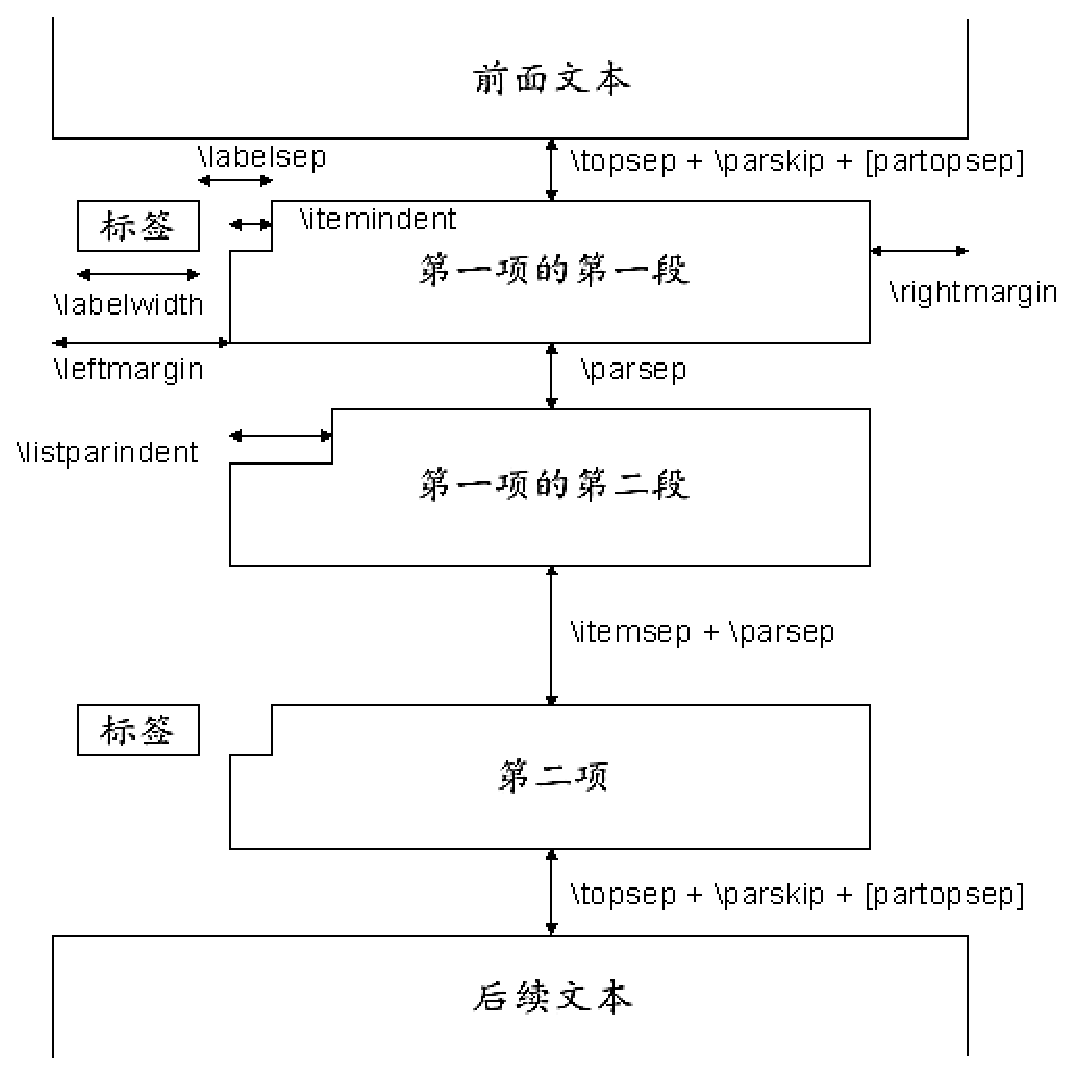
\includegraphics[width = 0.6\textwidth]{list}
\bicaption[list]{}{罗列环境参数示意图}{Fig.$\!$}{Schematic diagram of list environments}\vspace{-1em}
\end{figure}
通过调用~enumitem~宏包可以很方便地控制罗列环境的布局,其~format.tex~文件中的~\verb|\setitemize|~和~\verb|\setenumerate|~命令分别用来设置~\verb|itemize|~和~\verb|enumerate|~环境的样式参数。采用~\verb|itemize|~单层罗列环境的排版形式如下:
\begin{itemize}
\item 第一个条目文本内容
\item 第二个条目文本内容
\item 第三个条目文本内容
\end{itemize}
其代码如下
\begin{verbatim}
\begin{itemize}
  \item 第一个条目文本内容
  \item 第二个条目文本内容
  ...
  \item 第三个条目文本内容
\end{itemize}
\end{verbatim}
采用~\verb|enumerate|~单层罗列环境的排版形式如下:
\begin{enumerate}
\item 第一个条目文本内容
\item 第二个条目文本内容
\item 第三个条目文本内容
\end{enumerate}
其代码如下
\begin{verbatim}
\begin{enumerate}
  \item 第一个条目文本内容
  \item 第二个条目文本内容
  ...
  \item 第三个条目文本内容
\end{enumerate}
\end{verbatim}

\BiSection{算法}{Algorithm}

这是一个算法的例子,来自~worldguy@lilacbbs。建议将算法放在~minipage~环境中,避免算法出现在页面版心之外。

\begin{algorithm}
\KwIn{training samples, {$(d_i, d_j)_q$; $\mathbf{q}_i, \mathbf{q}_j \in C$,
$q\in \mathbf{Q}$} }
\KwOut{parameter setting $\lambda^T$}%

\For{$t$=1 to $T$}
{   
    $\lambda^{t+1}_n = \lambda^t_n + \eta (f_n(q, c, d_i) - f_n(q, c, d_j))$
 }
\end{algorithm}

%\KwIn{training samples, {$(d_i, d_j)_q$; $\mathbf{q}_i, \mathbf{q}_j \in C$,
%$q\in \mathbf{Q}$} }
%\KwOut{parameter setting $\lambda^T$}%
%
%\For{$t$=1 to $T$}
%{   
%    $\lambda^{t+1}_n = \lambda^t_n + \eta (f_n(q, c, d_i) - f_n(q, c, d_j))$
% }
%\end{algorithm}

算法环境中右侧空白比较多,若想把右侧的空白框减小,可以采用~minipage~环境实现。把~algorithm~环境放到~minipage~环境里面,并且加上选项[H]禁止算法浮动,下面给出一个例子。需要说明的是,一般不需要进行这种处理。算法标题可有可无,若有中英文标题,请使用~\verb|\AlgoBiCaption{中文标题}{英文标题}|。下面给出两个有标题的例子。需要说明的是,算法的标题是自动换行,没有必要手动换行。

\begin{minipage}{0.8\textwidth}\centering
\begin{algorithm}[H]
 \AlgoBiCaption{这是一个简短的算法中文图题}{This is the English caption of the algorithm}
  \KwIn{training samples, {$(d_i, d_j)_q$; $\mathbf{q}_i, \mathbf{q}_j
      \in C$, $q\in \mathbf{Q}$} }
 \KwOut{parameter setting
    $\lambda^T$}
 \For{$t$=1 to $T$} { $\lambda^{t+1}_n = \lambda^t_n +
    \eta (f_n(q, c, d_i) - f_n(q, c, d_j))$ }
\end{algorithm}
\end{minipage}


\begin{minipage}{0.9\textwidth}\centering
\begin{algorithm}[H]
 \AlgoBiCaption{这是一个算法的比较长的中文图题,需要换行,这里采用自动换行,如果手动换行会造成算法目录中同样出现断行}{This is a long English caption of the algorithm, a new line  required, and this a new line}
  \KwIn{training samples, {$(d_i, d_j)_q$; $\mathbf{q}_i, \mathbf{q}_j
      \in C$, $q\in \mathbf{Q}$} }
 \KwOut{parameter setting
    $\lambda^T$}
 \For{$t$=1 to $T$} { $\lambda^{t+1}_n = \lambda^t_n +
    \eta (f_n(q, c, d_i) - f_n(q, c, d_j))$ }
\end{algorithm}
\end{minipage}

\BiSection{定理定义}{Theorem and definition}

若需要书写定理定义等内容,而且带有顺序编号,需要采用如下环境。除了~\verb|proof|~环境之外,其余~9~个环境都可以有一个可选参数作为附加标题。

\begin{center}\vspace{0.5em}\noindent\wuhao\begin{tabularx}{0.7\textwidth}{lX|lX}
定理 & \verb|theorem|~环境 & 定义 & \verb|definition|~环境 \\
例 & \verb|example|~环境 & 算法 & \verb|algo|~环境 \\
公理 & \verb|axiom|~环境 & 命题 & \verb|proposition|~环境 \\
引理 & \verb|lemma|~环境 & 推论 & \verb|corollary|~环境 \\
注解 & \verb|remark|~环境 & 证明 & \verb|proof|~环境 \\
\end{tabularx}\end{center}
% !Mode:: "TeX:UTF-8" 

\BiAppendixChapter{结\quad 论}{Conclusions}

文本立场分析是挖掘文本作者对主题目标所持有的立场的技术。本课题在分析了文本立场分析在国内外的研究现状后,发现现有研究还存在以下问题:(1)现有对文本立场分析的研究途径主要集中在基于传统语义特征的机器学习,构建模型成本较高。(2)现有的文本立场分析方法通常没有考虑主题目标信息,而将文本立场分析看成简单的文本分类任务。为解决上述问题,本课题的主要工作包括以下两点:

(1)针对已有立场分析研究未引入主题目标信息的缺点,将条件编码模型引入到文本立场分析任务。使主题目标信息以一种“先验知识”的方式参与对文本的编码。根据社交立场文本的特点,本文提出分别用单向LSTM与双向LSTM编码主题目标信息与文本信息。实验结果表明以改进后条件编码的方式引入主题目标信息能显著提高文本立场分析的性能。改进后模型在SemEval2016英文立场分析数据集和NLPCC2016中文立场分析数据集的微平均F1值分别为0.671与0.698,在不需要外部收集语料与手工设计特征的前提下,所提出的方法具有较好的性能。

(2)基于主题目标对文本信息内容有着不同的侧重点为基础,本文将主题目标信息作为注意力机制的导向,给予文本信息不同权重的关注度,在不同权重文本信息中挖掘有关立场分析的模式。由于条件编码与注意力机制分别从“编码”与“解码”两个不同角度引入主题目标信息,本文提出一种融合注意力机制与条件编码的文本立场分析方法。实验表明条件编码与注意力机制方式在不同主题目标任务下各有优劣,融合后的模型具有显著的提升。融合后模型在SemEval2016英文立场分析数据集和NLPCC2016中文立场分析数据集的微平均F1值分别为0.689与0.716。对比两个数据集评测任务的最优系统均有提升,表明本文提出融合注意力机制与条件编码模型在社交媒体文本立场分析任务上的有效性。

本研究针对现有问题提出一些解决的方案,但是由于时间限制,还存在若干缺点和不足。例如,未将深度学习和传统特征机器学习方法结合,形成一个更加强健的解决方案;此外,无监督或弱监督的立场分析方法也是将来值得尝试的方向。   % 结论

%\BiChapter{图片的插入方法}{Methods of inserting figures}

\BiSection{单张图片的插入方法}{The method of inserting one single figure}

\BiSubsection{条标题}{The caption of subsection}

单张图片独自占一行的插入形式如图~\ref{golfer1}~所示。
\begin{figure}[htbp]
\centering
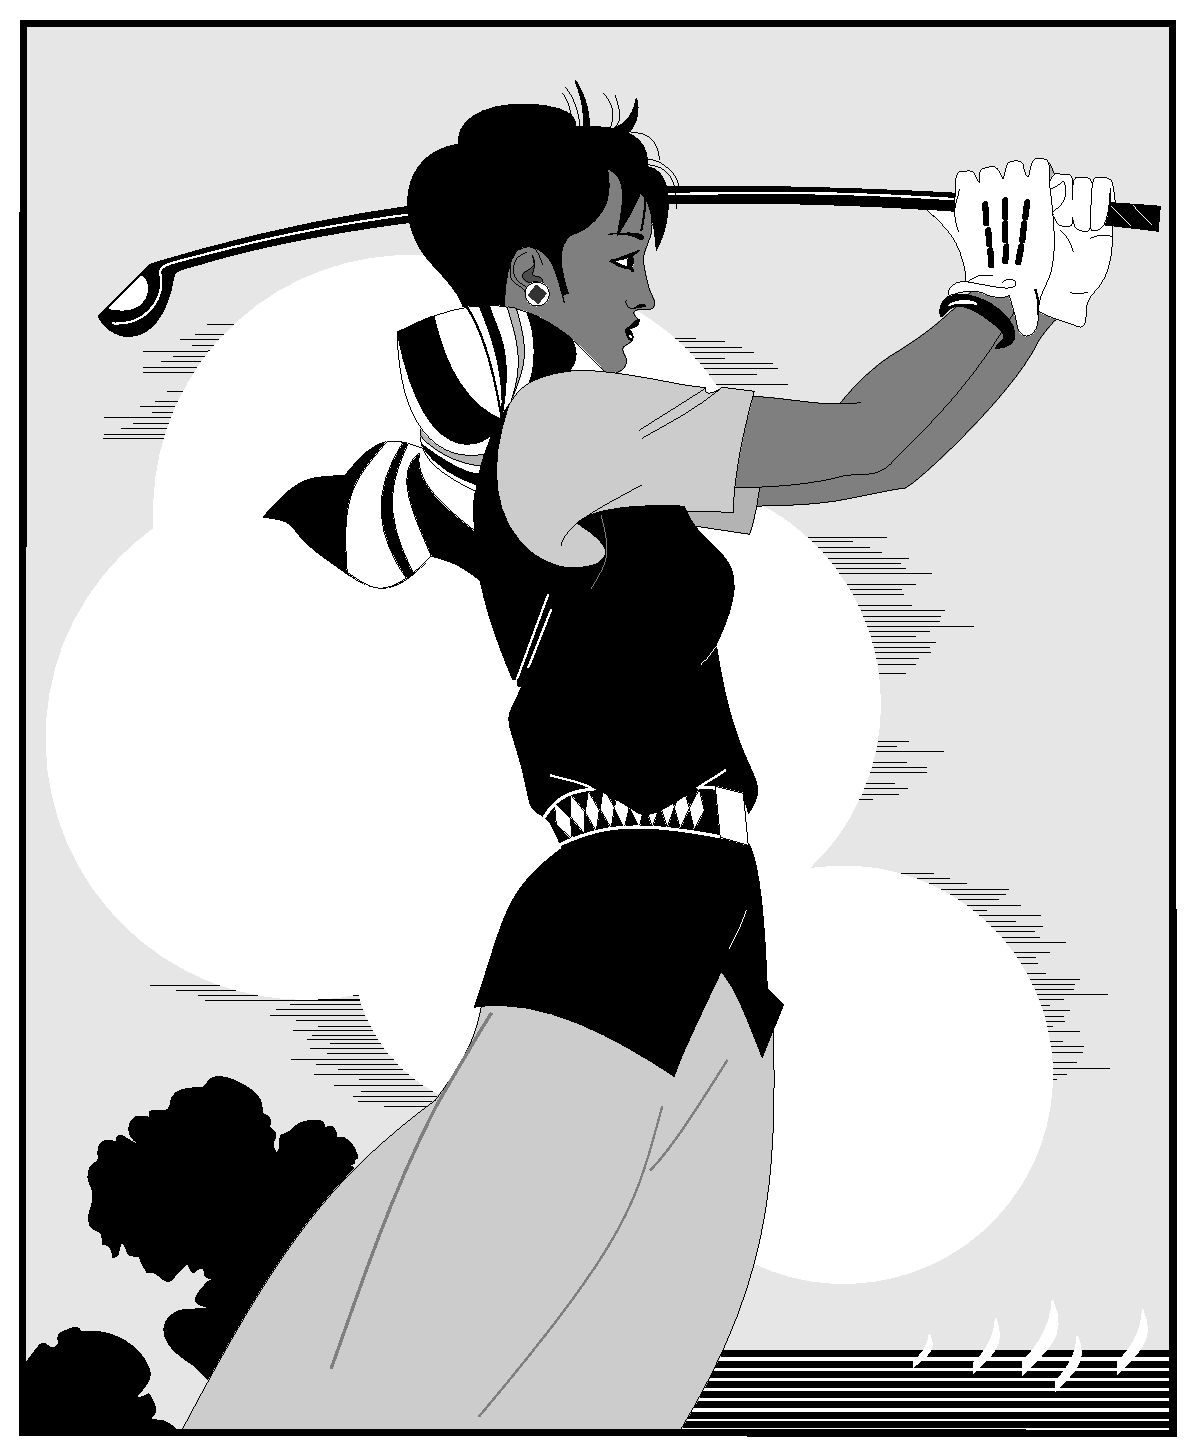
\includegraphics[width = 0.4\textwidth]{golfer}
\bicaption[golfer1]{}{打高尔夫球的人}{Fig.$\!$}{The person playing golf}\vspace{-1em}
\end{figure}

其插入图片的代码及其说明如下。
\begin{verbatim}
\begin{figure}[htbp]
\centering
\includegraphics[width=0.4\textwidth]{文件名(.eps)}
\bicaption[标签名(英文)]{}{中文标题}{Fig.$\!$}
          {English caption (首字母大写)}\vspace{-1em}
\end{figure}
\end{verbatim}
%\BiChapter{表格的绘制方法}{Methods of drawing tables}

\BiSection{普通表格的绘制方法}{Methods of drawing normal tables}


表格应具有三线表格式,因此需要调用~booktabs~宏包,其标准格式如表~\ref{table1}~所示。
\begin{table}[htbp]
\bicaption[table1]{}{符合研究生院绘图规范的表格}{Table$\!$}{Table in agreement of the standard from graduate school}
\vspace{0.5em}\centering\wuhao
\begin{tabular}{ccccc}
\toprule[1.5pt]
$D$(in) & $P_u$(lbs) & $u_u$(in) & $\beta$ & $G_f$(psi.in)\\
\midrule[1pt]
 5 & 269.8 & 0.000674 & 1.79 & 0.04089\\
10 & 421.0 & 0.001035 & 3.59 & 0.04089\\
20 & 640.2 & 0.001565 & 7.18 & 0.04089\\
\bottomrule[1.5pt]
\end{tabular}
\end{table}

其绘制表格的代码及其说明如下。
\begin{verbatim}
\begin{table}[htbp]
\bicaption[标签名]{}{中文标题}{Table$\!$}{English caption}
\vspace{0.5em}\centering\wuhao
\begin{tabular}{cc...c}
\toprule[1.5pt]
表头第1个格   & 表头第2个格   & ... & 表头第n个格  \\
\midrule[1pt]
表中数据(1,1) & 表中数据(1,2) & ... & 表中数据(1,n)\\
表中数据(2,1) & 表中数据(2,2) & ... & 表中数据(2,n)\\
...................................................\\
表中数据(m,1) & 表中数据(m,2) & ... & 表中数据(m,n)\\
\bottomrule[1.5pt]
\end{tabular}
\end{table}
\end{verbatim}
%\BiChapter{数学公式的输入方法}{Input methods of equations}

\BiSection{行内公式}{Inline mode equations}

出现在正文一行之内的公式称为行内公式,例如~$f(x)=\int_{a}^{b}\frac{\sin{x}}{x}\mathrm{d}x$。对于非矩阵和非多行形式的行内公式,一般不会使得行距发生变化。

\BiSection{行间公式}{Displaymath mode equations}

位于两行之间的公式称为行间公式,每个公式都是一个单独的段落,下边的例子是一个无编号的行间单行公式

\[
\int_a^b{f\left(x\right)\mathrm{d}x}=\lim_{\left\|\Delta{x_i}\right\|\to 0}\sum_i{f\left(\xi_i\right)\Delta{x_i}}
\]

下边的例子是一个无编号的行间多行公式(\ref{lizi})
\begin{eqnarray*}\label{lizi}
\sin 2x&=&2\sin x\cos x\\
\cos 2x&=&2\cos x^2-1=1-2\sin x^2=\cos x^2-\sin x^2
\end{eqnarray*}
%参考文献\cite{OOSTRUM01}和参考文献\citeup{wwwlixing}


%参考文献
\defaultfont
\bibliographystyle{GBT7714-2005NLang-HIT}
\addcontentsline{toc}{chapter}{参考文献}      % 参考文献加入到中文目录
\addcontentsline{toe}{chapter}{\bfseries  References} % 参考文献加入到英文目录
\addtolength{\bibsep}{-0.8em}
%\nocite{*}  %若将此命令屏蔽掉,则未引用的文献不会出现在文后的参考文献列表中。
\bibliography{reference}
\renewcommand{\appendixname}{附录~\Alph{chapter}}
\renewcommand{\theequation}{\Alph{chapter}-\arabic{equation}}
\renewcommand{\thetable}{\Alph{chapter}-\arabic{table}}
% -*-coding: utf-8 -*-

\defaultfont
\appendix

%%%%%%%%%%%%%%%%%%%%%%%%%%%%%%%%%%%%%%%%%%%%%%%%%%%%%%%%%
\BiAppChapter{带章节的附录}{Full Appendix}
完整的附录内容,包含章节,公式,图表等

%%%%%%%%%%%%%%%%%%%%%%%%%%%%%%%%%%%%%%%%%%%%%%%%%%%%%%%%%
\BiSection{附录节的内容}{Section in Appendix}
这是附录的节的内容

附录中图的示例:
\begin{figure}[htbp]
\centering
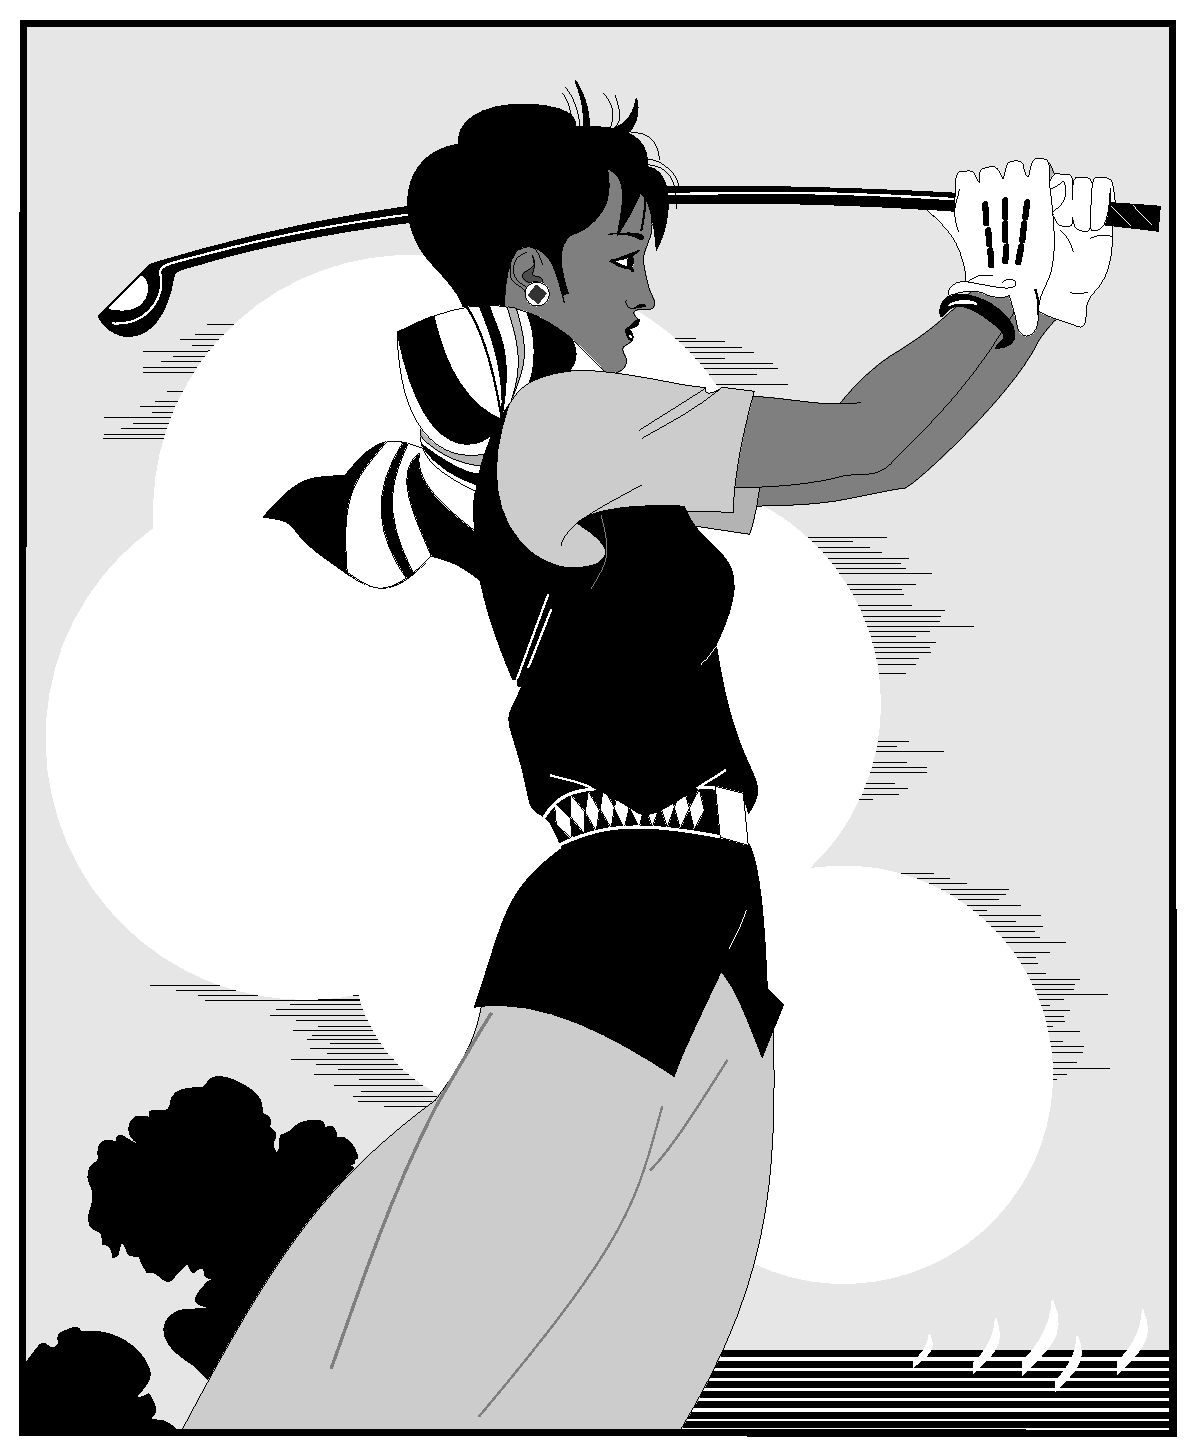
\includegraphics[width = 0.4\textwidth]{golfer}
\bicaption[golfer5]{}{打高尔夫球的人}{Fig.$\!$}{The person playing golf}\vspace{-1em}
\end{figure}

附录中公式的示例:
\begin{align}
a & = b \times c \\
E & = m c^2
\end{align}

\BiAppChapter{这个星球上最好的免费Windows软件列表}{List of the Best Free Windows Software in our Planet}
\section*{杀毒软件}
\href{http://www.avast.com/zh-cn/free-antivirus-download}{avast! 免费杀毒软件}——推荐

\href{http://www.avg.com/cn-zh/china-avg-antivirus-free}{AVG 杀毒永久免费版}——推荐

\href{http://www.avira.com/en/avira-free-antivirus}{Avira Free Antivirus (小红伞)}









%\BiAppChapter{附录三}{appendix 3}    % 附录
% !Mode:: "TeX:UTF-8" 

\BiAppendixChapter{攻读\cxuewei 学位期间发表的论文及其他成果} {Papers
published in the period of PH.D. education}
\noindent\textbf{(一)发表的学术论文}
\begin{publist}
\item	\underline{XXX},XXX. Static Oxidation Model of Al-Mg/C Dissipation Thermal Protection Materials[J]. Rare Metal Materials and Engineering, 2010, 39(Suppl. 1): 520-524.(SCI~收录,IDS号为~669JS,IF=0.16)
\item XXX,\underline{XXX}. 精密超声振动切削单晶铜的计算机仿真研究[J]. 系统仿真学报,2007,19(4):738-741,753.(EI~收录号:20071310514841)
\item XXX,XXX. 局部多孔质气体静压轴向轴承静态特性的数值求解[J]. 摩擦学学报,2007(1):68-72.(EI~收录号:20071510544816)
\item XXX,XXX. 硬脆光学晶体材料超精密切削理论研究综述[J]. 机械工程学报,2003,39(8):15-22.(EI~收录号:2004088028875)
\item XXX,XXX. 基于遗传算法的超精密切削加工表面粗糙度预测模型的参数辨识以及切削参数优化[J]. 机械工程学报,2005,41(11):158-162.(EI~收录号:2006039650087)
\item XXX,XXX. Discrete Sliding Mode Cintrok with Fuzzy Adaptive Reaching Law on 6-PEES Parallel Robot[C]. Intelligent System Design and Applications, Jinan, 2006: 649-652.(EI~收录号:20073210746529)
\end{publist}

\noindent\textbf{(二)申请及已获得的专利(无专利时此项不必列出)}
\begin{publist}
\item XXX,XXX. 一种温热外敷药制备方案:中国,88105607.3[P]. 1989-07-26.
\end{publist}

\noindent\textbf{(三)参与的科研项目及获奖情况}
\begin{publist}
\item	XXX,XXX. XX~气体静压轴承技术研究, XX~省自然科学基金项目.课题编号:XXXX.
\item XXX,XXX. XX~静载下预应力混凝土房屋结构设计统一理论. 黑江省科学技术二等奖, 2007.
\end{publist}
%\vfill
%\hangafter=1\hangindent=2em\noindent

%\setlength{\parindent}{2em}
    % 所发文章
% !Mode:: "TeX:UTF-8" 

\BiAppendixChapter{哈尔滨工业大学学位论文原创性声明和使用权限}{Statement of copyright and Letter of authorization}
\vspace{\baselineskip}
\begin{center}\hei\xiaosan{学位论文原创性声明}\end{center}
\vspace{1em}

本人郑重声明:此处所提交的学位论文《\chinesethesistitle》,是本人在导师指导下,在哈尔滨工业大学攻读学位期间独立进行研究工作所取得的成果,且学位论文中除已标注引用文献的部分外不包含他人完成或已发表的研究成果。对本学位论文的研究工作做出重要贡献的个人和集体,均已在文中以明确方式注明。

\vspace{\baselineskip}
\hspace{6em}作者签名:\hfill 日期:\hspace{2.5em}年\hspace{1.5em}月\hspace{1.5em}日

\vspace{2\baselineskip}
\begin{center}\hei\xiaosan{学位论文使用权限}\end{center}
\vspace{1em}

学位论文是研究生在哈尔滨工业大学攻读学位期间完成的成果,知识产权归属哈尔滨工业大学。学位论文的使用权限如下:

(1)学校可以采用影印、缩印或其他复制手段保存研究生上交的学位论文,并向国家图书馆报送学位论文;(2)学校可以将学位论文部分或全部内容编入有关数据库进行检索和提供相应阅览服务;(3)研究生毕业后发表与此学位论文研究成果相关的学术论文和其他成果时,应征得导师同意,且第一署名单位为哈尔滨工业大学。

保密论文在保密期内遵守有关保密规定,解密后适用于此使用权限规定。

本人知悉学位论文的使用权限,并将遵守有关规定。


\vspace{2\baselineskip}
\hspace{6em}作者签名:\hfill 日期:\hspace{2.5em}年\hspace{1.5em}月\hspace{1.5em}日

\vspace{2\baselineskip}
\hspace{6em}导师签名:\hfill 日期:\hspace{2.5em}年\hspace{1.5em}月\hspace{1.5em}日   % 承诺
% !Mode:: "TeX:UTF-8" 

\BiAppendixChapter{致\quad 谢}{Acknowledgements}

衷心感谢导师徐睿峰教授对本人的精心指导。在徐老师的悉心指导下完成了本论文。

在研究生期间,徐老师以其渊博的专业知识和严谨的治学态度指导我们进行学术研究,使我收益非浅。在论文的撰写期间,徐老师投入了大量的时间和精力帮助论文的修改,提高了论文的质量。在生活上,徐老师也经常给予关心,组织了各种集体活动,丰富我们的课余生活。

感谢研究中心的王晓龙老师、陈清财老师、丁宇新老师、刘滨老师、汤步洲老师和徐军老师对我的指导和点拨,他们在科研和教书育人中的严谨态度和执着精神让我受益良多。

感谢陈涛、桂林、周继云,杜嘉晨师兄,在学习和科研中得到了师兄们的很多帮助,也在师兄身上学到了很多做事的道理,尤其杜嘉晨师兄,在课题的研究方向上给予了很多宝贵的建议和指导。

感谢实验同级的夏晓玲、赵志山、胡健楠、温志渊、陈晟和郑志辉三年来大家奋战在一起,希望每个人都有美好的前程。

感谢我的父母和姐姐,感谢他们的关爱与照顾。

本课题承蒙自然科学基金基金资助、广东省自然科学基金和深圳市基础研究计划的资助,特此致谢。
% 致谢

\ifxueweidoctor
% !Mode:: "TeX:UTF-8" 

\defaultfont

\BiAppendixChapter{个人简历}{Resume}

XXXX~年~XX~月~XX~日出生于~XXXX。

XXXX~年~XX~月考入~XX~大学~XX~院(系)XX~专业,XXXX~年~XX~月本科毕业并获得~XX~学学士学位。

XXXX~年~XX~月------XXXX~年~XX~月在~XX~大学~XX~院(系)XX~学科学习并获得~XX~学硕士学位。

XXXX~年~XX~月------XXXX~年~XX~月在~XX~大学~XX~院(系)XX~学科学习并获得~XX~学博士学位。

获奖情况:如获三好学生、优秀团干部、X~奖学金等(不含科研学术获奖)。

工作经历:

\vspace{3em}\noindent
\textbf{( 除全日制硕士生以外,其余学生均应增列此项。个人简历一般应包含教育经历和工作经历。)}          % 博士学位论文有个人简介
\fi

\clearpage

\end{document} 
